%%===========================================================%%
%%                                                           %%
%%                    PHYSICS RESULTS                        %%
%%                                                           %%
%%===========================================================%%


\chapter{Physics results}\label{chap:physicsResults}

\section{Differential cross sections}

In this subsection we present differential fiducial cross sections.

\begin{figure}[h]
\centering
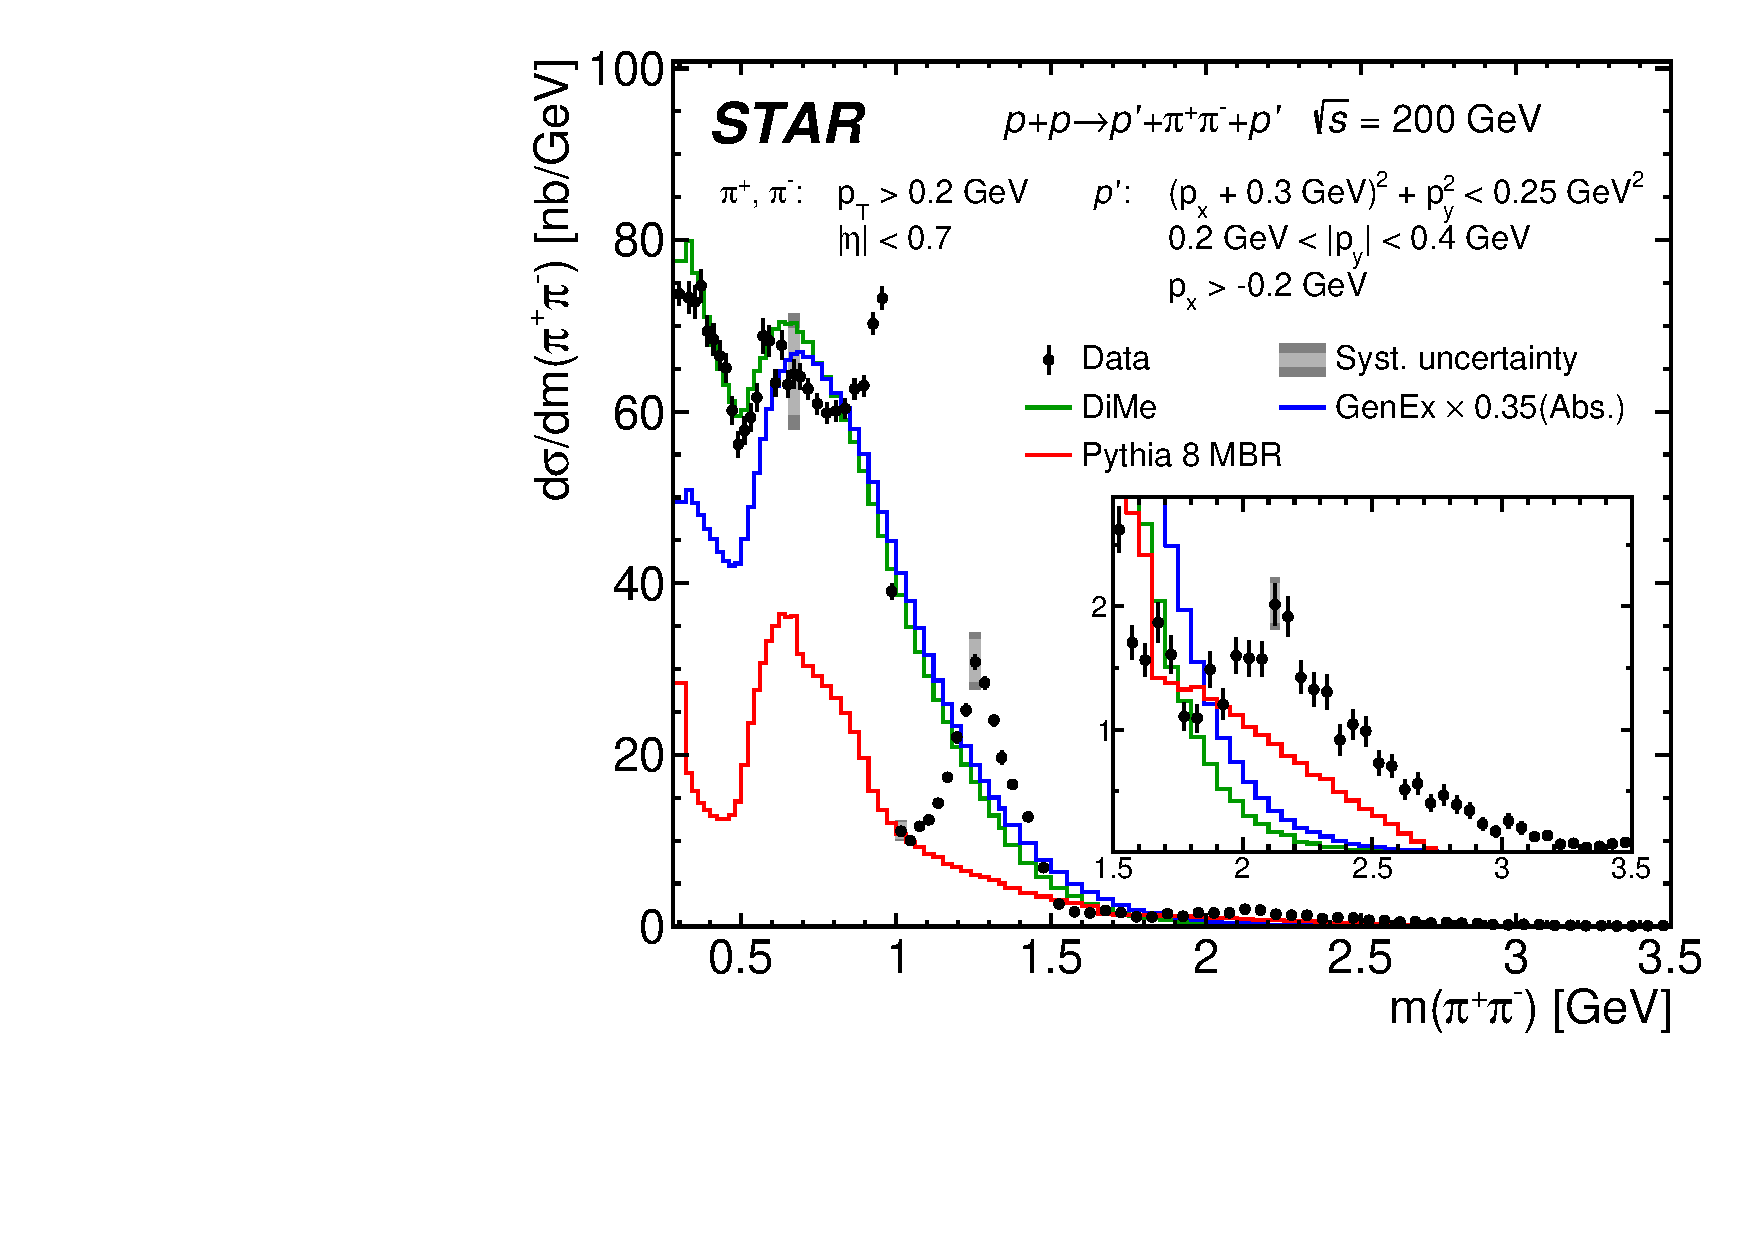
\includegraphics[width=.7\textwidth,page=1]{graphics/physicsResults/FinalResult_InvMass_pion.pdf}
%
\caption[Differential cross sections for CEP of charged particle pairs $\pi^+\pi^-$ as a function of the invariant mass of the pair in the fiducial region.]{Differential cross sections for CEP of charged particle pairs $\pi^+\pi^-$ as a function of the invariant mass of the pair in the fiducial region explained on the plots. Data are shown as solid points with error bars representing the statistical uncertainties. The typical systematic uncertainties are shown as gray boxes for only few data points as they are almost fully correlated between neighboring bins. Predictions from MC models GenEx, DiMe and MBR are shown as histograms. In the lower panels in the bottom plots the ratios of the MC predictions scaled to data and the data are shown.}
\label{results_01}
\end{figure}
%
\begin{figure}[h]
\centering
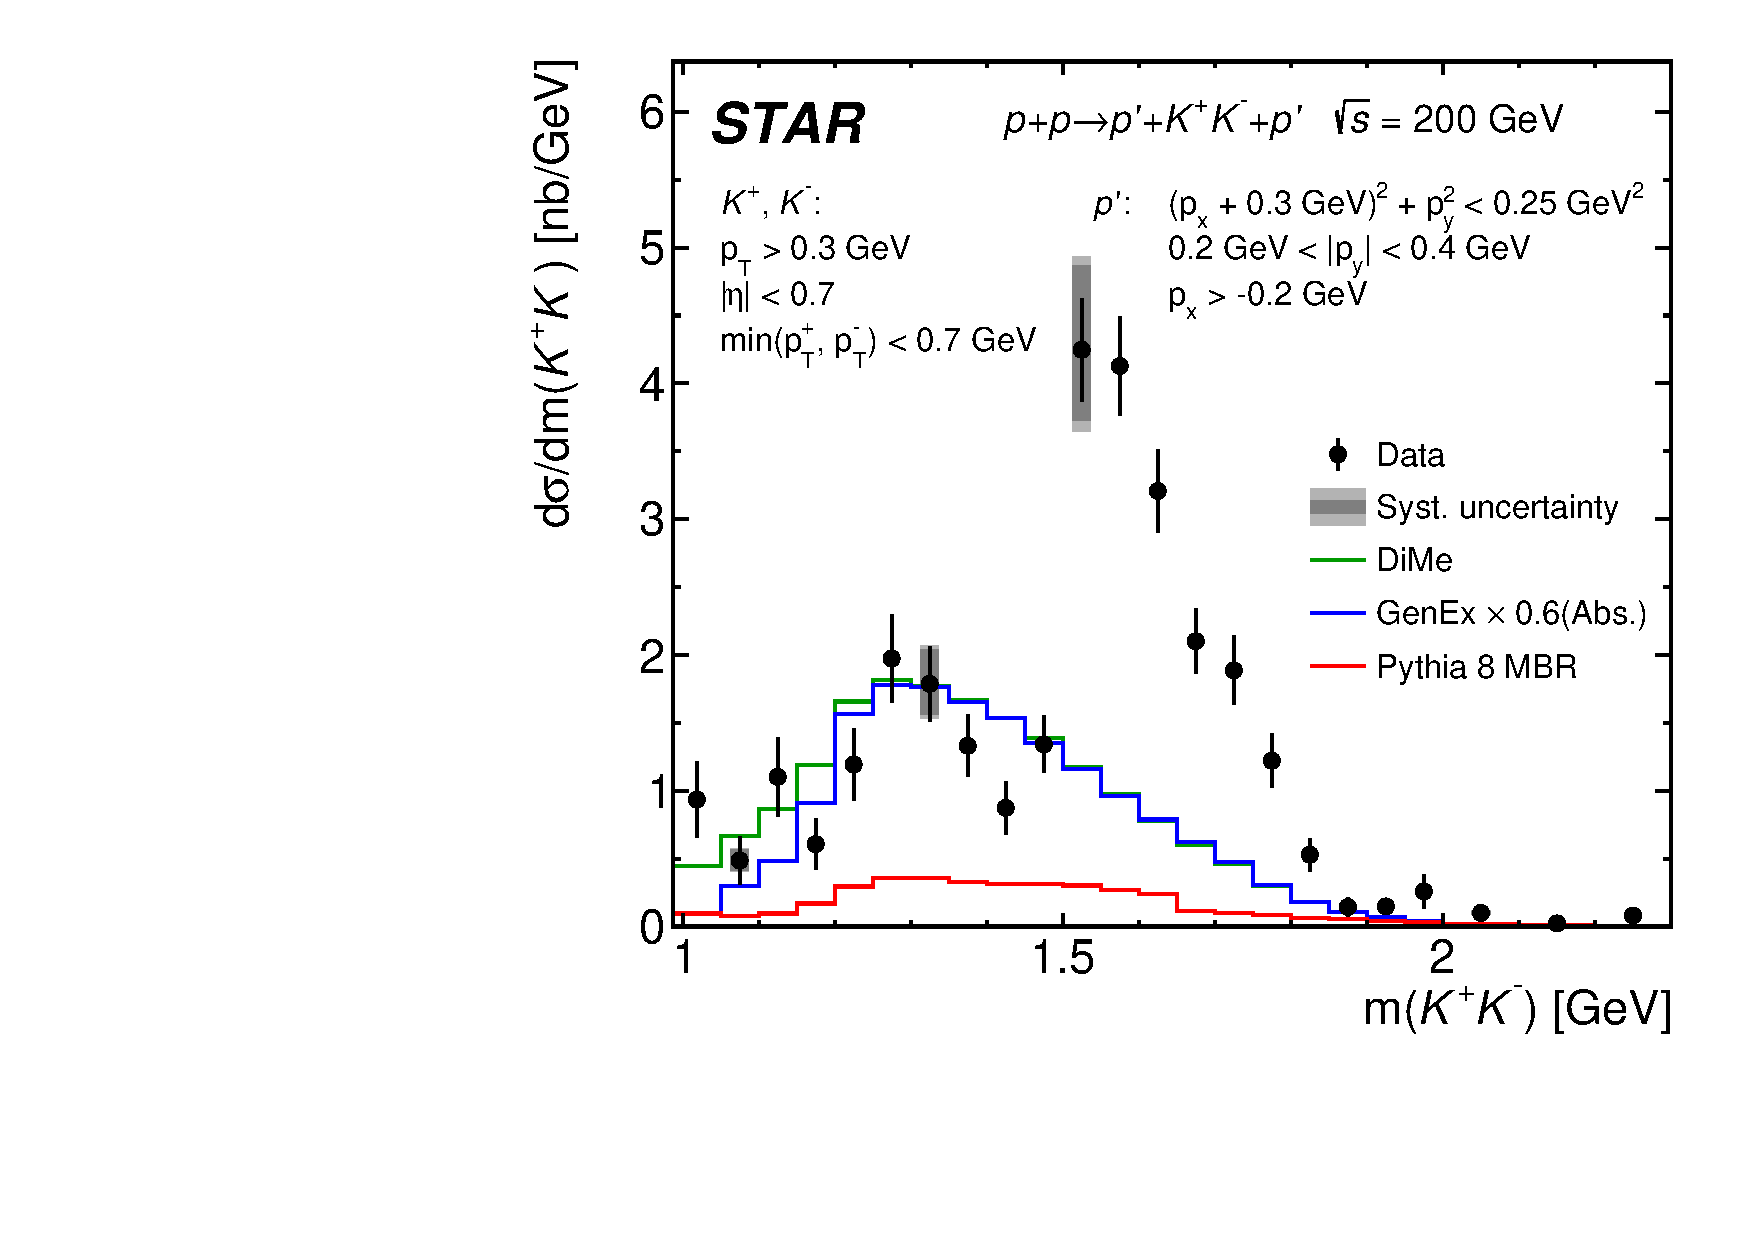
\includegraphics[width=.48\textwidth,page=1]{graphics/physicsResults/FinalResult_InvMass_kaon.pdf}
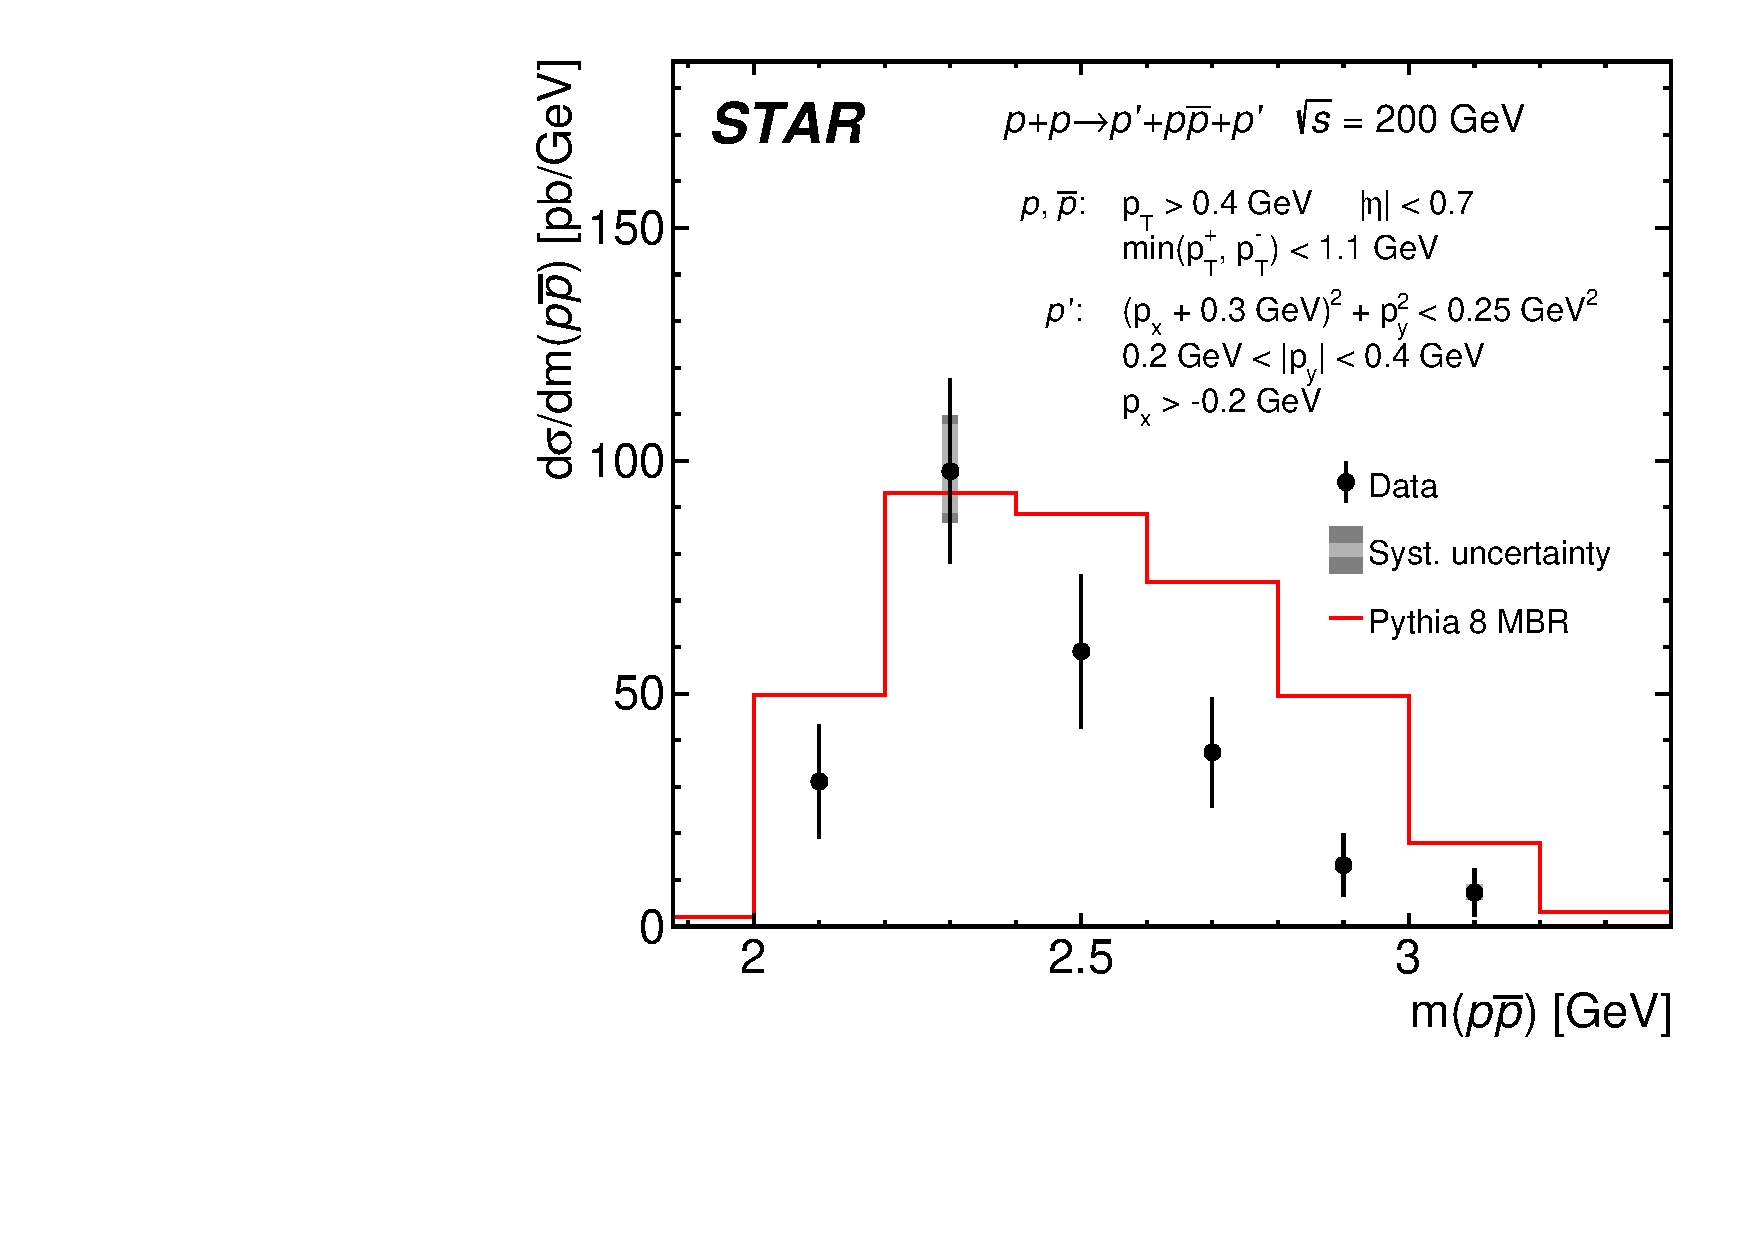
\includegraphics[width=.48\textwidth,page=1]{graphics/physicsResults/FinalResult_InvMass_proton.pdf}
%
\caption[Differential cross sections for CEP of charged particle pairs $K^+K^-$ and $p\bar{p}$ as a function of the invariant mass of the pair in the fiducial region.]{Differential cross sections for CEP of charged particle pairs $K^+K^-$ (left) and $p\bar{p}$ (right) as a function of the invariant mass of the pair in the fiducial region explained on the plots. Data are shown as solid points with error bars representing the statistical uncertainties. The typical systematic uncertainties are shown as gray boxes for only few data points as they are almost fully correlated between neighboring bins. Predictions from MC models GenEx, DiMe and MBR are shown as histograms. In the lower panels in the bottom plots the ratios of the MC predictions scaled to data and the data are shown.}
\label{results_02}
\end{figure}
% 
\begin{figure}[h]
\centering
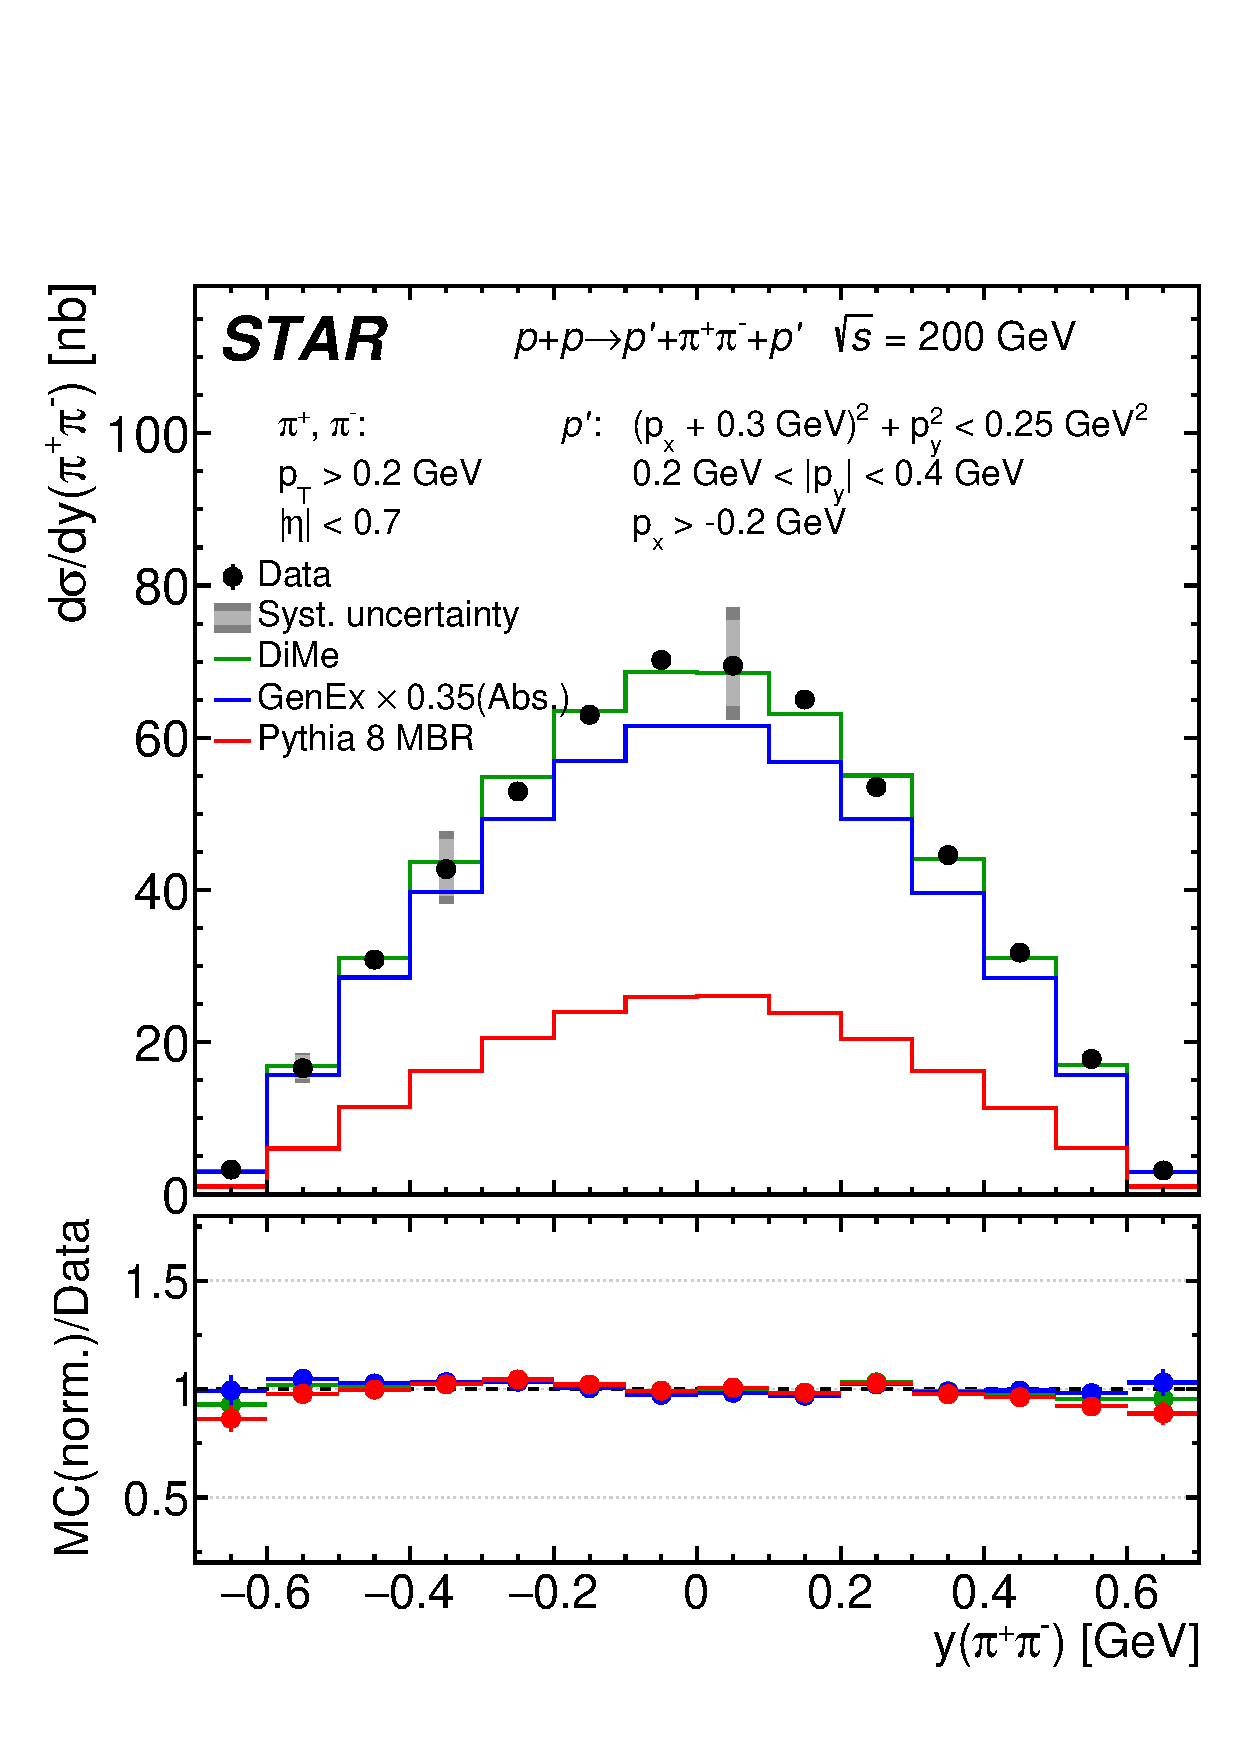
\includegraphics[width=.31\textwidth,page=1]{graphics/physicsResults/Ratio_FinalResult_Rapidity_pion.pdf}
\hfill
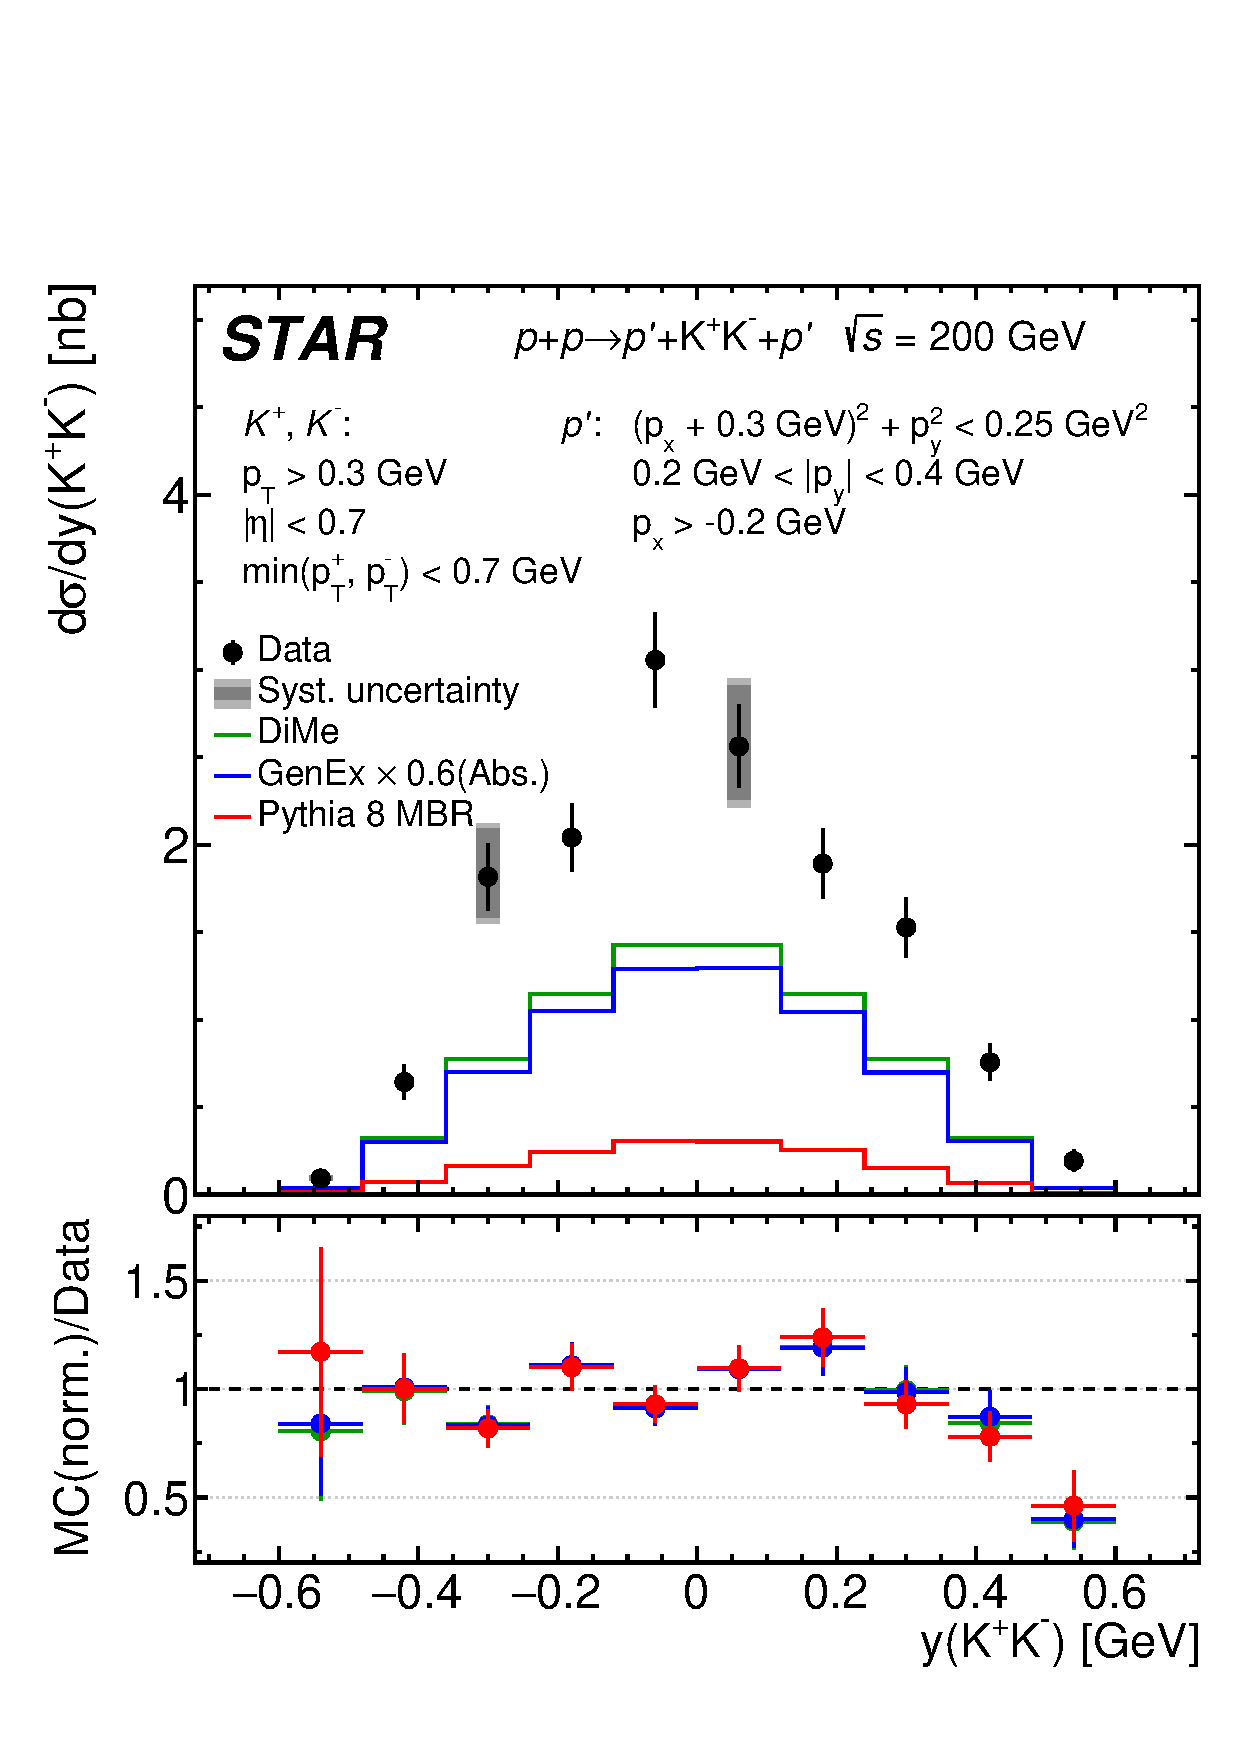
\includegraphics[width=.31\textwidth,page=1]{graphics/physicsResults/Ratio_FinalResult_Rapidity_kaon.pdf}
\hfill
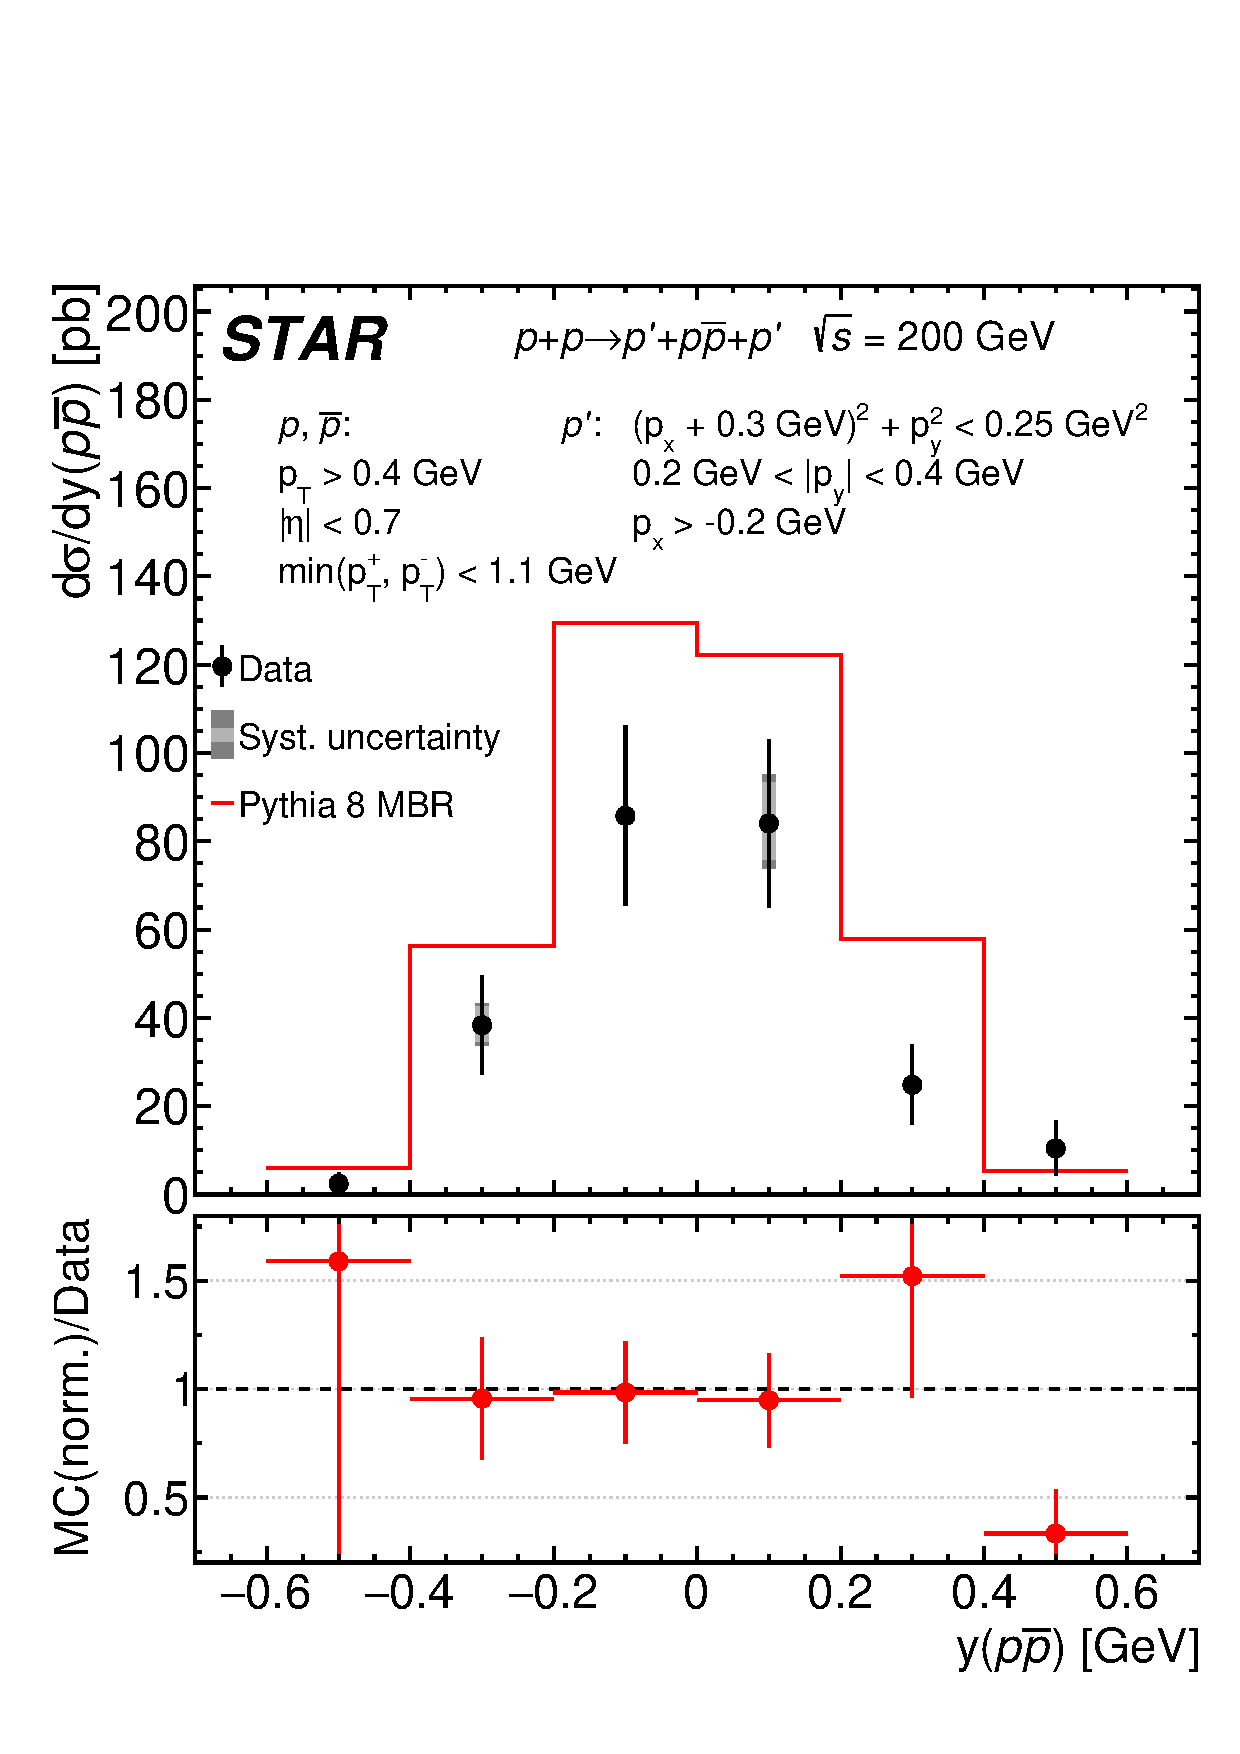
\includegraphics[width=.31\textwidth,page=1]{graphics/physicsResults/Ratio_FinalResult_Rapidity_proton.pdf}
%
\caption[Differential cross sections for CEP of charged particle pairs $\pi^+\pi^-$, $K^+K^-$ and $p\bar{p}$ as a function of the pair rapidity measured in the fiducial region.]{Differential cross sections for CEP of charged particle pairs $\pi^+\pi^-$ (left), $K^+K^-$ (middle) and $p\bar{p}$ (right) as a function of the pair rapidity measured in the fiducial region explained on the plots. Data are shown as solid points with error bars representing the statistical uncertainties. The typical systematic uncertainties are shown as gray boxes for only few data points as they are almost fully correlated between neighboring bins. Predictions from MC models GenEx, DiMe and MBR are shown as histograms. In the lower panels in the bottom plots the ratios of the MC predictions scaled to data and the data are shown.}
\label{results_1}
\end{figure}
%
% \indent
% Figure~\ref{results_2}(right column) shows the differential cross sections for CEP of different particle species pairs as a function of the sum of the squares of the four-momenta transfers at the proton vertices.
% %
% The shapes of measured cross sections are strongly affected by the fiducial cuts applied to the forward scattered protons.
% %
% The shapes of the differential cross sections for both $\pi^+\pi^-$ snd $K^+K^-$ pairs production are better described by the DiMe model than by GenEx and MBR models.
% In case of the cross section for $p\bar{p}$ pairs production the MBR model implemented in PYTHIA8 describes normalization of the data fairly well but predicts a steeper slope.\\
% %
% \indent
% Figure~\ref{results_3} shows the differential cross sections for CEP of different particle species pairs as a function of the pair invariant mass separately in two $\Delta\phi$ regions: $\Delta\phi<90$ degree (left column) and $\Delta\phi>90$ degree (right column).
% %
% Sharp drops of the measured cross sections at $m(\pi^+\pi^-) < 0.6$~GeV and at $m(K^+K^-) < 1.3$~GeV for the $\Delta\phi>$ 90 degree range are due to the fiducial cuts applied to the forward scattered protons. 
% %
% In case of the cross section for CEP of $\pi^+\pi^-$ pairs in $\Delta\phi<90$ degree range the peak around $f_2(1270)$ resonance in data is significantly suppressed while the peak at $f_0(980)$ is enhanced as well as possible resonances in the mass range $1.3-1.5$ MeV compared to the $\Delta\phi>90$ degrees range. 
%
\begin{figure}[h]
\centering
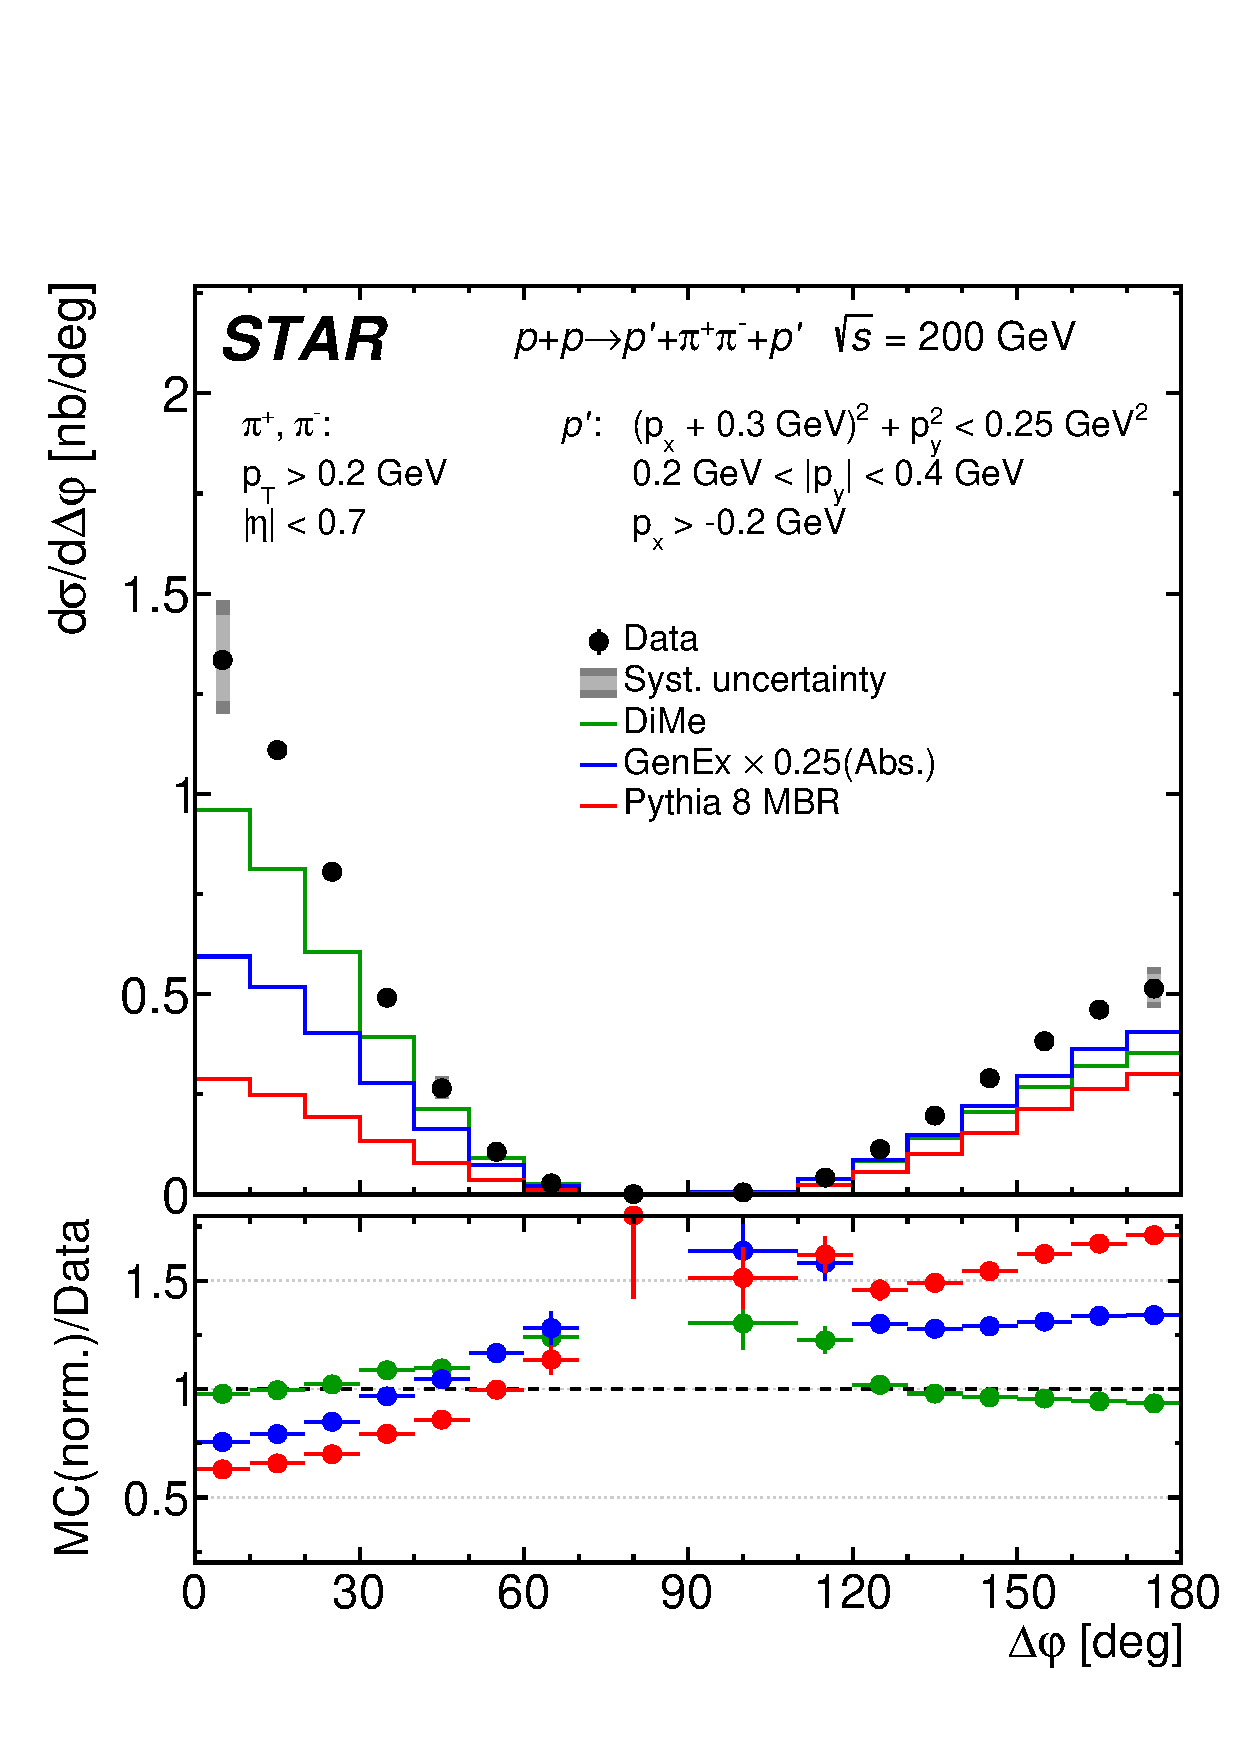
\includegraphics[width=.31\textwidth,page=1]{graphics/physicsResults/Ratio_FinalResult_DeltaPhi_pion.pdf}
\hfill
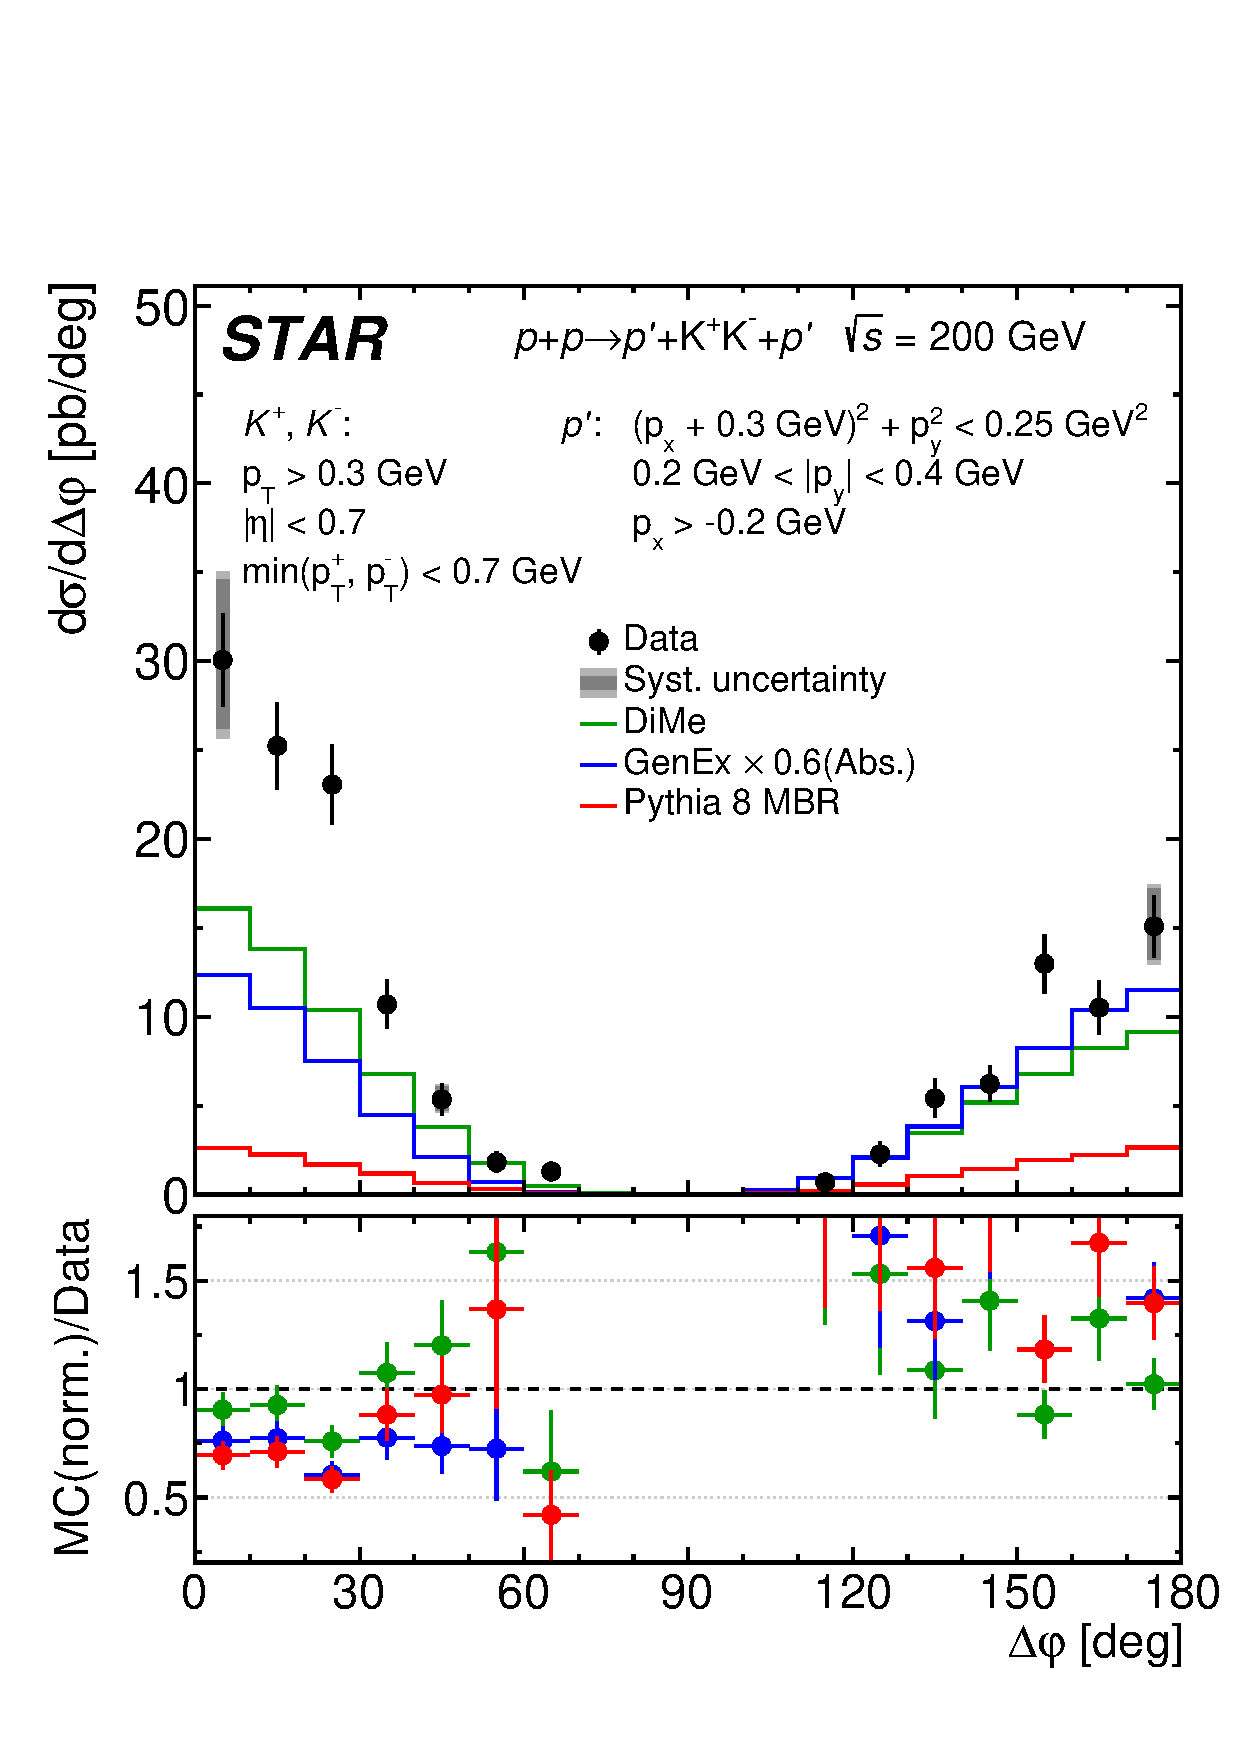
\includegraphics[width=.31\textwidth,page=1]{graphics/physicsResults/Ratio_FinalResult_DeltaPhi_kaon.pdf}
\hfill
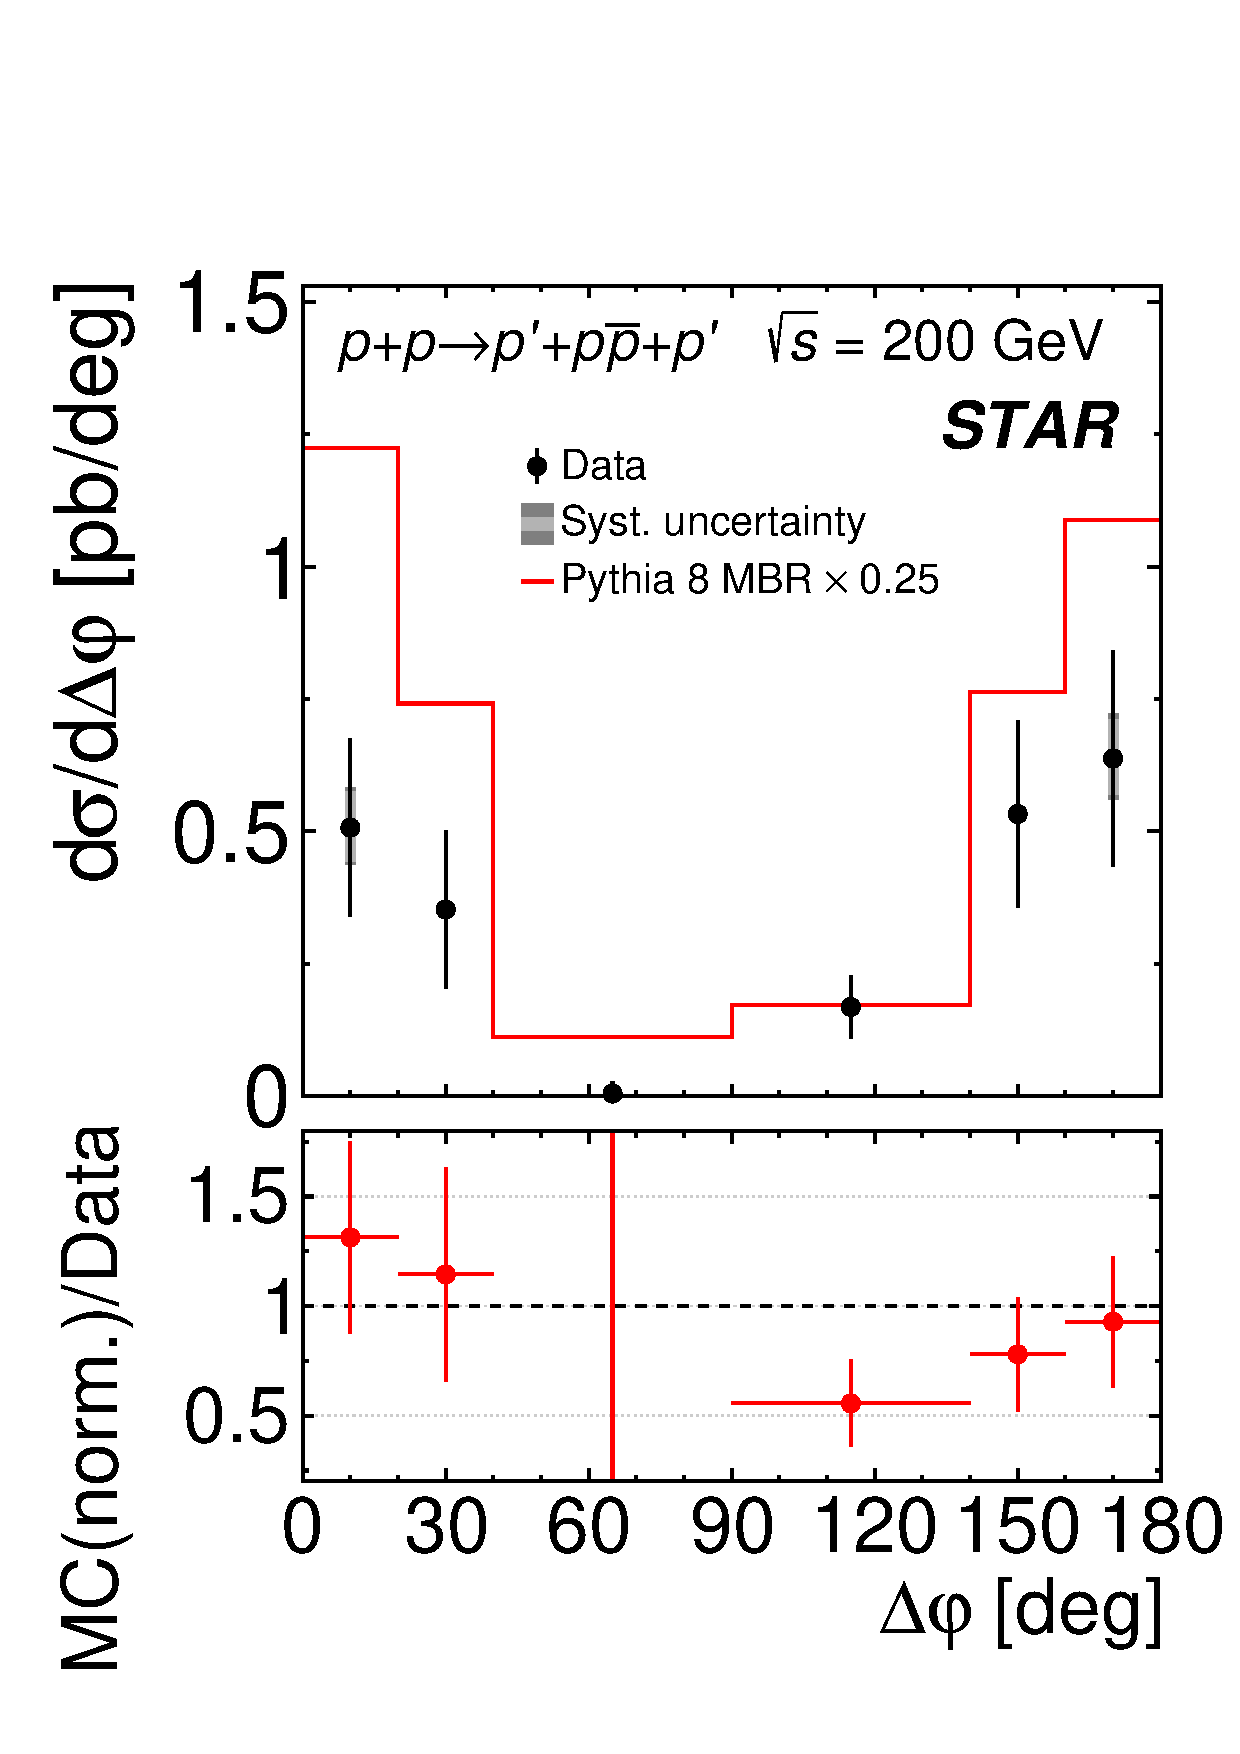
\includegraphics[width=.31\textwidth,page=1]{graphics/physicsResults/Ratio_FinalResult_DeltaPhi_proton.pdf}
\newline
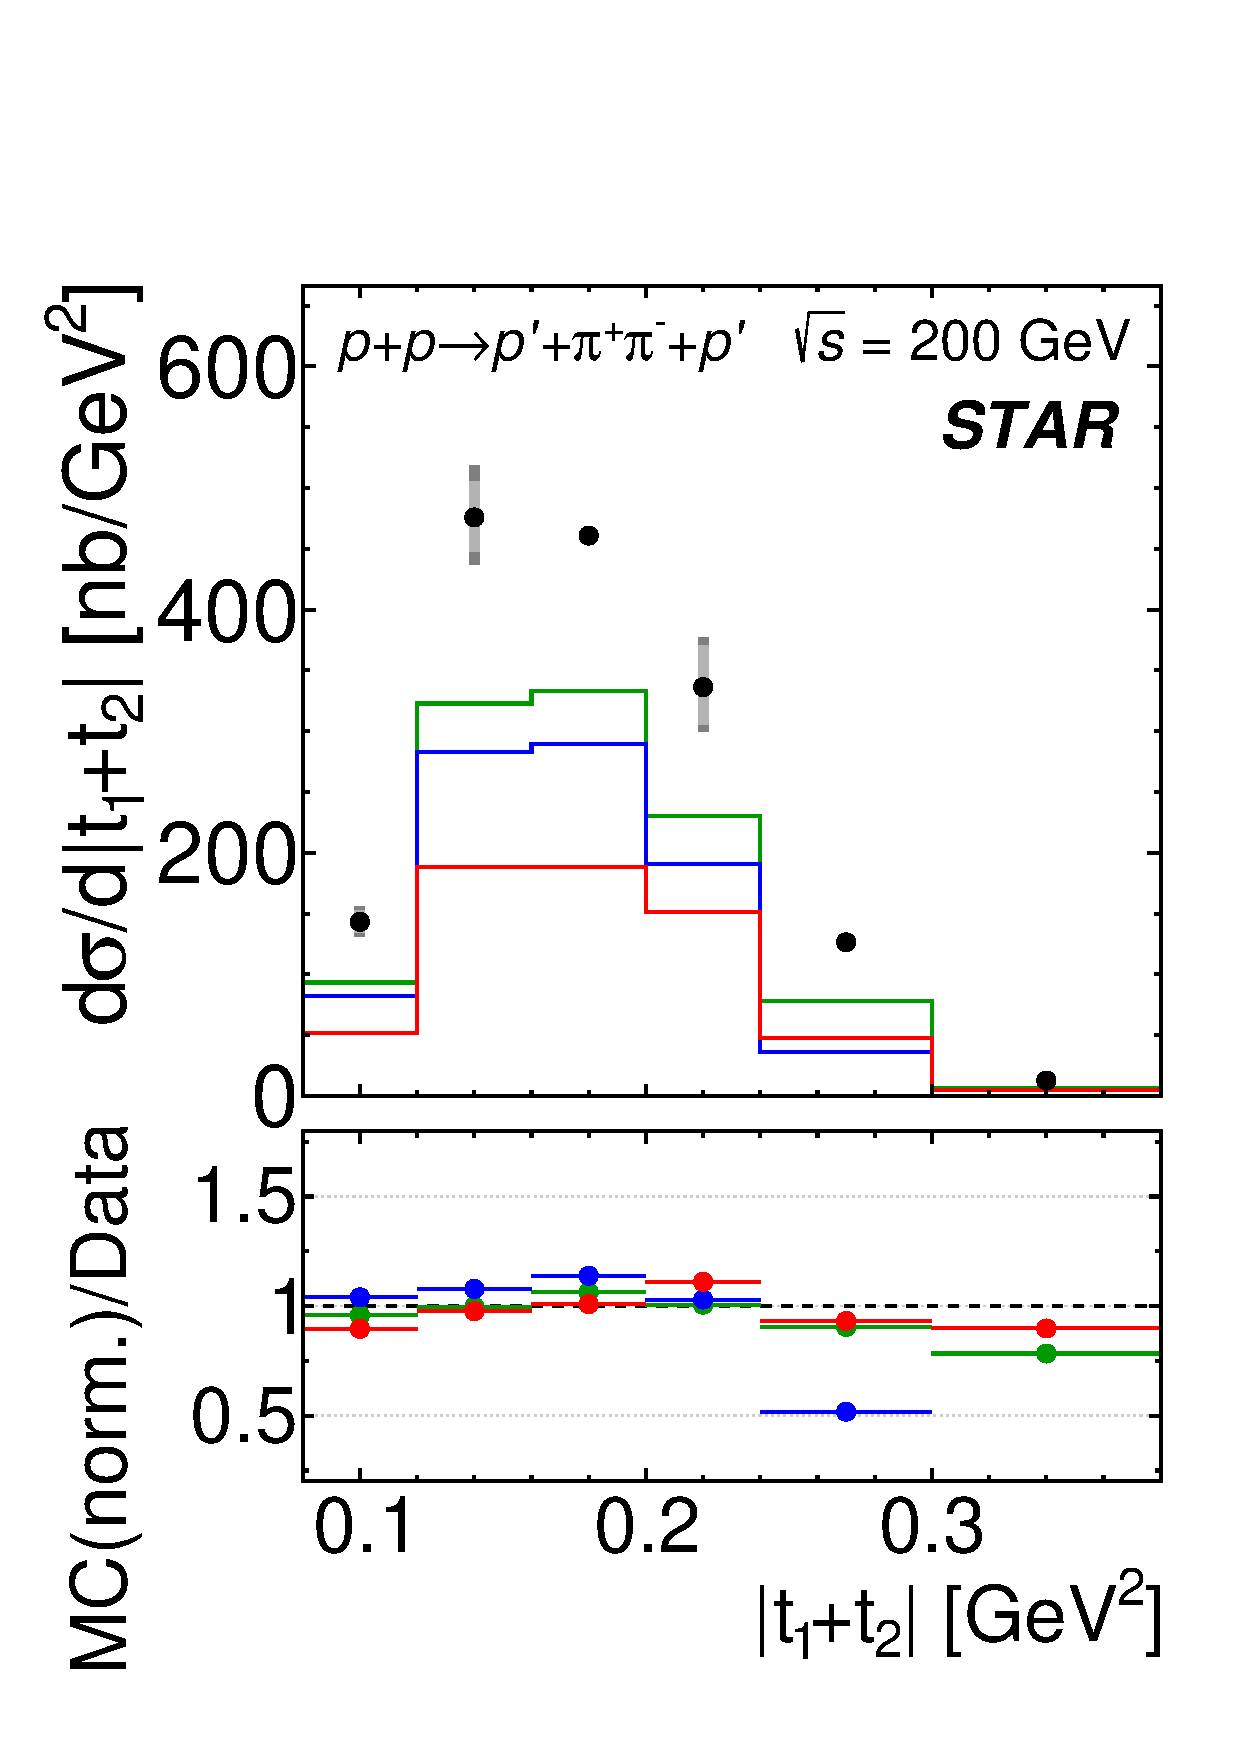
\includegraphics[width=.31\textwidth,page=1]{graphics/physicsResults/Ratio_FinalResult_MandelstamTSum_pion.pdf}
\hfill
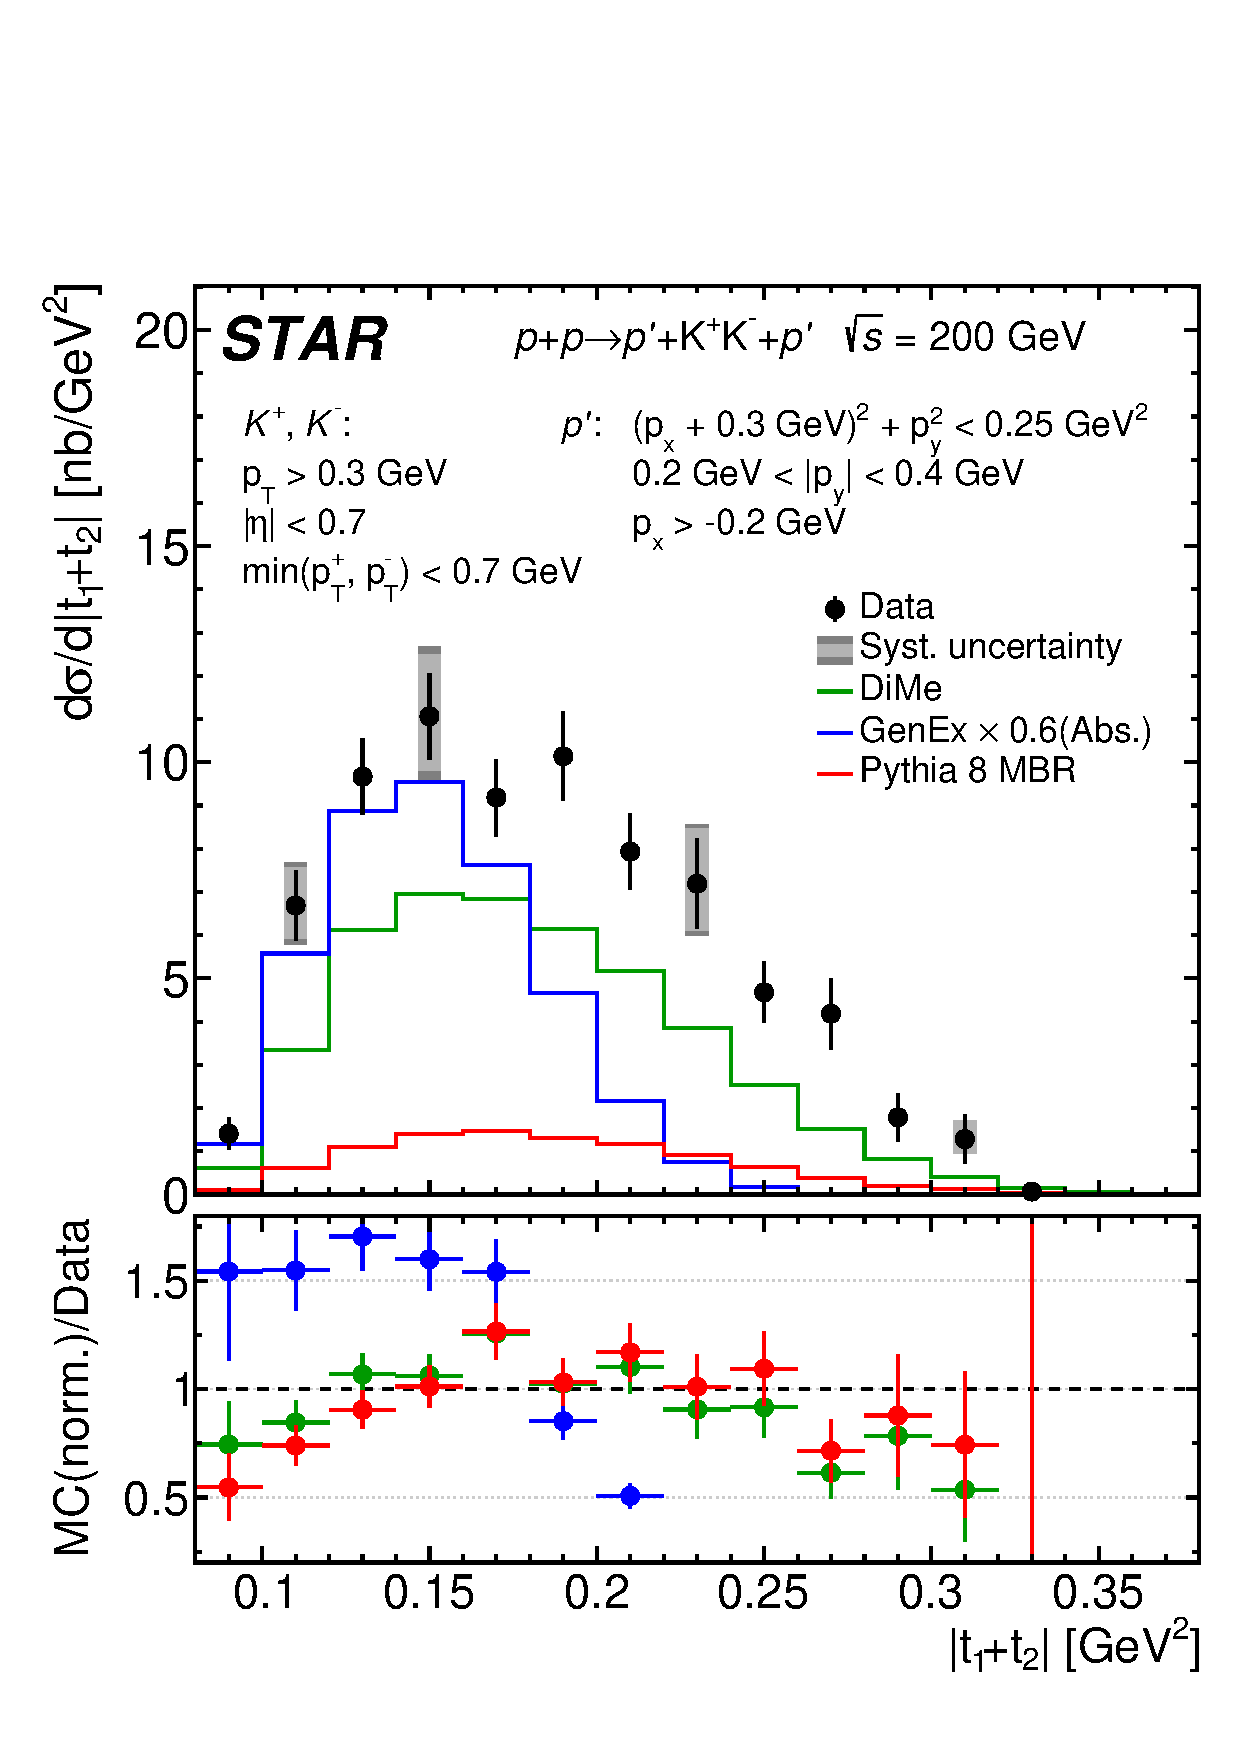
\includegraphics[width=.31\textwidth,page=1]{graphics/physicsResults/Ratio_FinalResult_MandelstamTSum_kaon.pdf}
\hfill
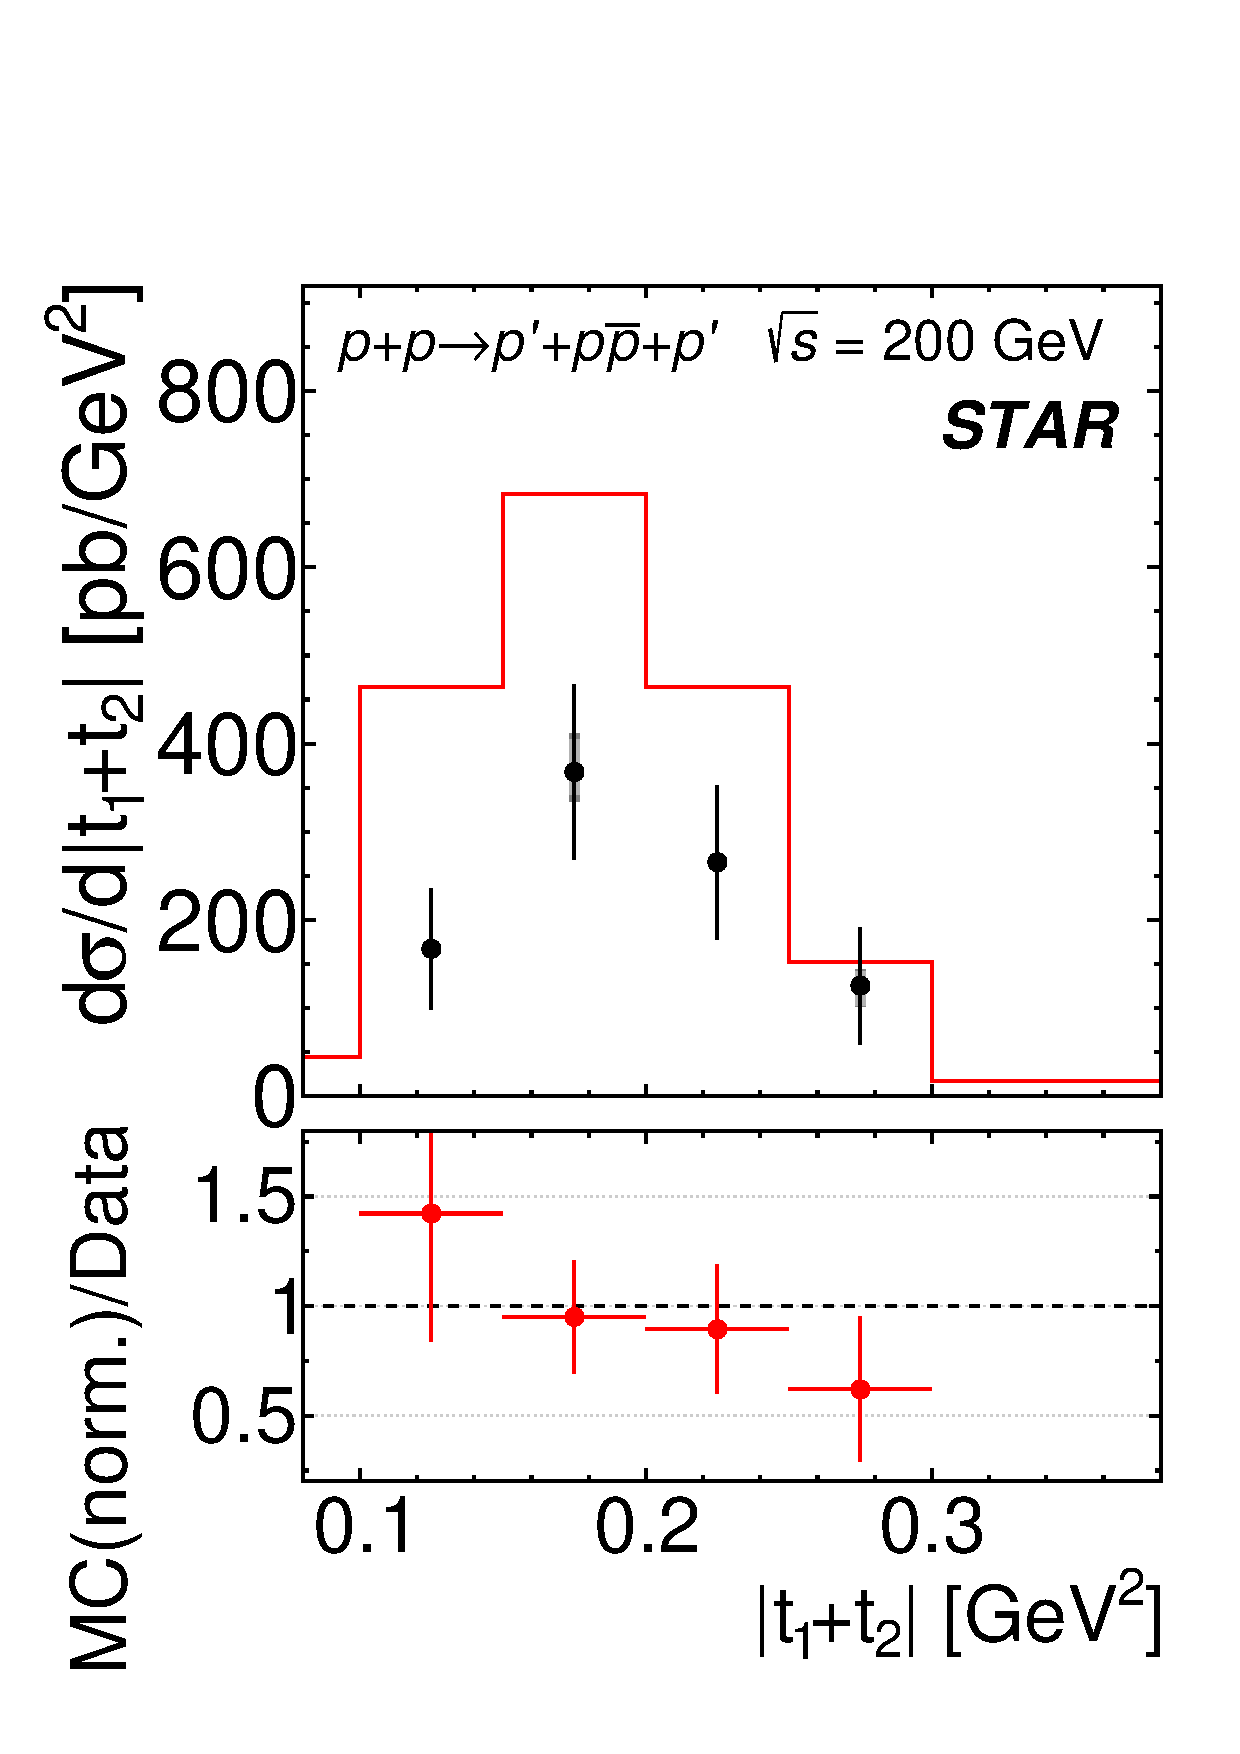
\includegraphics[width=.31\textwidth,page=1]{graphics/physicsResults/Ratio_FinalResult_MandelstamTSum_proton.pdf}
%
\caption[Differential cross sections for CEP of charged particle pairs $\pi^+\pi^-$, $K^+K^-$ and $p\bar{p}$ as a function of the difference of azimuthal angles of the forward scattered protons and of the sum of the squares of the four-momenta losses in the proton vertices measured in the fiducial region.]{Differential cross sections for CEP of charged particle pairs $\pi^+\pi^-$ (left column), $K^+K^-$ (middle column) and $p\bar{p}$ (right column) as a function of the difference of azimuthal angles of the forward scattered protons (top) and of the sum of the squares of the four-momenta losses in the proton vertices (bottom) measured in the fiducial region explained on the plots. Data are shown as solid points with error bars representing the statistical uncertainties. The typical systematic uncertainties are shown as gray boxes for only few data points as they are almost fully correlated between neighboring bins. Predictions from MC models GenEx, DiMe and MBR are shown as histograms. In the lower panels the ratios of the MC predictions scaled to data and the data are shown.}
\label{results_2}
\end{figure}
%
\begin{figure}[h]
\centering
\hspace*{5pt}
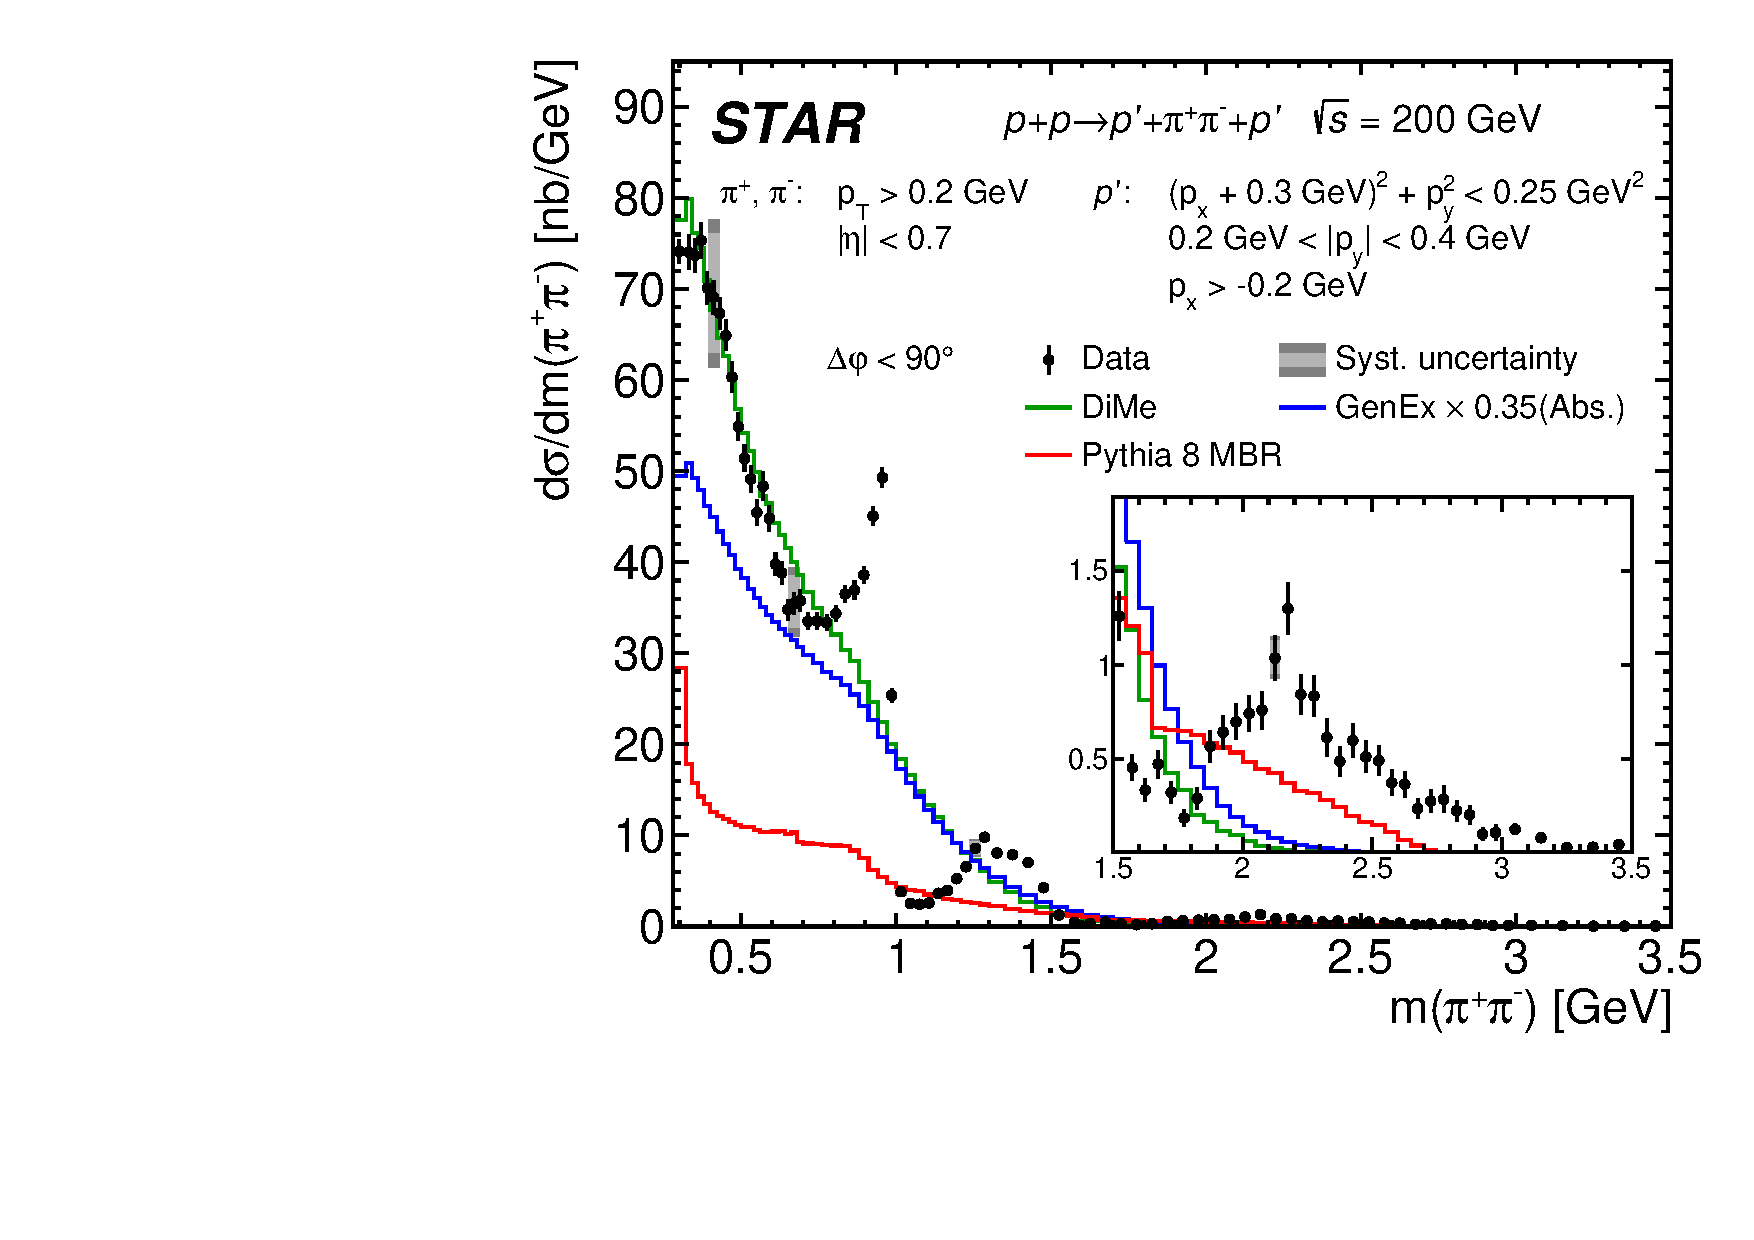
\includegraphics[width=.46\textwidth,page=1]{graphics/physicsResults/FinalResult_InvMass_DeltaPhiBin1_pion.pdf}
\hfill
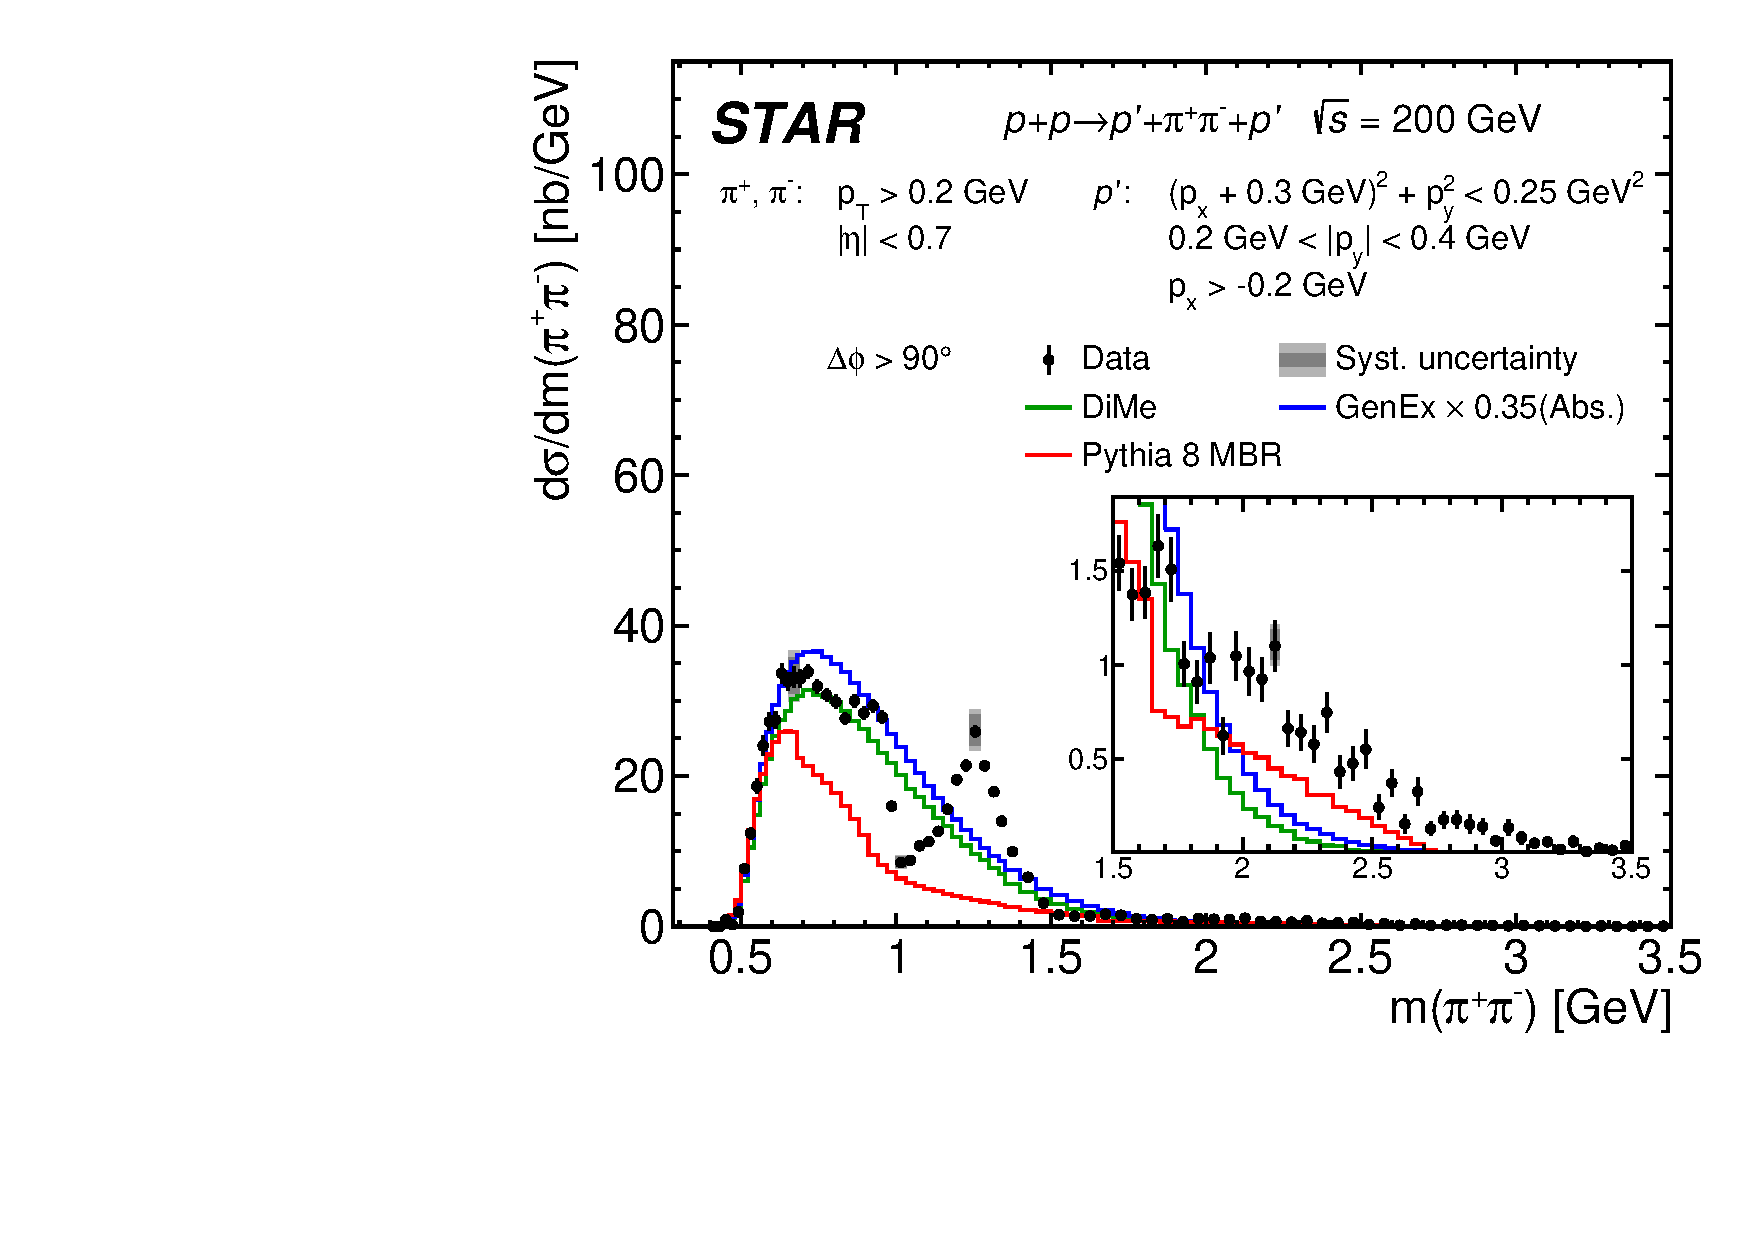
\includegraphics[width=.46\textwidth,page=1]{graphics/physicsResults/FinalResult_InvMass_DeltaPhiBin2_pion.pdf}
\hspace*{5pt}
\newline
\hspace*{5pt}
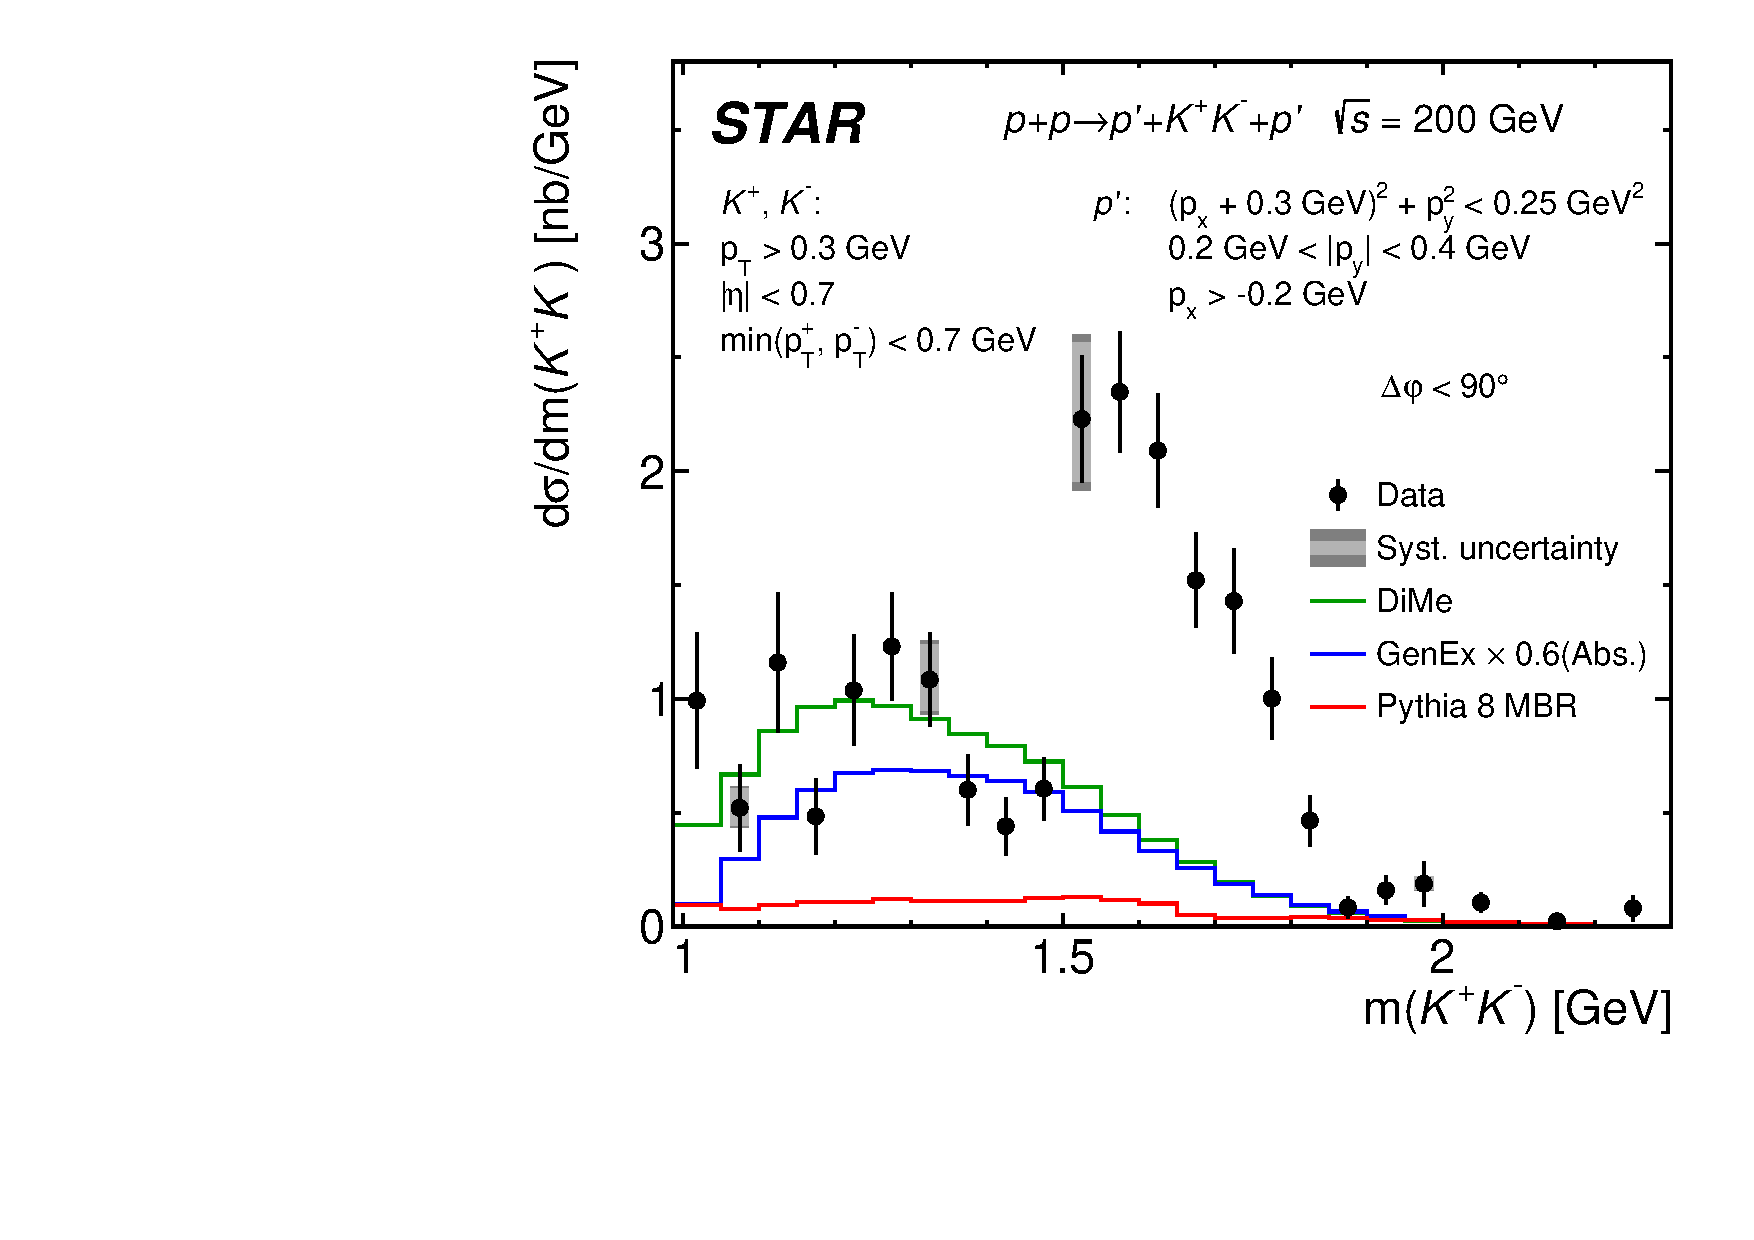
\includegraphics[width=.46\textwidth,page=1]{graphics/physicsResults/FinalResult_InvMass_DeltaPhiBin1_kaon.pdf}
\hfill
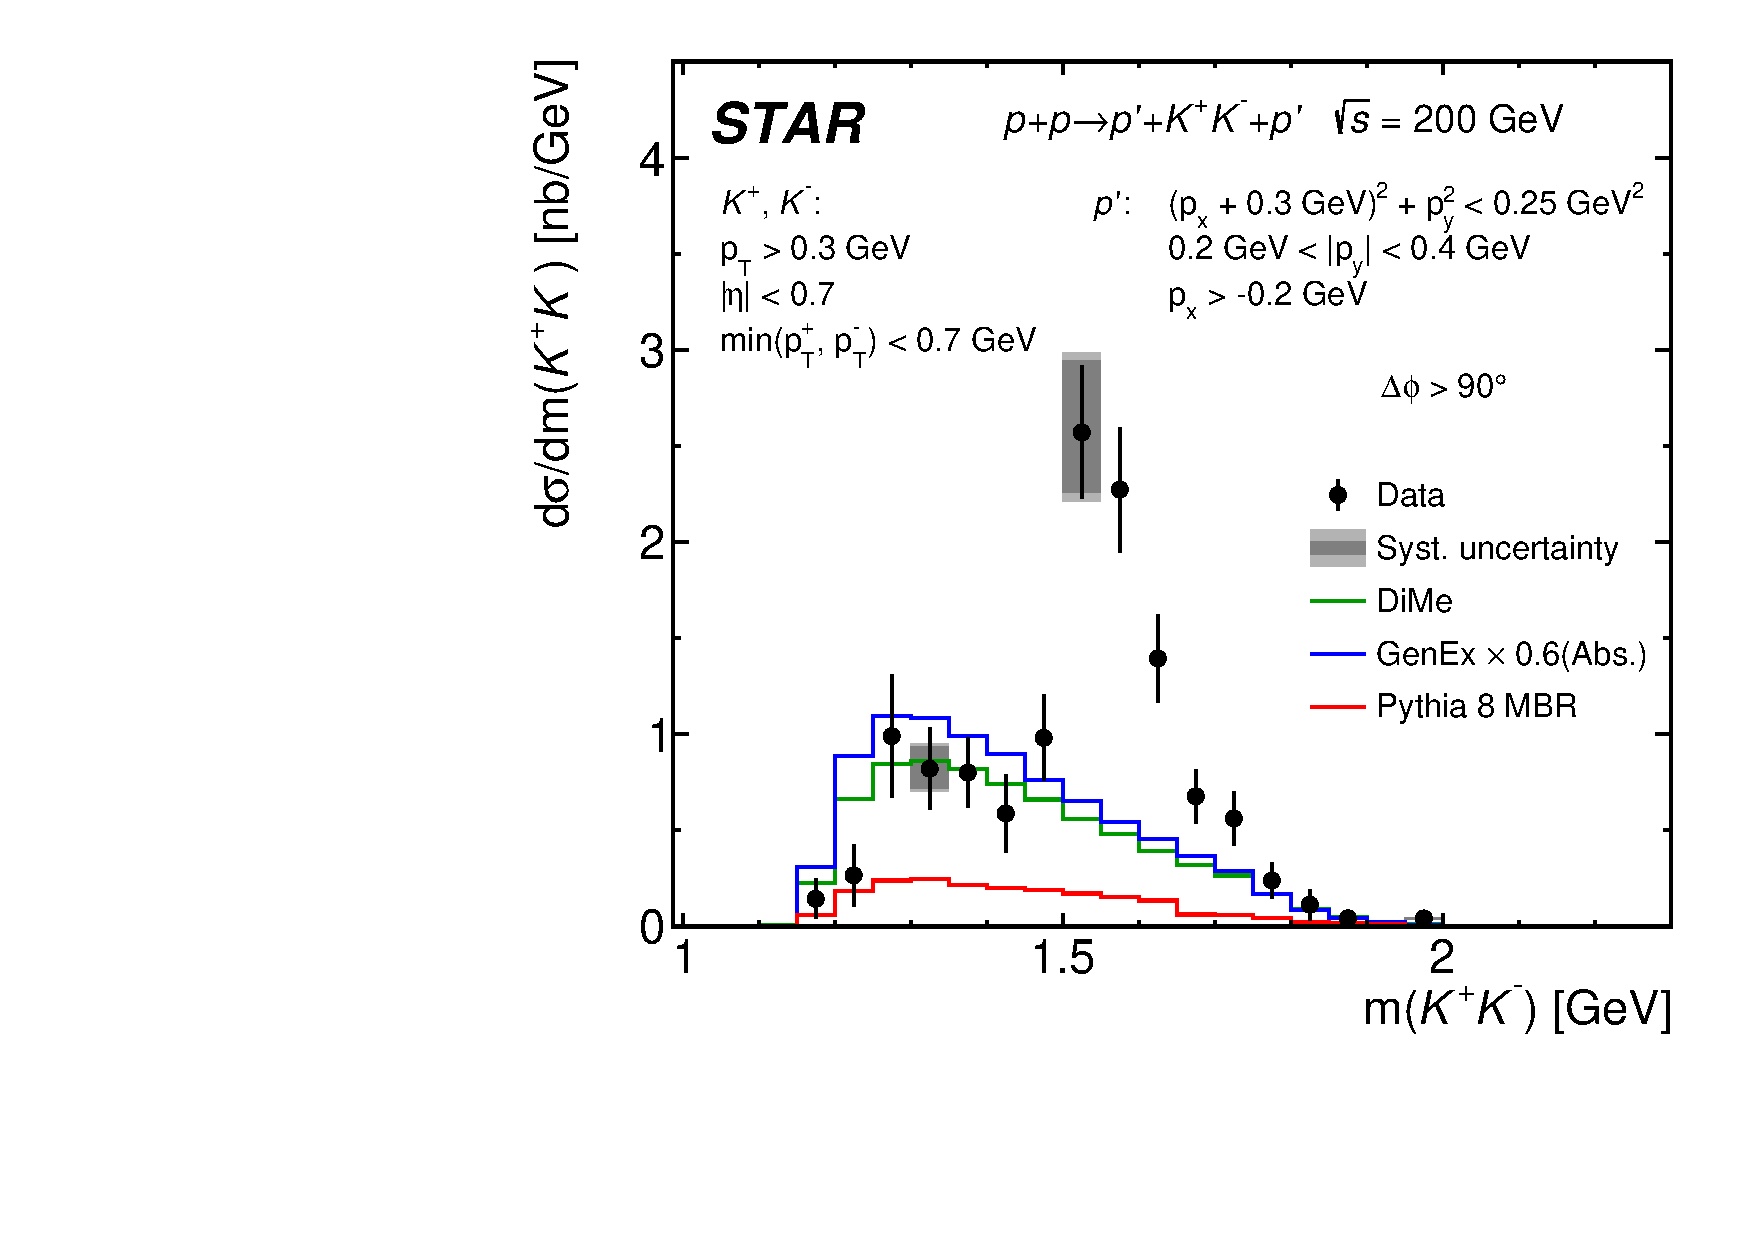
\includegraphics[width=.46\textwidth,page=1]{graphics/physicsResults/FinalResult_InvMass_DeltaPhiBin2_kaon.pdf}
\hspace*{5pt}
\newline
\hspace*{5pt}
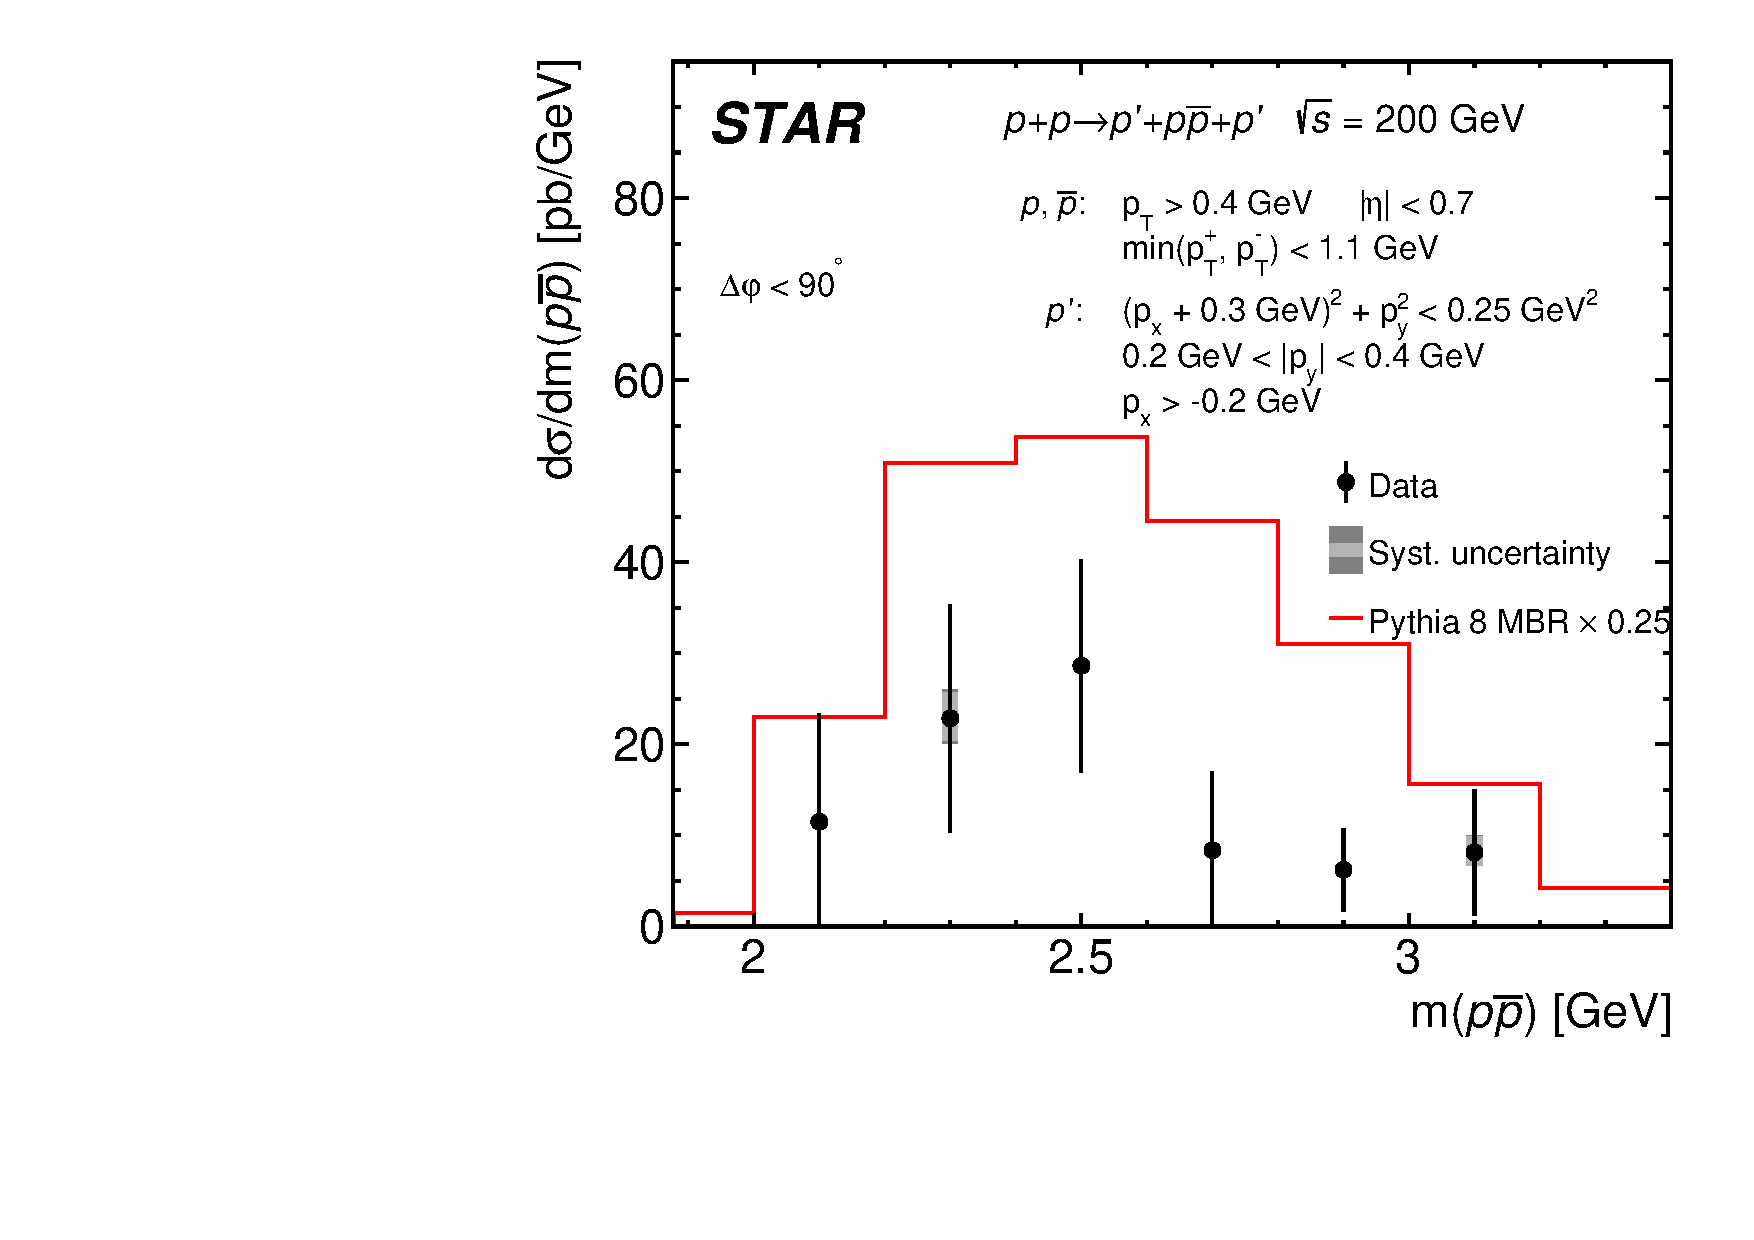
\includegraphics[width=.46\textwidth,page=1]{graphics/physicsResults/FinalResult_InvMass_DeltaPhiBin1_proton.pdf}
\hfill
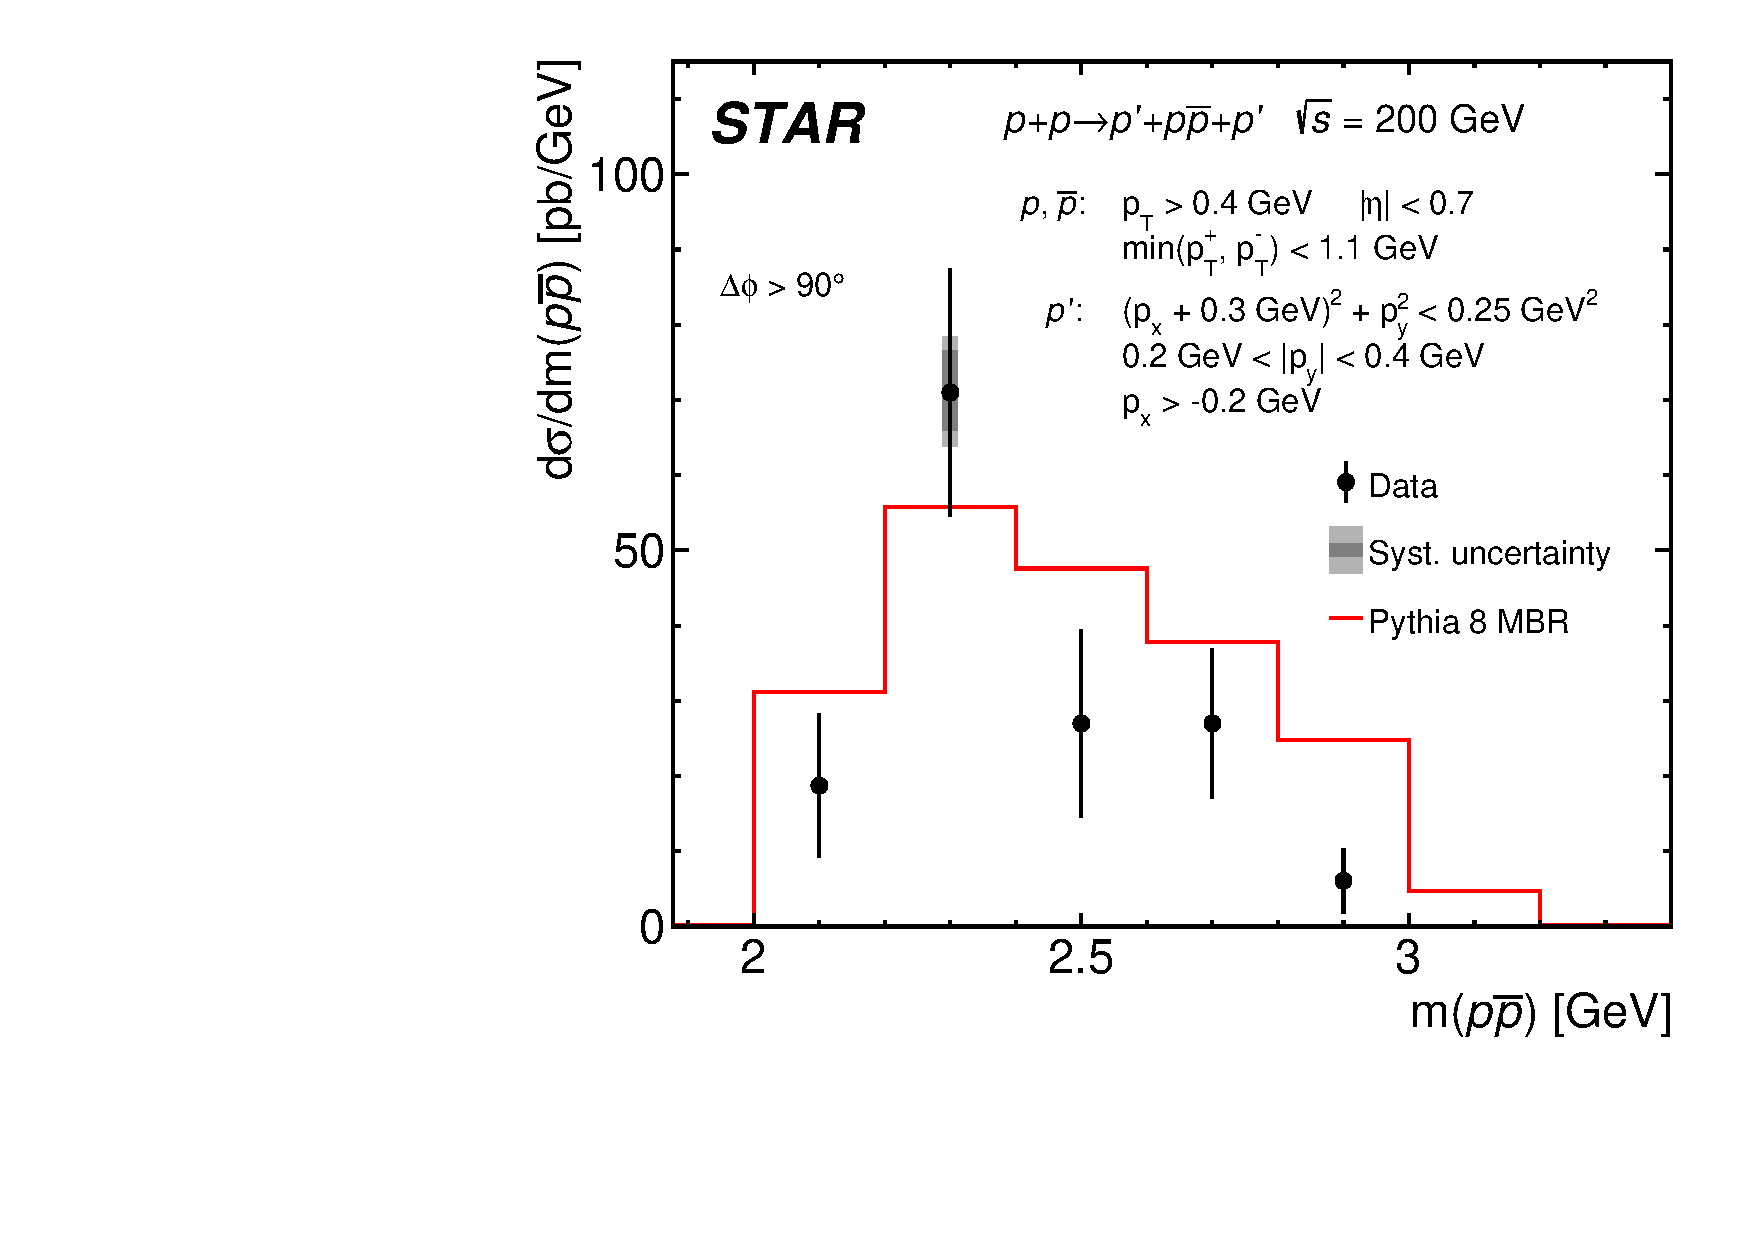
\includegraphics[width=.46\textwidth,page=1]{graphics/physicsResults/FinalResult_InvMass_DeltaPhiBin2_proton.pdf}
\hspace*{5pt}
%
\caption[Differential cross sections for CEP of charged particle pairs $\pi^+\pi^-$, $K^+K^-$ and $p\bar{p}$ as a function of the invariant mass of the pair in two $\Delta\phi$ regions: $\Delta\phi<90$ degree and $\Delta\phi>90$ degree  measured in the fiducial region explained on the plots.]{Differential cross sections for CEP of charged particle pairs $\pi^+\pi^-$ (top), $K^+K^-$ (middle) and $p\bar{p}$ (bottom) as a function of the invariant mass of the pair in two $\Delta\phi$ regions: $\Delta\phi<90$ degree (left column) and $\Delta\phi>90$ degree (right column) measured in the fiducial region explained on the plots. Data are shown as solid points with error bars representing the statistical uncertainties. The typical systematic uncertainties are shown as gray boxes for only few data points as they are almost fully correlated between neighboring bins. Predictions from MC models GenEx, DiMe and MBR are shown as histograms.}
\label{results_3}
\end{figure}



{
\renewcommand{\arraystretch}{1.5}
\begin{table}[]\centering
\begin{tabular}{cc c c}
~ & ~ & \multicolumn{2}{c}{$\bm{ \sigma_{\text{\bf{fid}}} \pm \delta_{\text{\bf{stat}}} \pm \delta_{\text{\bf{syst}}}}$} \\
 \bf{PID} & \bf{unit} & $\bm{\Delta\varphi<90^{\circ}}$ & $\bm{\Delta\varphi>90^{\circ}}$ \\ \hline\hline
 $\bm{\pi^{+}\pi^{-}}$ & \bf{nb} & $38.2\pm0.2^{+4.5}_{-3.9}$ & $18.5\pm0.1^{+2.0}_{-1.8}$ \\ %\hline
 $\bm{K^{+}K^{-}}$ & \bf{pb} & $971\pm50^{+160}_{-140}$ & $528\pm38^{+89}_{-78}$ \\ %\hline
 $\bm{p\bar{p}}$ & \bf{pb} & $16.2\pm4.1^{+3.0}_{-2.8}$ & $30.3\pm5.7^{+4.7}_{-4.3}$\\ %\hline%\hline
\end{tabular}
\caption{Integrated fiducial cross sections for CEP of $\pi^{+}\pi^{-}$, $K^{+}K^{-}$ and $p\bar{p}$ pairs in two ranges of azimuthal angle difference $\Delta\varphi$ between forward scattered protons. Statistical and systematic uncertainties are provided for each cross section.}\label{tab:xSec}
\end{table}
}


% %
% \FloatBarrier
% %
% Such correlation between resonances seen in mass spectrum and azimuthal angle between outgoing protons indicates factorization breaking between the two proton vertices. In the range $\Delta\phi<$ 90 degrees the DiMe model well describes both normalization and shape of mass spectrum at $m(\pi^+\pi^-)<$ 0.5 GeV.
% %
% In case of the cross section for CEP of $K^+K^-$ pairs the data do not show any significant asymmetry except possible widening
% of the peak at $f_2^\prime(1520)$ in the region $\Delta\phi<90$ degrees which may indicate an enhancement of additional resonances around 1.7~GeV in this configuration.
% %
% In case of the cross section for CEP of $p\bar{p}$ pairs data do not show any significant asymmetry except possible enhancement in the $2.2-2.4$ mass range for the $\Delta\phi>90$ degrees region.\\
% %
% \indent
% Due to high statistics of the two-pion sample it is possible to study the CEP of $\pi^+\pi^-$ pairs in more detail.
% Figure~\ref{results_4} shows the differential cross sections for CEP of $\pi^+\pi^-$ pairs as a function of the pair rapidity (left column), $\Delta\phi$ (middle column) and $|t_1+t_2|$ (right column) in three characteristic ranges of the invariant mass of the pair: $m(\pi^+\pi^-)<1.0$ GeV (mainly non-resonant production), $1.0< m(\pi^+\pi^-) <1.5$ GeV ($f_2(1270)$ mass range) and $m(\pi^+\pi^-)>1.5$ GeV (higher invariant masses).\\
% %
% \noindent
% Figure~\ref{results_4} shows the differential cross sections for CEP of different particle species pairs as a function of the pair rapidity (left column), of the difference of forward protons azimuthal angles (middle column) and of the sum of squares of the four-momenta transfers at the proton vertices (right column), for the three invariant mass ranges. In the case of the cross section $d\sigma/dy$ all models agree in shape with data in all three mass ranges except for the GenEx and DiMe predictions in the highest mass range where predictions is narrower.
% 
% Strong suppression of the fiducial cross section close to $90^\circ$ is due to the STAR RP acceptance while asymmetry $0^\circ$ vs. $180^\circ$ in the lowest mass region is due to the STAR TPC acceptance. $\Delta\phi$ distribution is sensitive to absorption  which are treated fully differentialy in DiMe generator and only on average in GenEx. This is consistent with generally better agreement between data and DiMe expectations except $f_2(1270)$ mass region. MBR model predicts symmetric $\Delta\phi$ distributions in all mass ranges which is not supported by the data.
% 
% The slope of the cross section as the function of $|t_1+t_2|$ is less steep in the $f_2(1270)$ mass region compared to other mass regions. In the low mass region the DiMe prediction has steeper slope compared to data.\\
%
\begin{figure}[h]
\centering
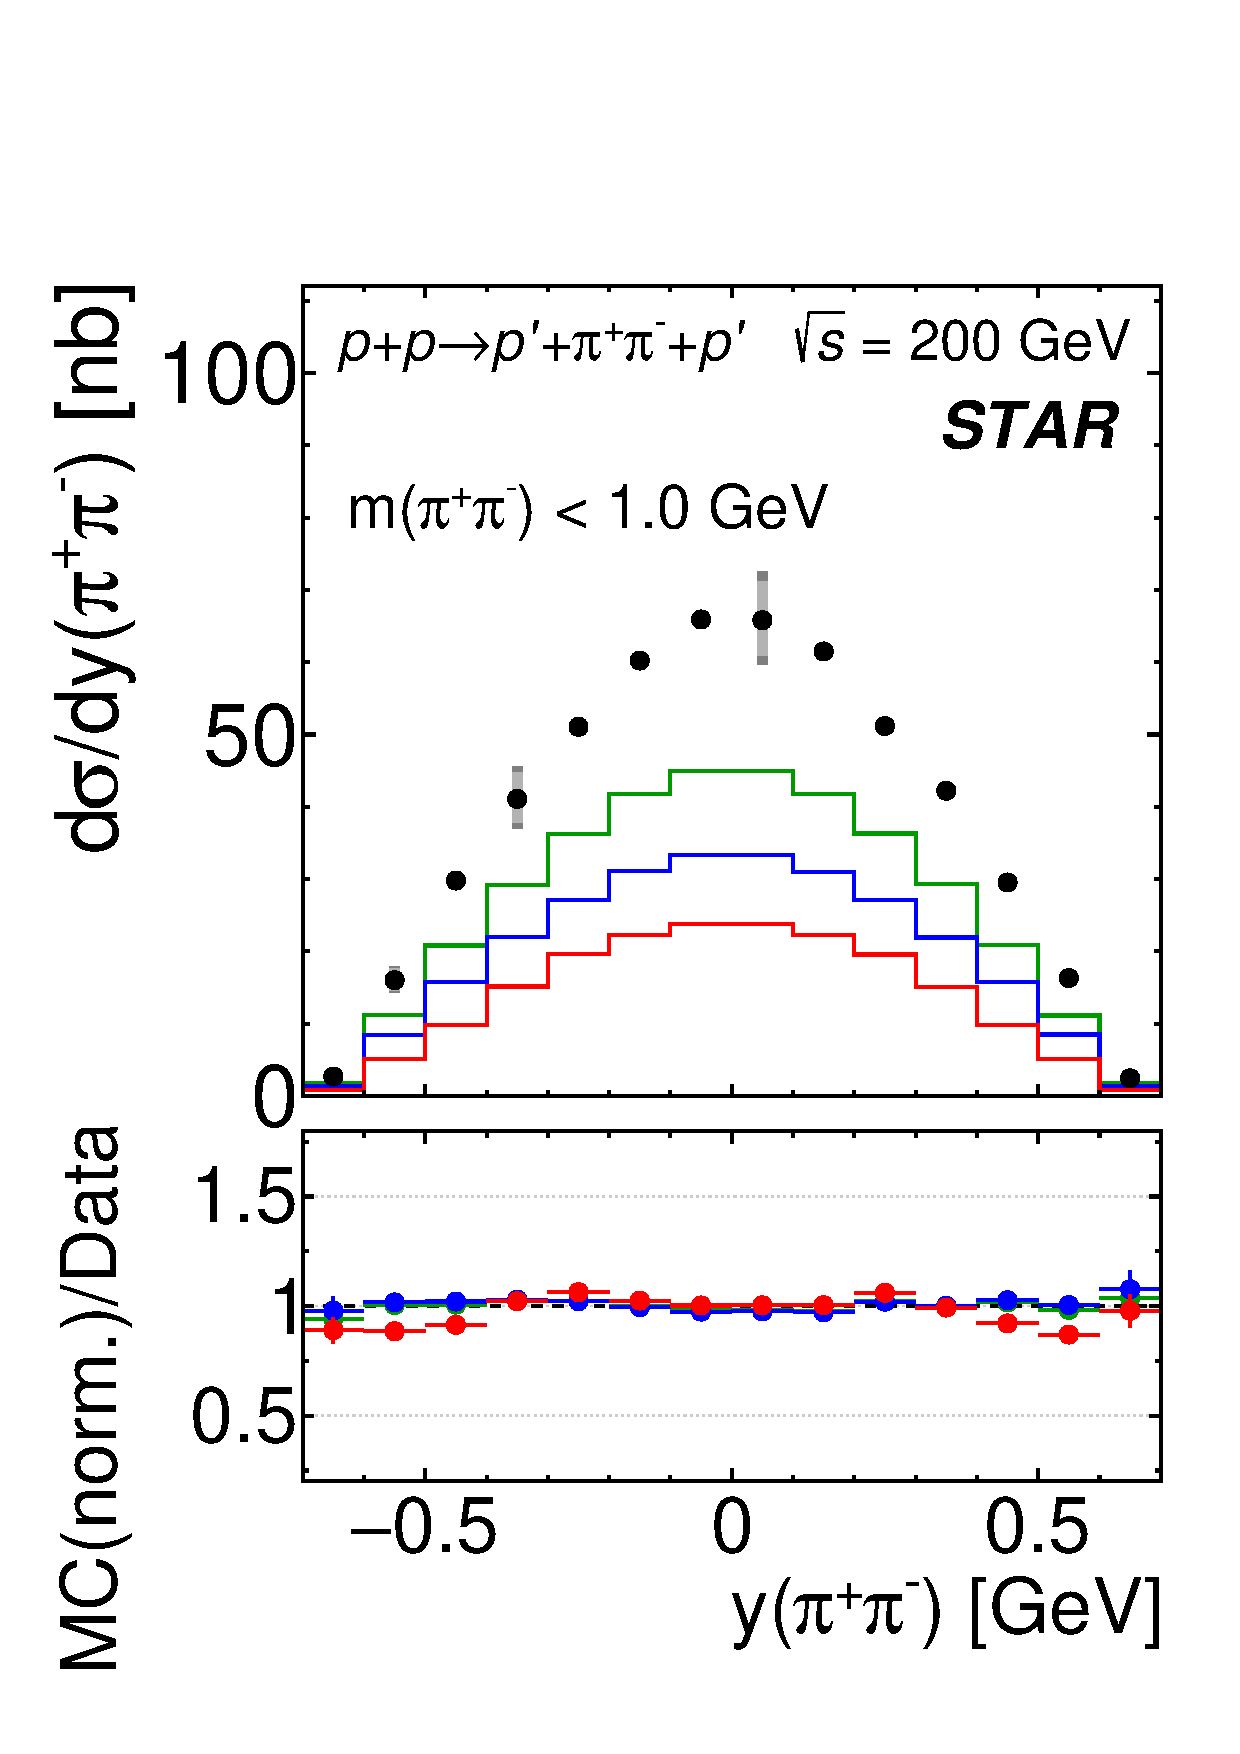
\includegraphics[width=.31\textwidth,page=1]{graphics/physicsResults/Ratio_FinalResult_Rapidity_pion_MassBin_1.pdf}
\hfill
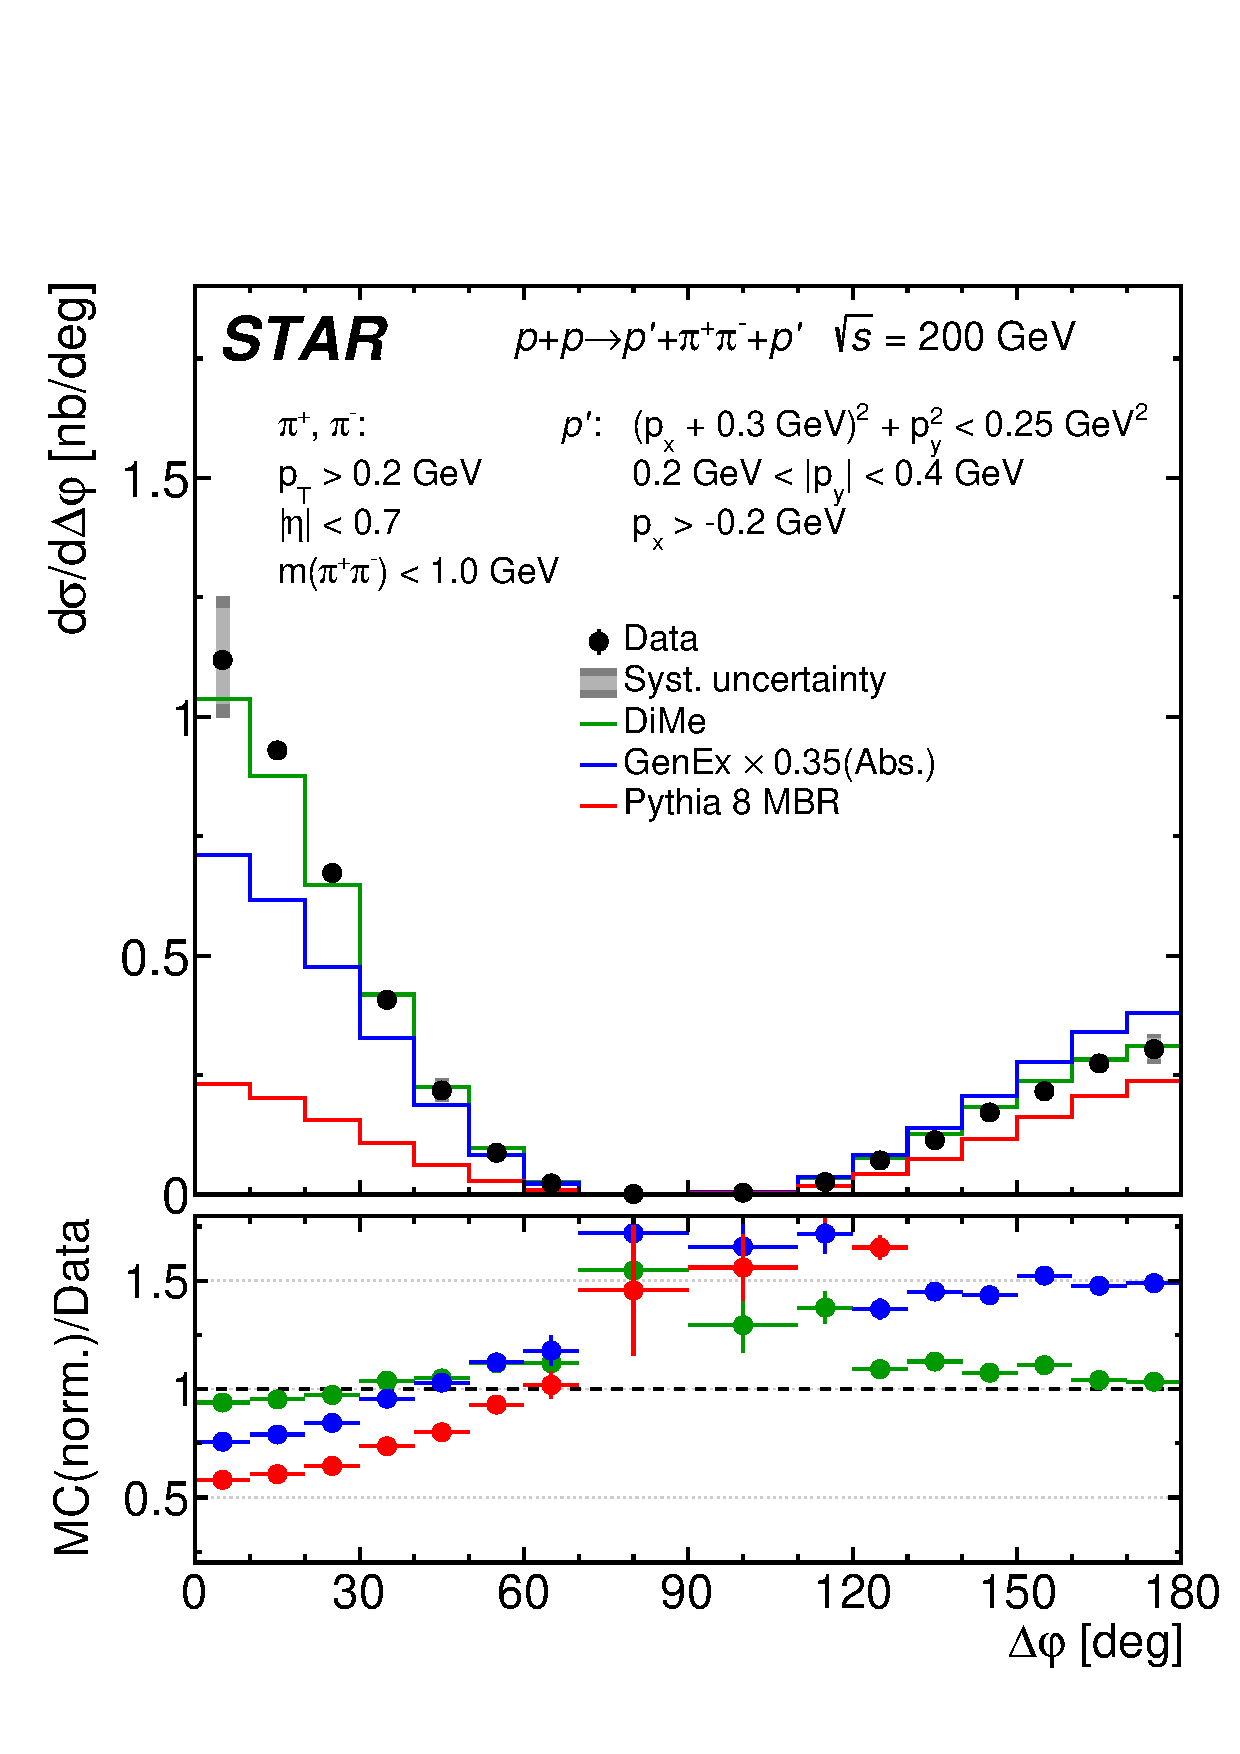
\includegraphics[width=.31\textwidth,page=1]{graphics/physicsResults/Ratio_FinalResult_DeltaPhi_pion_MassBin_1.pdf}
\hfill
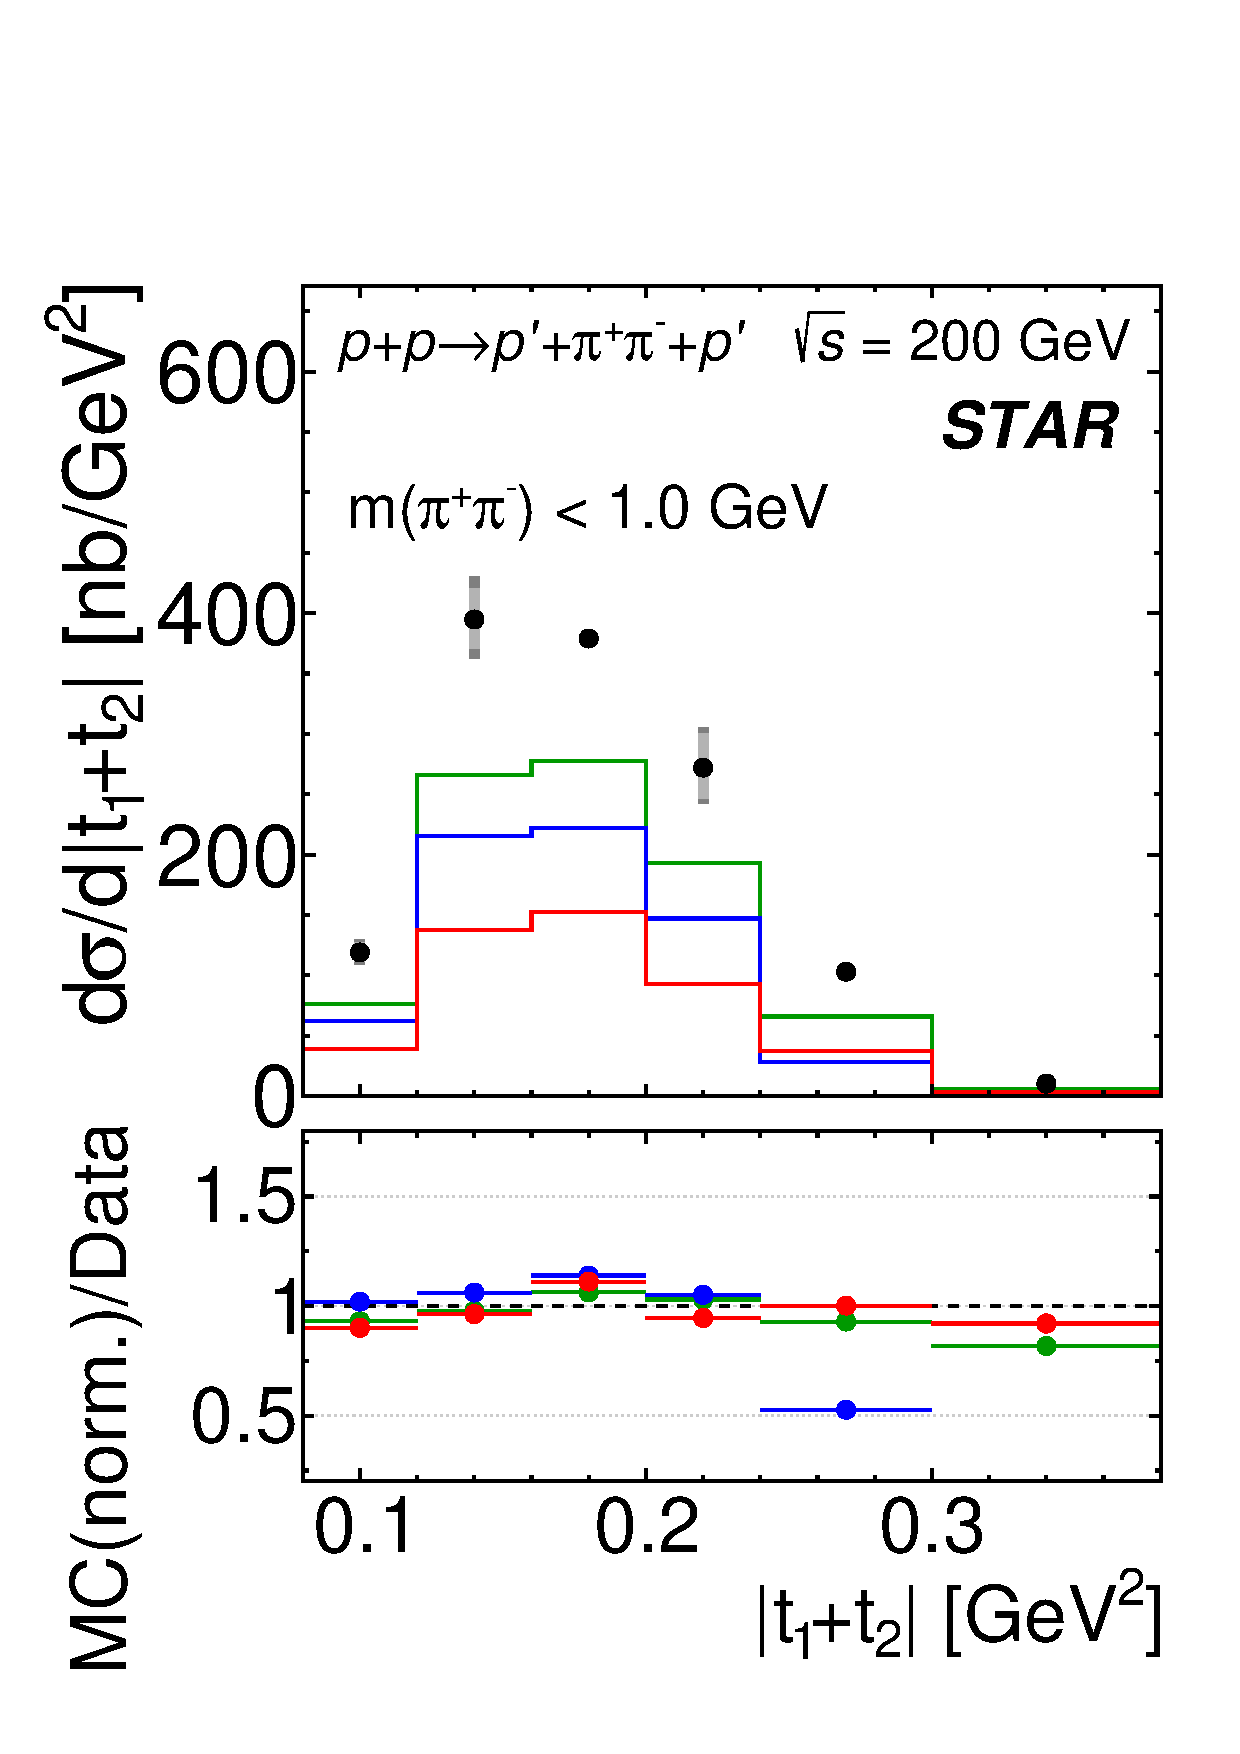
\includegraphics[width=.31\textwidth,page=1]{graphics/physicsResults/Ratio_FinalResult_MandelstamTSum_pion_MassBin_1.pdf}
\newline
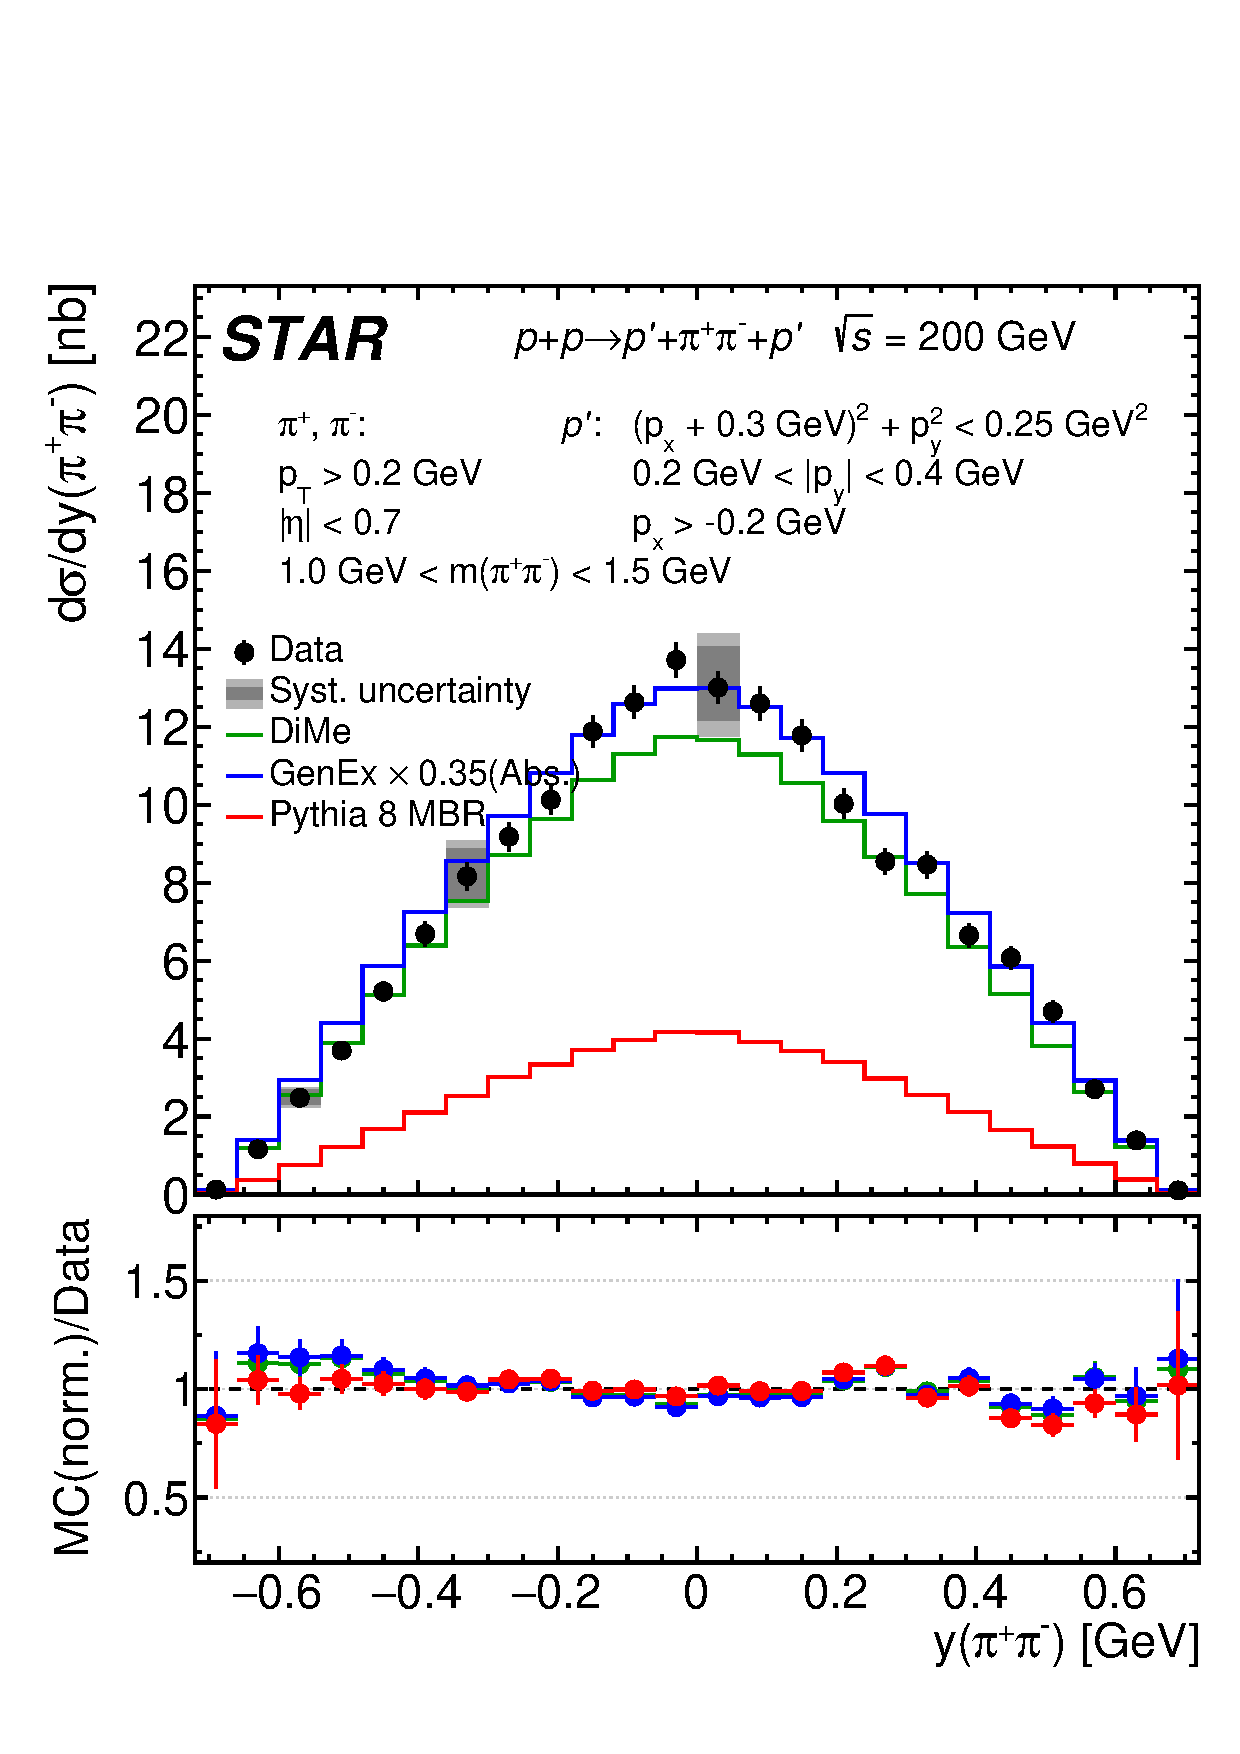
\includegraphics[width=.31\textwidth,page=1]{graphics/physicsResults/Ratio_FinalResult_Rapidity_pion_MassBin_2.pdf}
\hfill
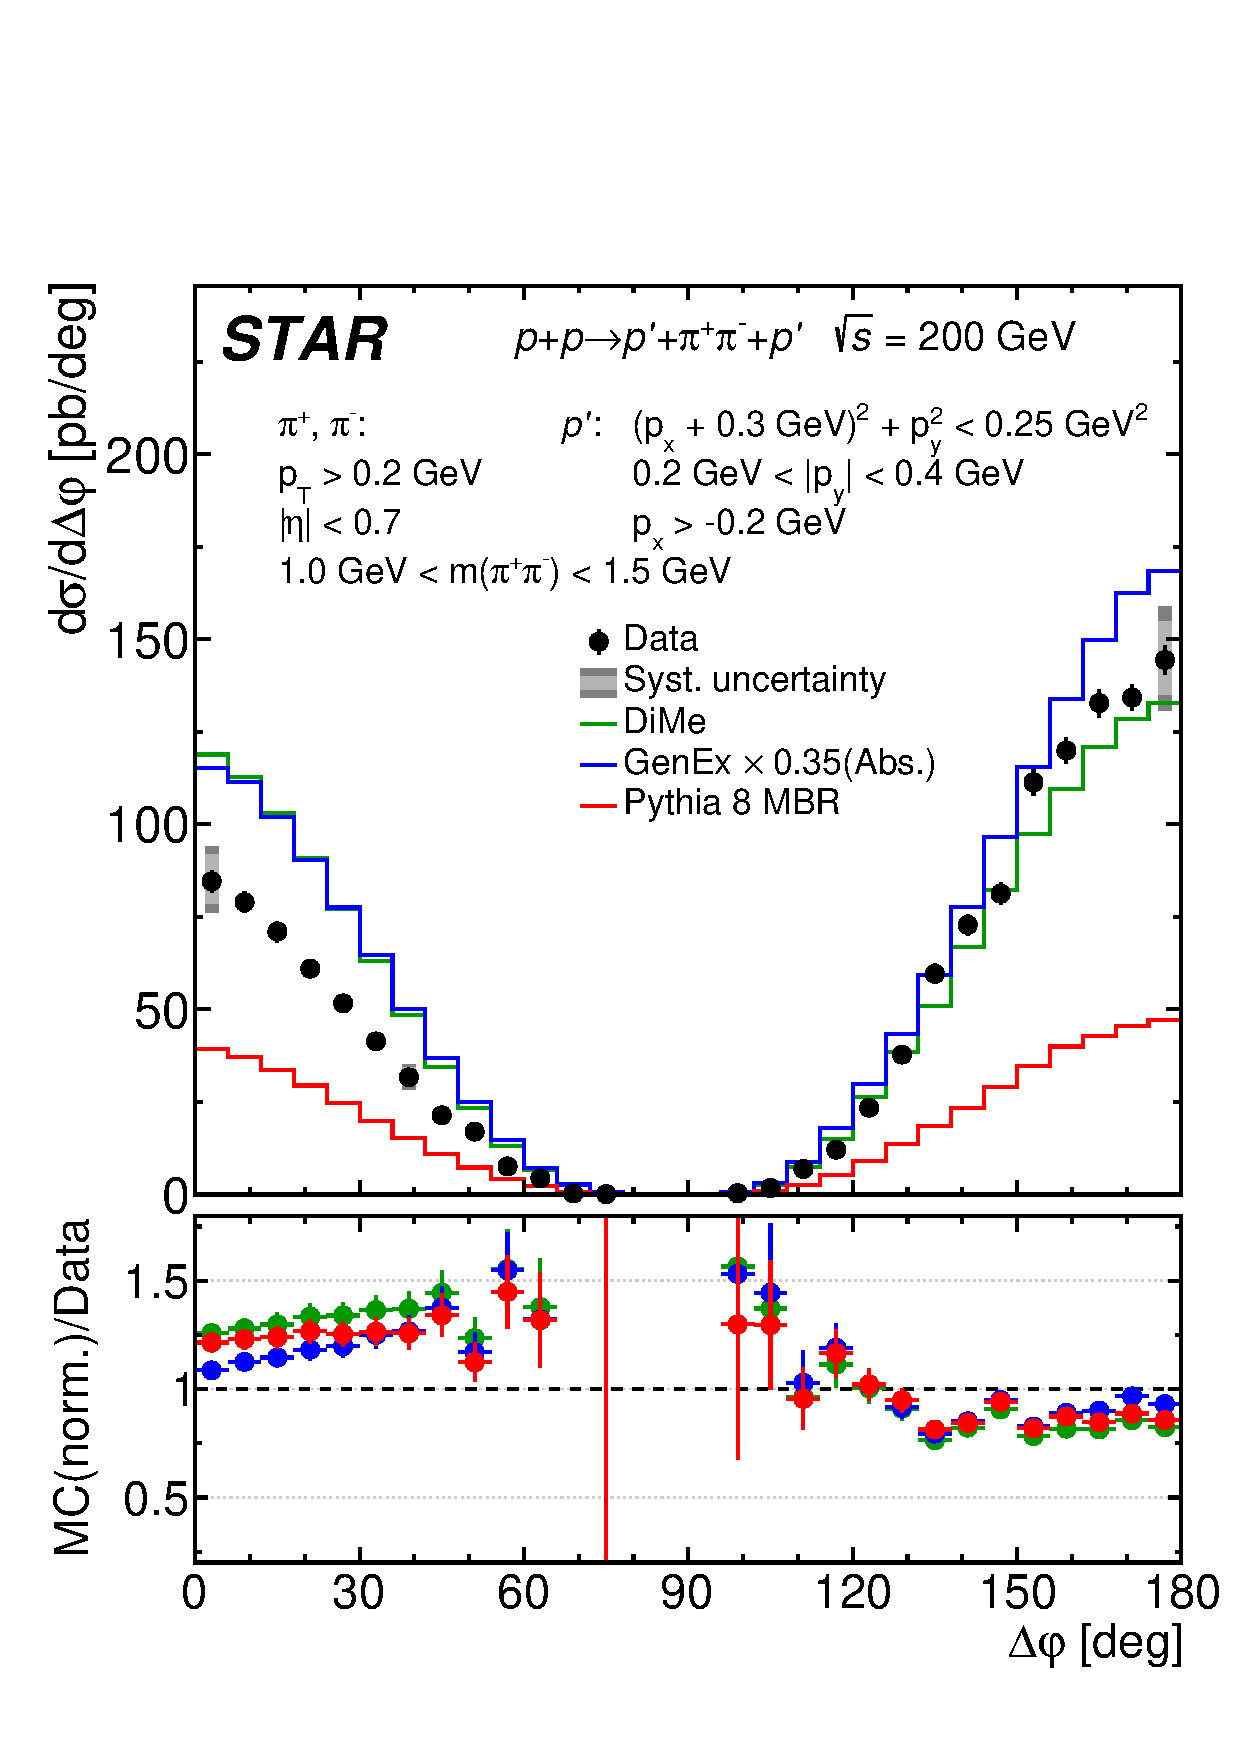
\includegraphics[width=.31\textwidth,page=1]{graphics/physicsResults/Ratio_FinalResult_DeltaPhi_pion_MassBin_2.pdf}
\hfill
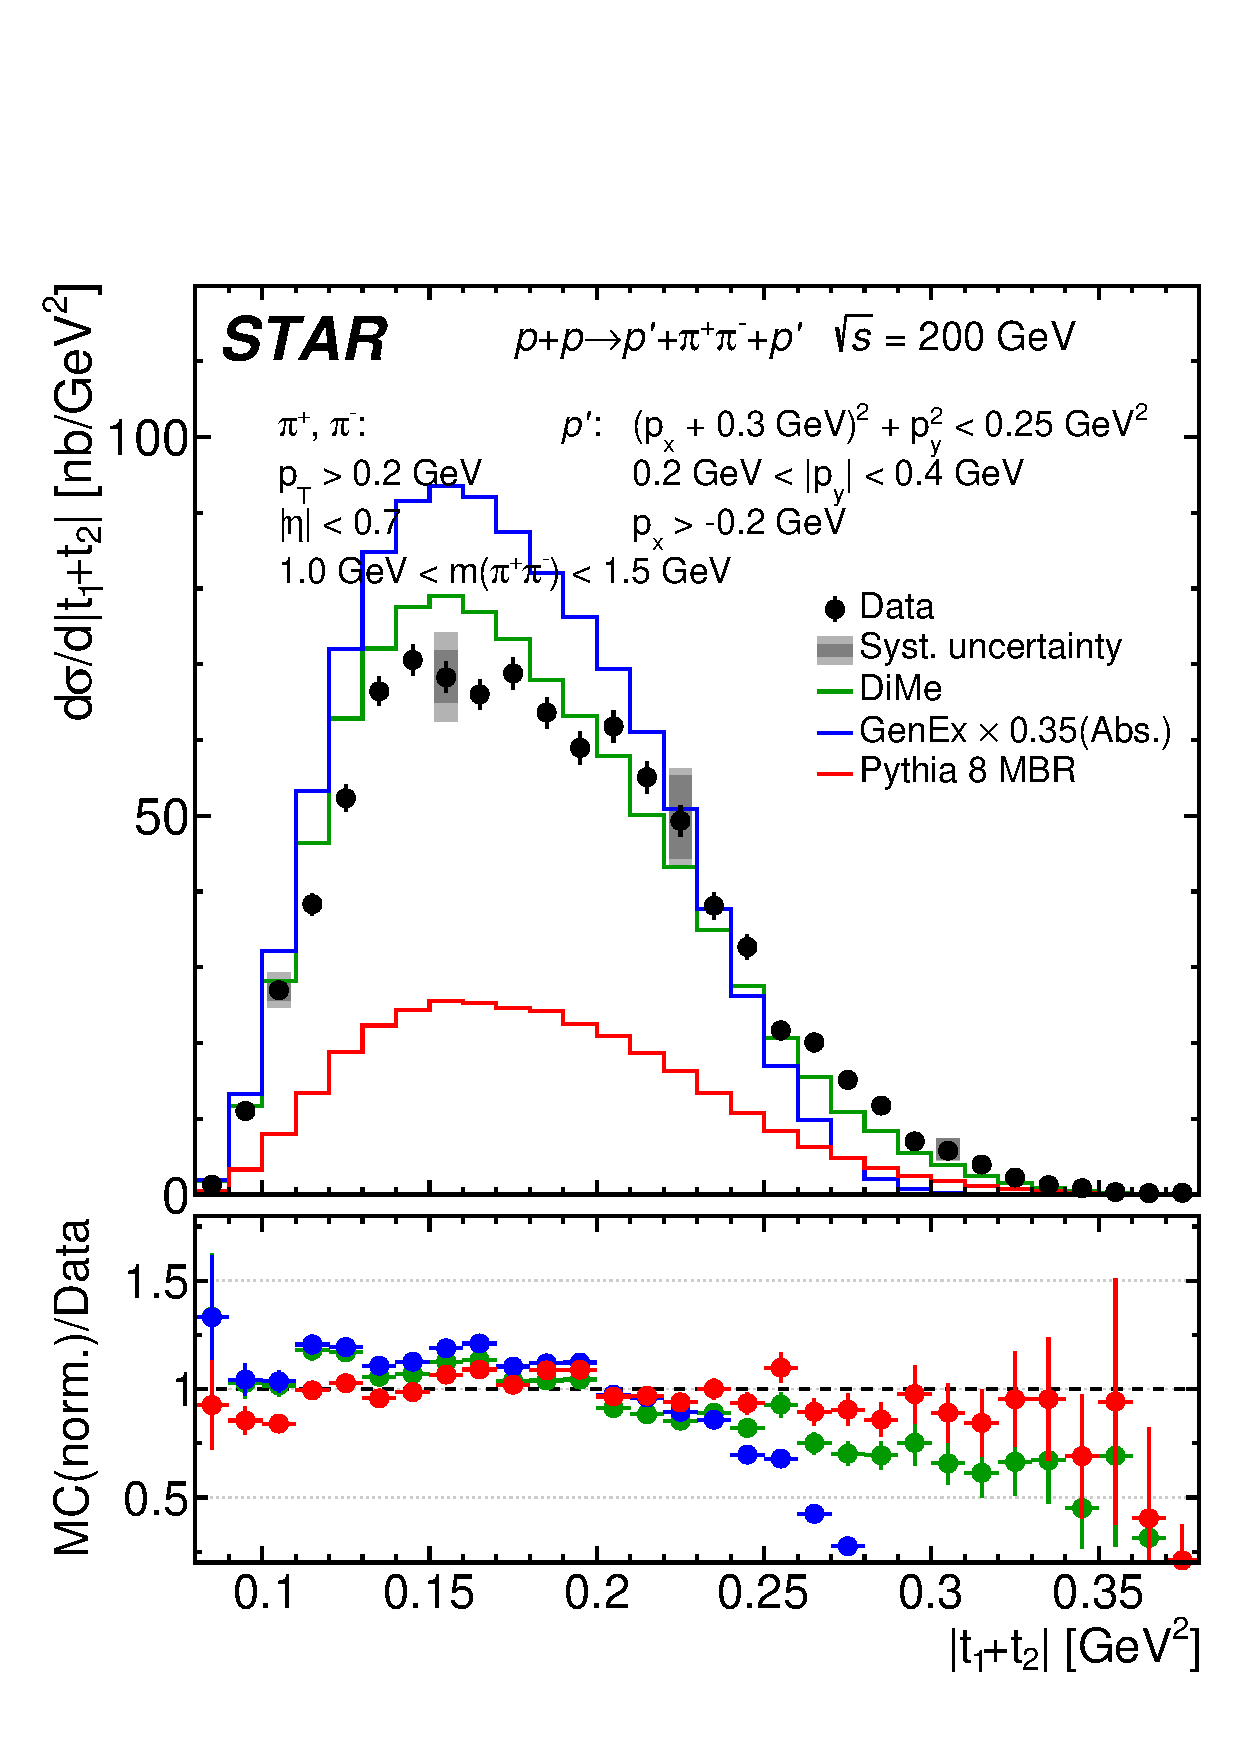
\includegraphics[width=.31\textwidth,page=1]{graphics/physicsResults/Ratio_FinalResult_MandelstamTSum_pion_MassBin_2.pdf}
\newline
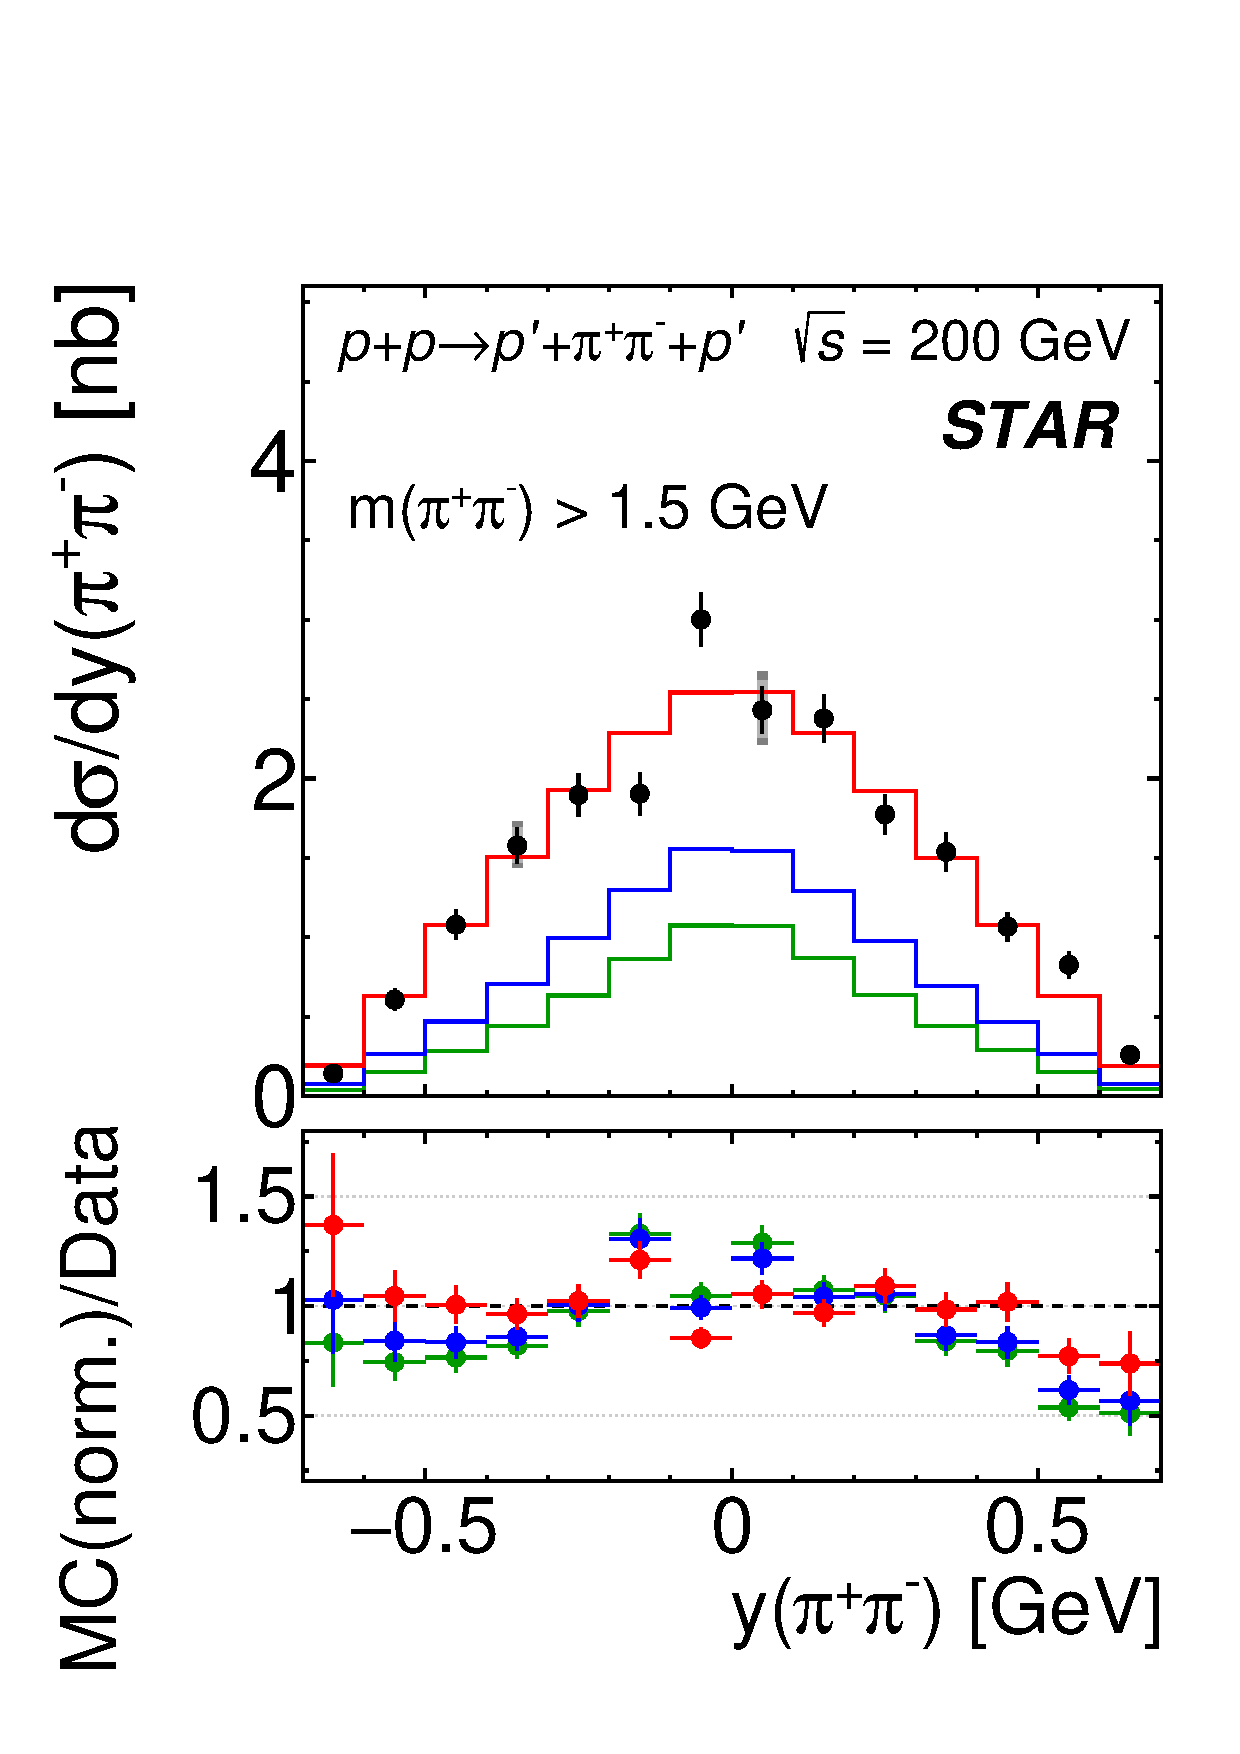
\includegraphics[width=.31\textwidth,page=1]{graphics/physicsResults/Ratio_FinalResult_Rapidity_pion_MassBin_3.pdf}
\hfill
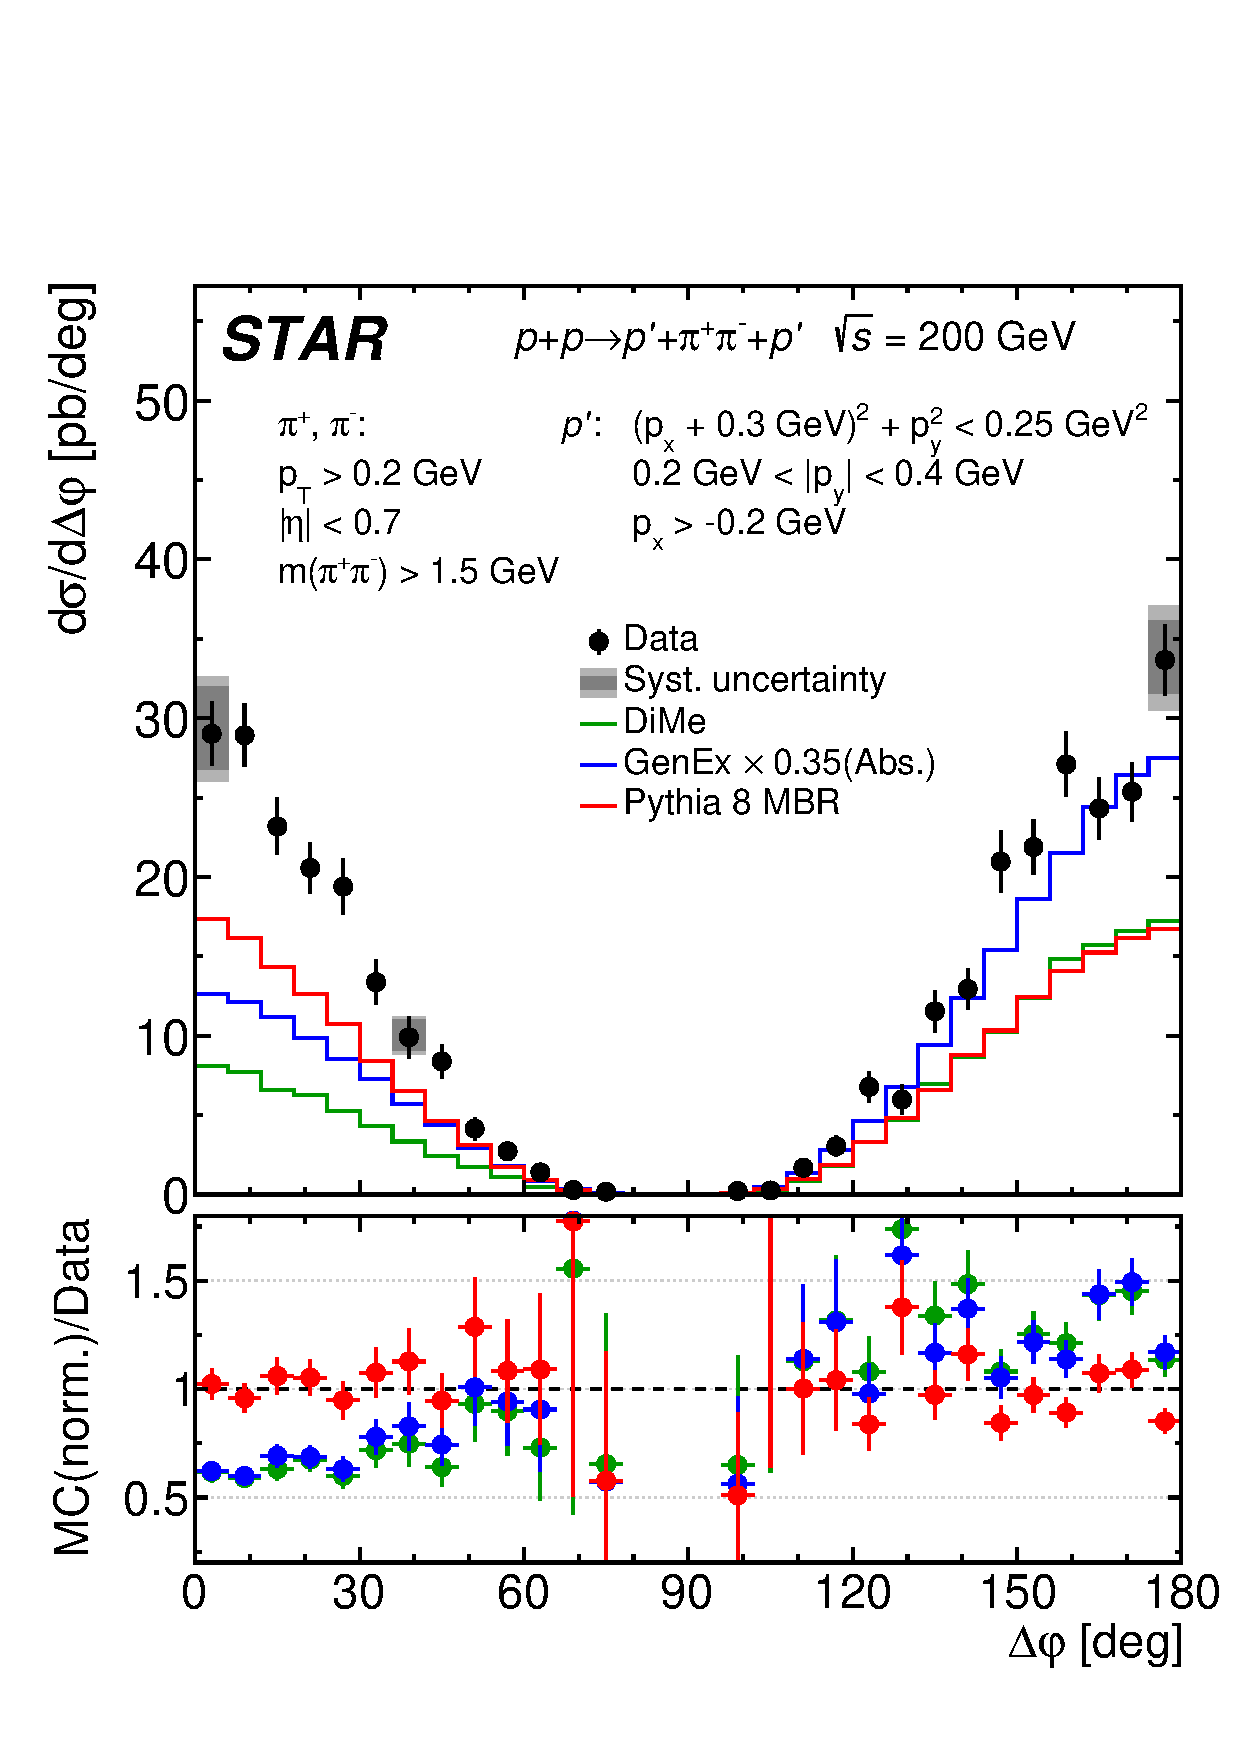
\includegraphics[width=.31\textwidth,page=1]{graphics/physicsResults/Ratio_FinalResult_DeltaPhi_pion_MassBin_3.pdf}
\hfill
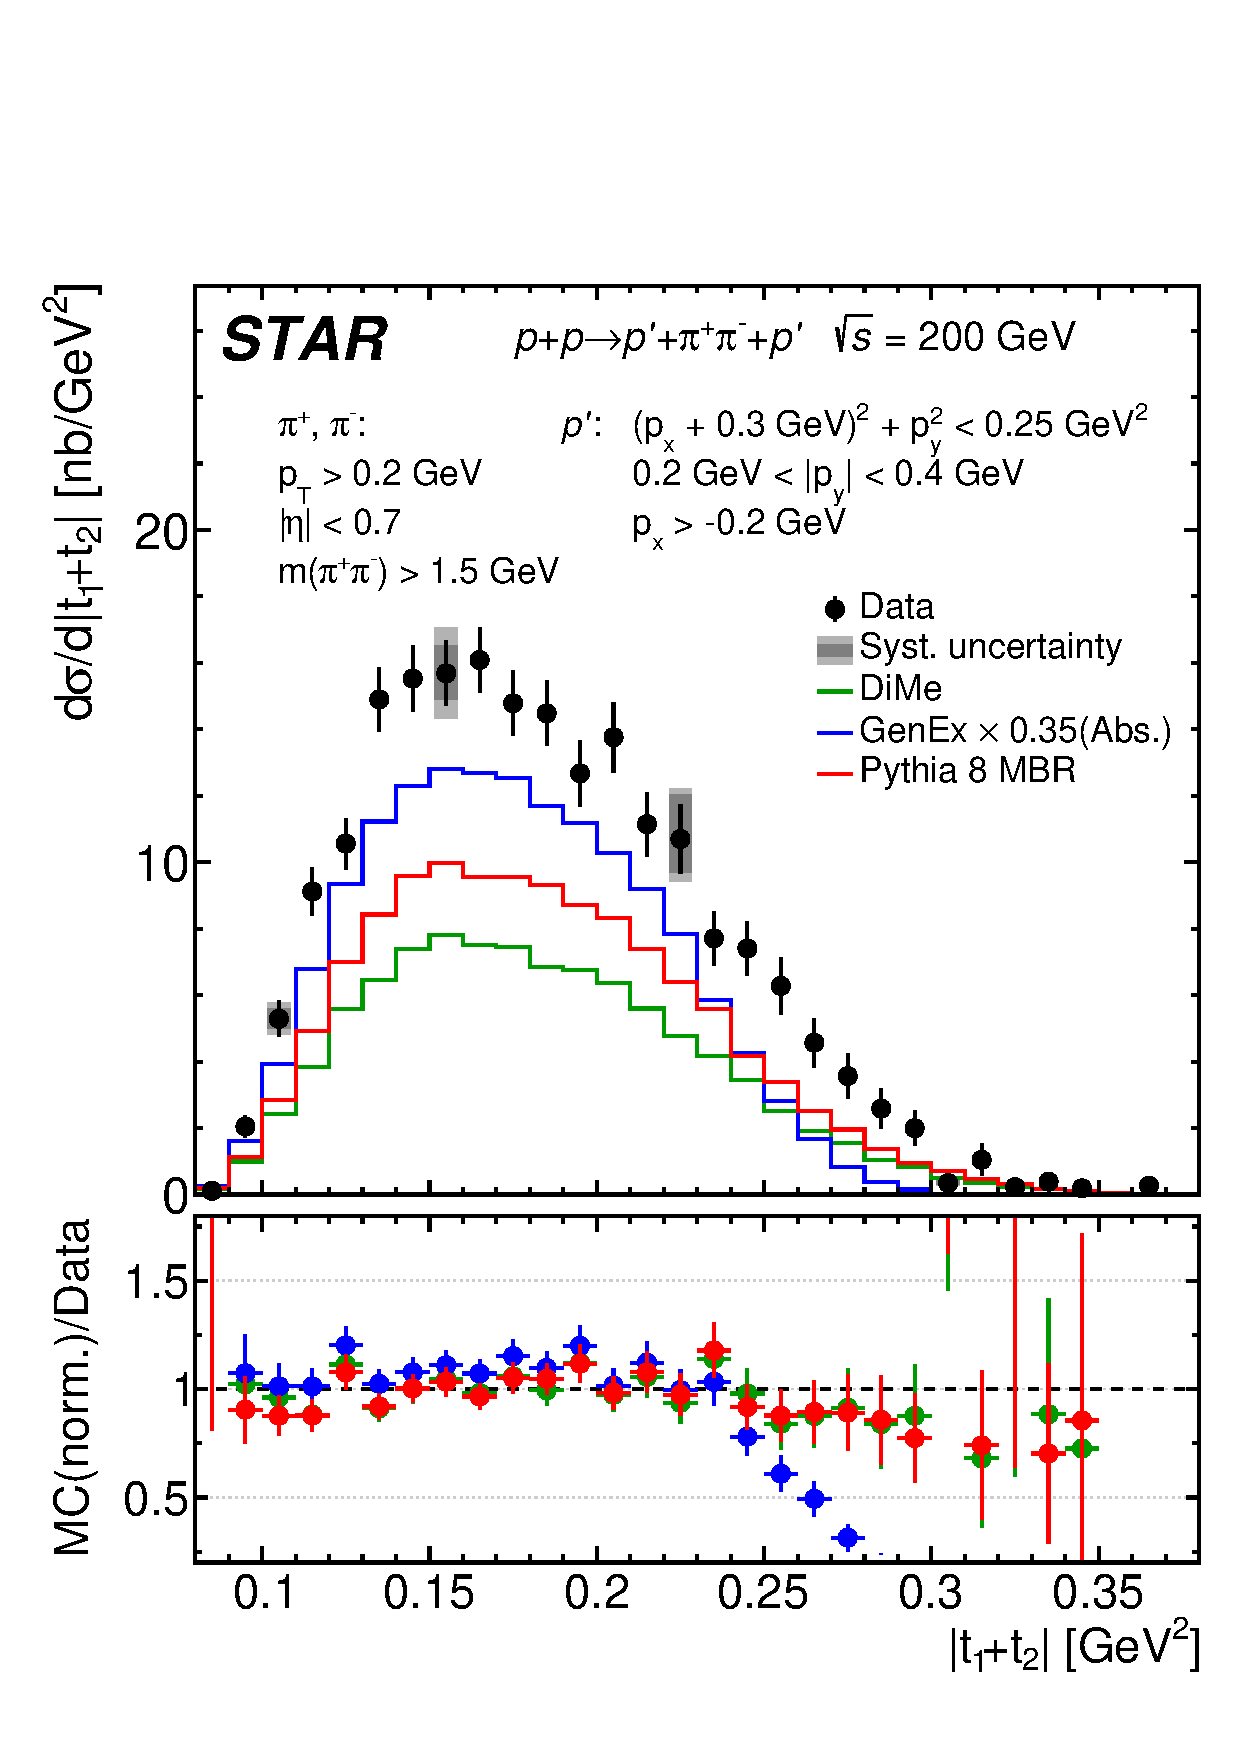
\includegraphics[width=.31\textwidth,page=1]{graphics/physicsResults/Ratio_FinalResult_MandelstamTSum_pion_MassBin_3.pdf}
%
\caption[Differential cross sections for CEP of $\pi^+\pi^-$ pairs as a function of the rapidity of the pair, difference of azimuthal angles of the forward scattered protons and of the sum of the squares of the four-momenta losses in the proton vertices measured in the fiducial region explained on the plots, separately for three ranges of the $\pi^+\pi^-$ pair invariant mass: $m<1$ GeV, $1<m<1.5$ GeV and $m>1.5$ GeV.]{Differential cross sections for CEP of $\pi^+\pi^-$ pairs as a function of the rapidity of the pair (left column) difference of azimuthal angles of the forward scattered protons (middle column) and of the sum of the squares of the four-momenta losses in the proton vertices (right column) measured in the fiducial region explained on the plots, separately for three ranges of the $\pi^+\pi^-$ pair invariant mass: $m<1$ GeV (top), $1<m<1.5$ GeV (middle) and $m>1.5$ GeV (bottom). Data are shown as solid points with error bars representing the statistical uncertainties. The typical systematic uncertainties are shown as gray boxes for only few data points as they are almost fully correlated between neighboring bins. Predictions from MC models GenEx, DiMe and MBR are shown as histograms. In the lower panels the ratios of the MC predictions scaled to data and the data are shown.}
\label{results_4}
\end{figure}
%
%\FloatBarrier
%
\begin{figure}[h]
\centering
\hspace*{5pt}
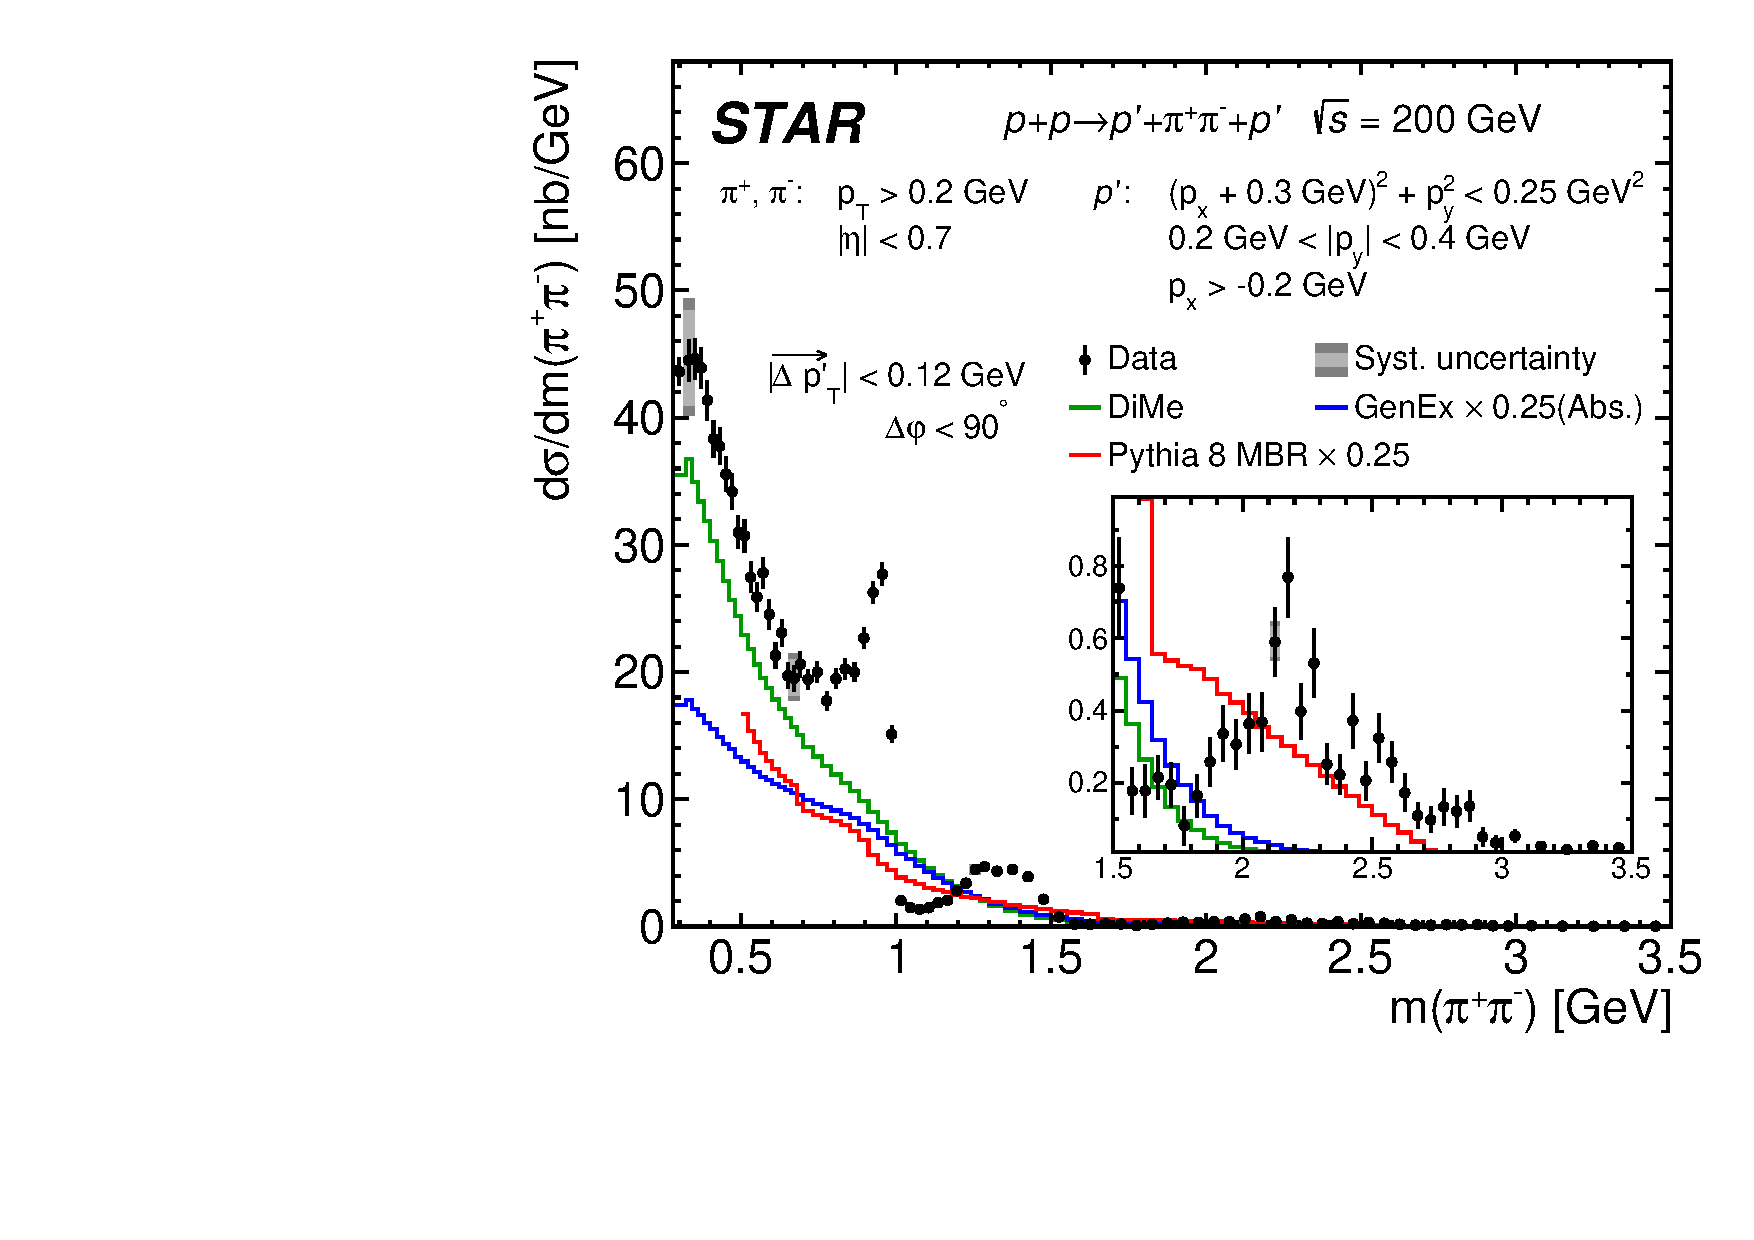
\includegraphics[width=.46\textwidth,page=1]{graphics/physicsResults/FinalResult_InvMass_pion_SmallDpt_DeltaPhiLessThan90.pdf}
\hfill
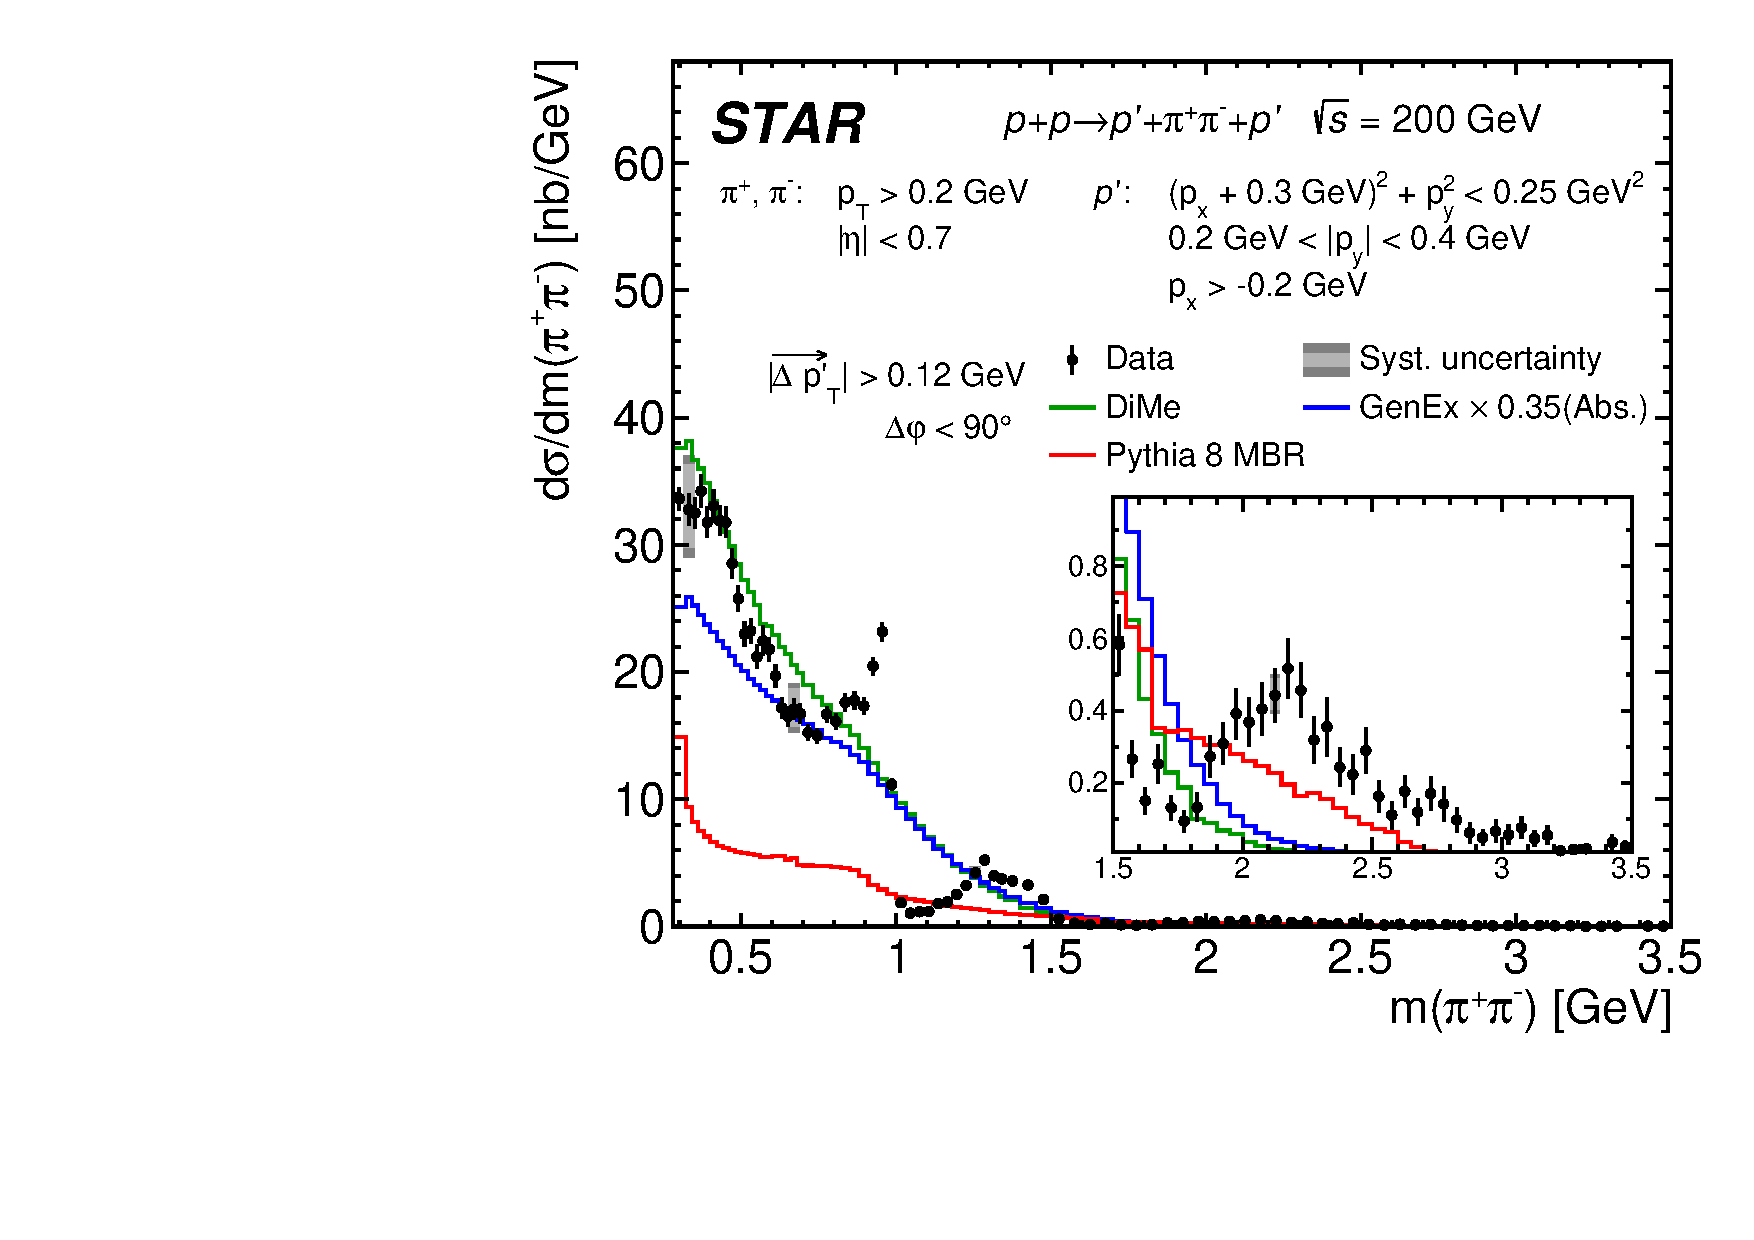
\includegraphics[width=.46\textwidth,page=1]{graphics/physicsResults/FinalResult_InvMass_pion_LargeDpt_DeltaPhiLessThan90.pdf}
\hspace*{5pt}
%
\caption[Differential cross sections $d\sigma/dm(\pi^+\pi^-)$ for CEP of $\pi^+\pi^-$ pairs in two $|\vec{p}_{1,T}^{\,\prime}-\vec{p}_{2,T}^{\,\prime}|$ regions: $|\vec{p}_{1,T}^{\,\prime}-\vec{p}_{2,T}^{\,\prime}|<0.12$ GeV and $|\vec{p}_{1,T}^{\,\prime}-\vec{p}_{2,T}^{\,\prime}|>0.12$ GeV in the fiducial region and $\Delta\phi<90$ degree.]{Differential cross sections $d\sigma/dm(\pi^+\pi^-)$ for CEP of $\pi^+\pi^-$ pairs in two $|\vec{p}_{1,T}^{\,\prime}-\vec{p}_{2,T}^{\,\prime}|$ regions: $|\vec{p}_{1,T}^{\,\prime}-\vec{p}_{2,T}^{\,\prime}|<0.12$ GeV (left) and $|\vec{p}_{1,T}^{\,\prime}-\vec{p}_{2,T}^{\,\prime}|>0.12$ GeV (right)  in the fiducial region and $\Delta\phi<90$ degree. There is no difference for two $|\vec{p}_{1,T}^{\,\prime}-\vec{p}_{2,T}^{\,\prime}|$ regions. Data are shown as solid points with error bars representing the statistical uncertainties. The typical systematic uncertainties are shown as gray boxes for only few data points as they are almost fully correlated between neighboring bins. Predictions from MC models GenEx, DiMe and MBR are shown as histograms.}
\label{results_5}
\end{figure}


% We have also studied angular distributions of the charged particles produced in the final state. This can be done in various reference frames. However, for an easy comparison with theoretical predictions we use here the Collins-Soper \cite{cs_frame} reference frame also used e.g. in Ref.~\cite{lebiedowicz_3}. Collins-Soper frame is the centre-of-mass frame of the charged particles pair with the $z$-axis making equal angles with the beam protons momenta which in addition define the new $x-z$ plane. It can be reached from the laboratory frame (proton-proton c.m.s.) in two steps. First, boost along the $z$-axis to an intermediate frame in which the pair longitudinal momentum is equal to zero. In this frame the beam protons momenta remain parallel to the $z$-axis and the transverse momentum of the pair remains unchanged. Second, boost in the direction of the transverse momentum of the pair, to get to the pair c.m.s. frame.
%
\begin{figure}[h]
\centering
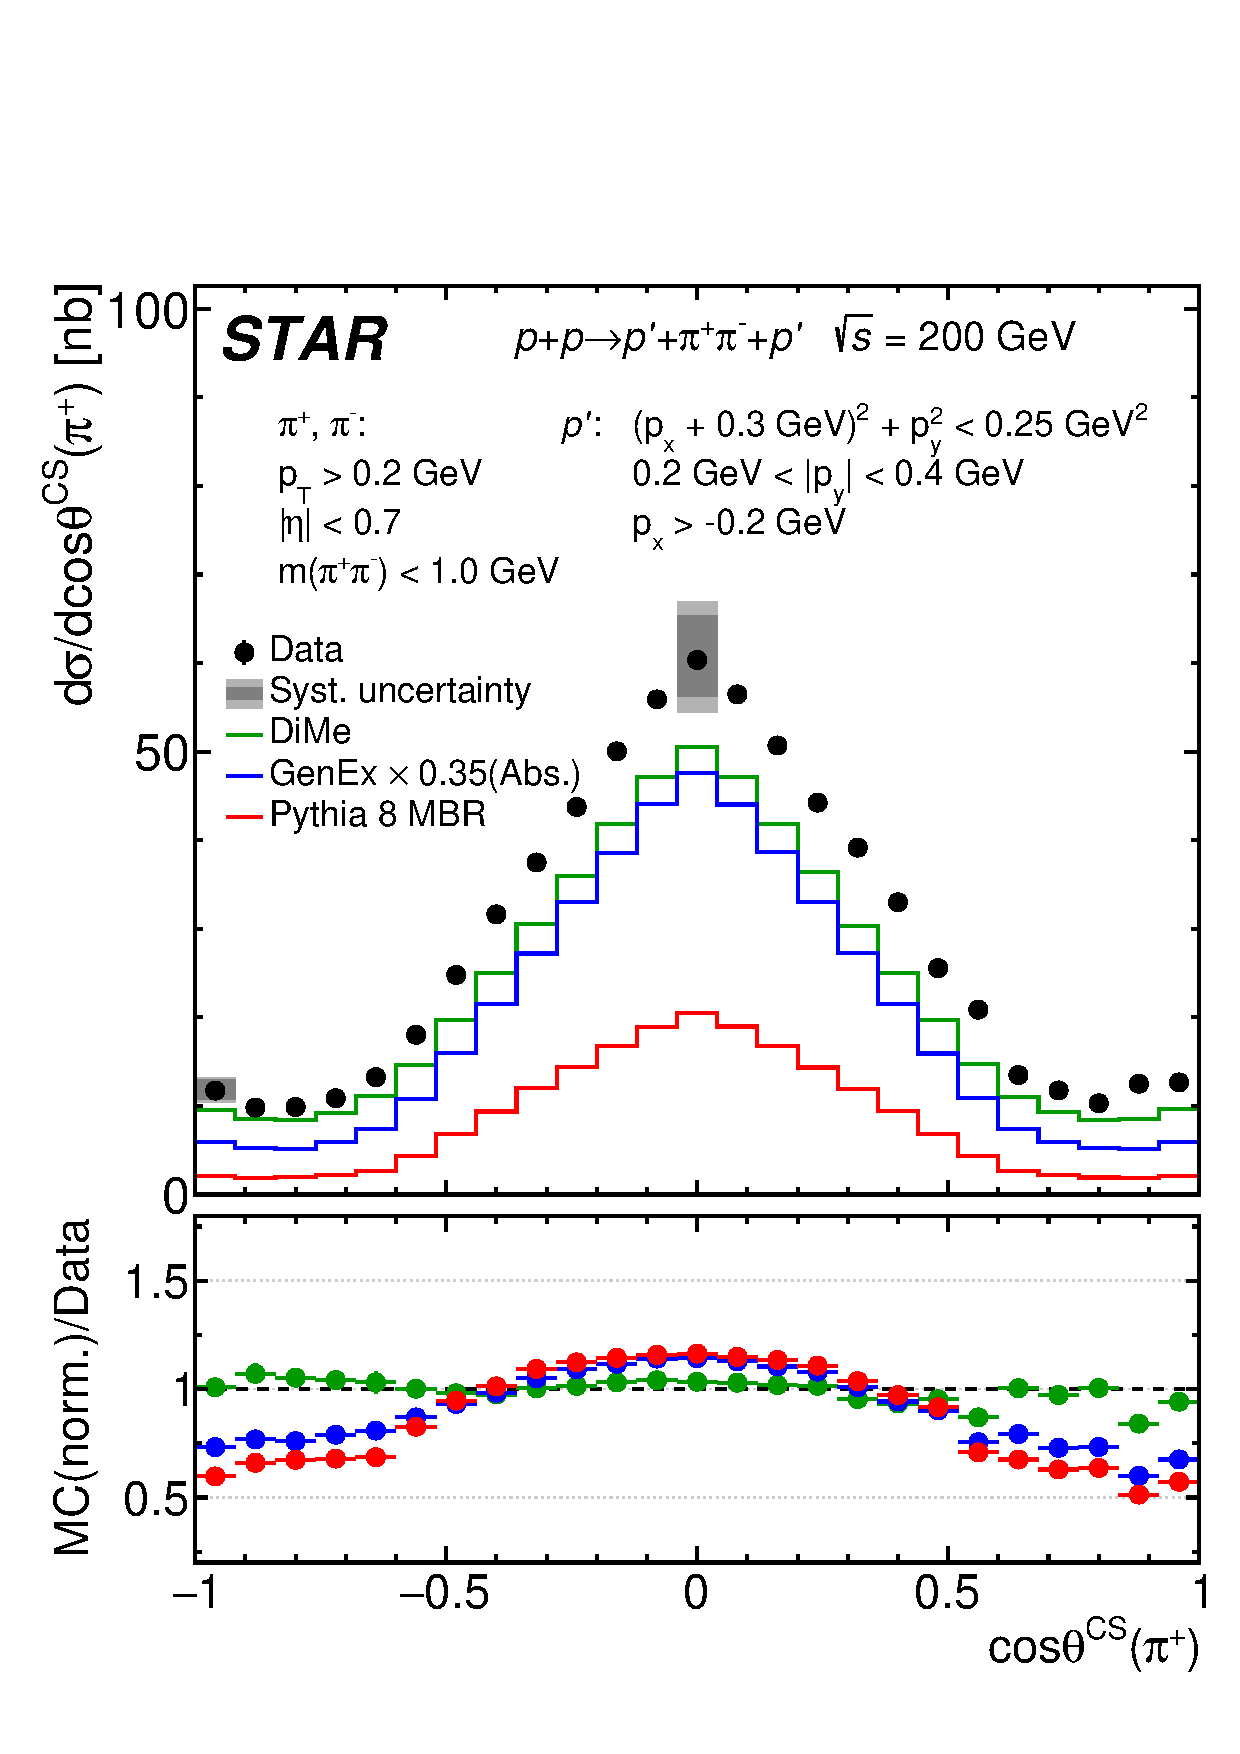
\includegraphics[width=.31\textwidth,page=1]{graphics/physicsResults/Ratio_FinalResult_CosThetaCS_pion_MassBin_1.pdf}
\hfill
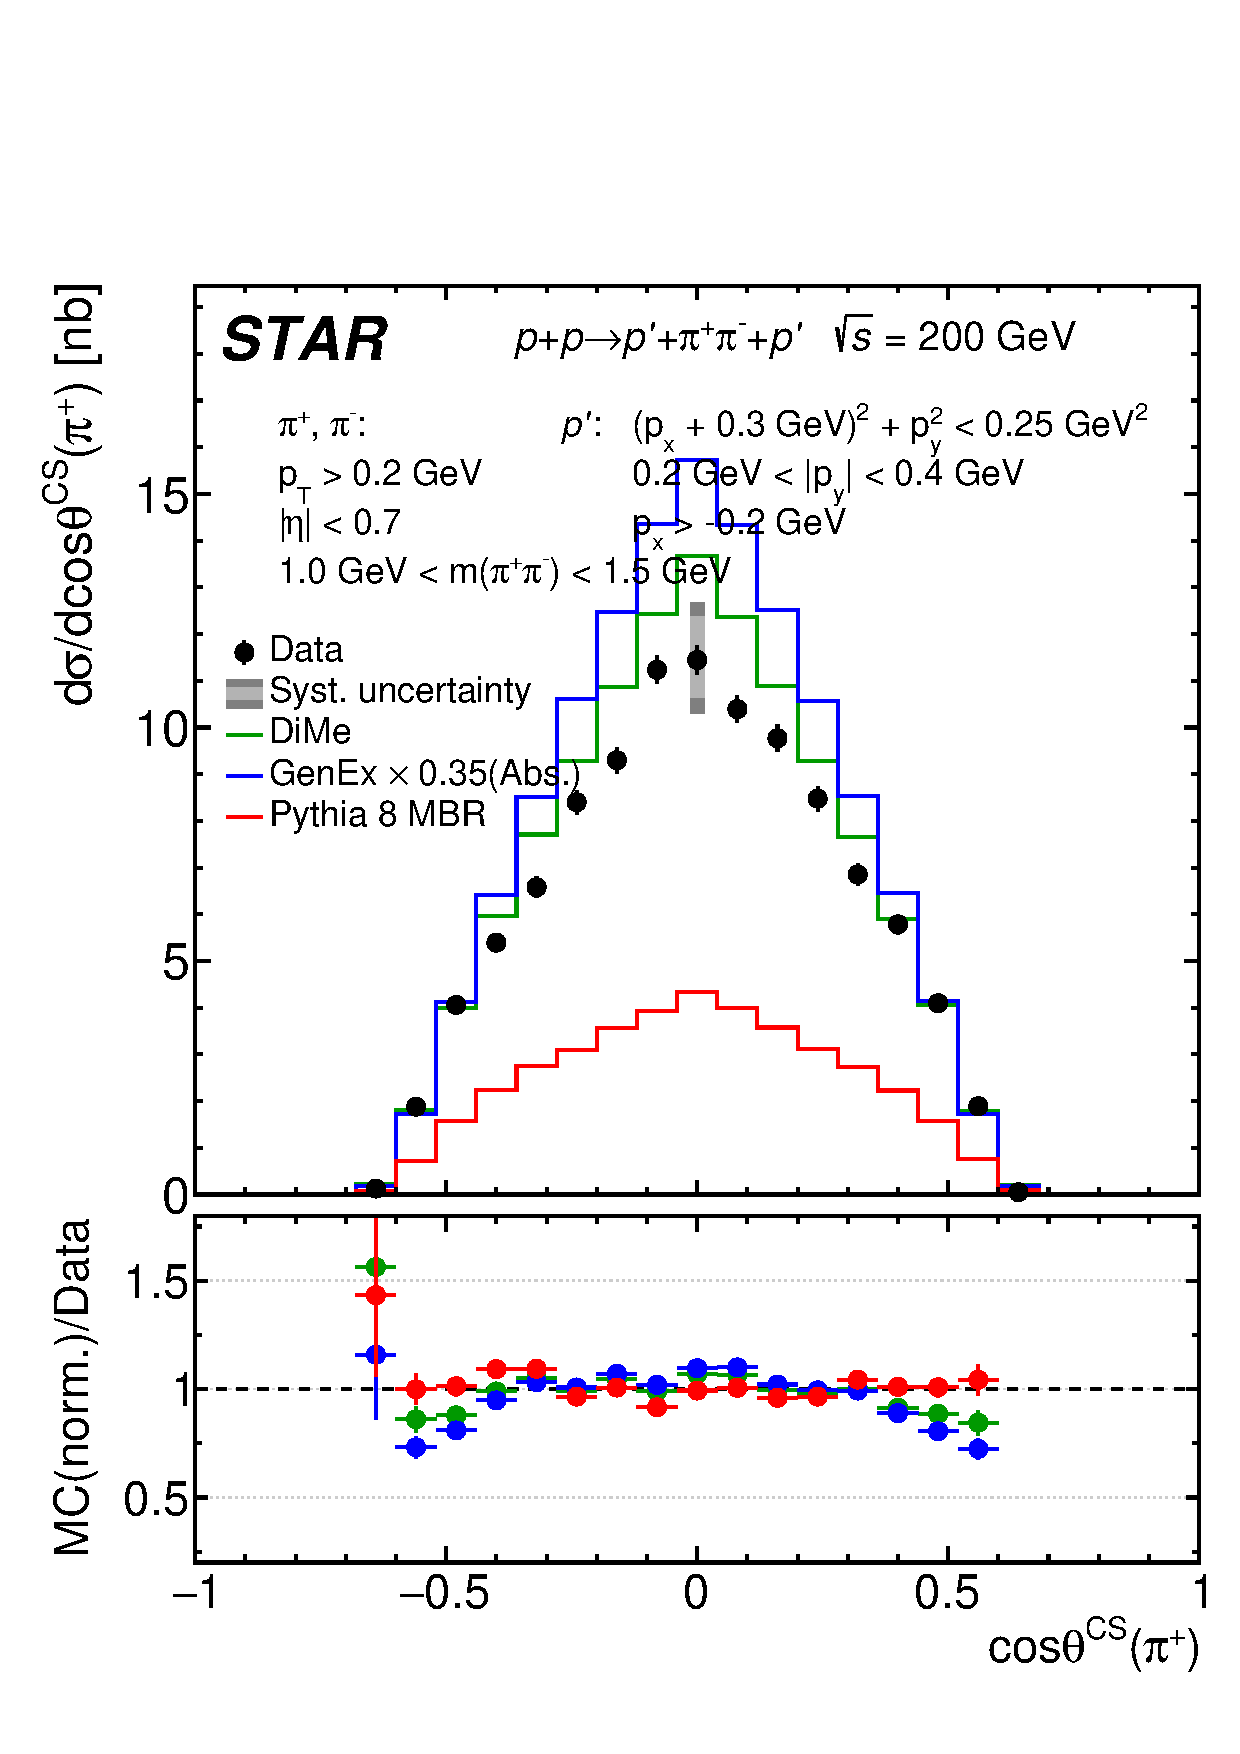
\includegraphics[width=.31\textwidth,page=1]{graphics/physicsResults/Ratio_FinalResult_CosThetaCS_pion_MassBin_2.pdf}
\hfill
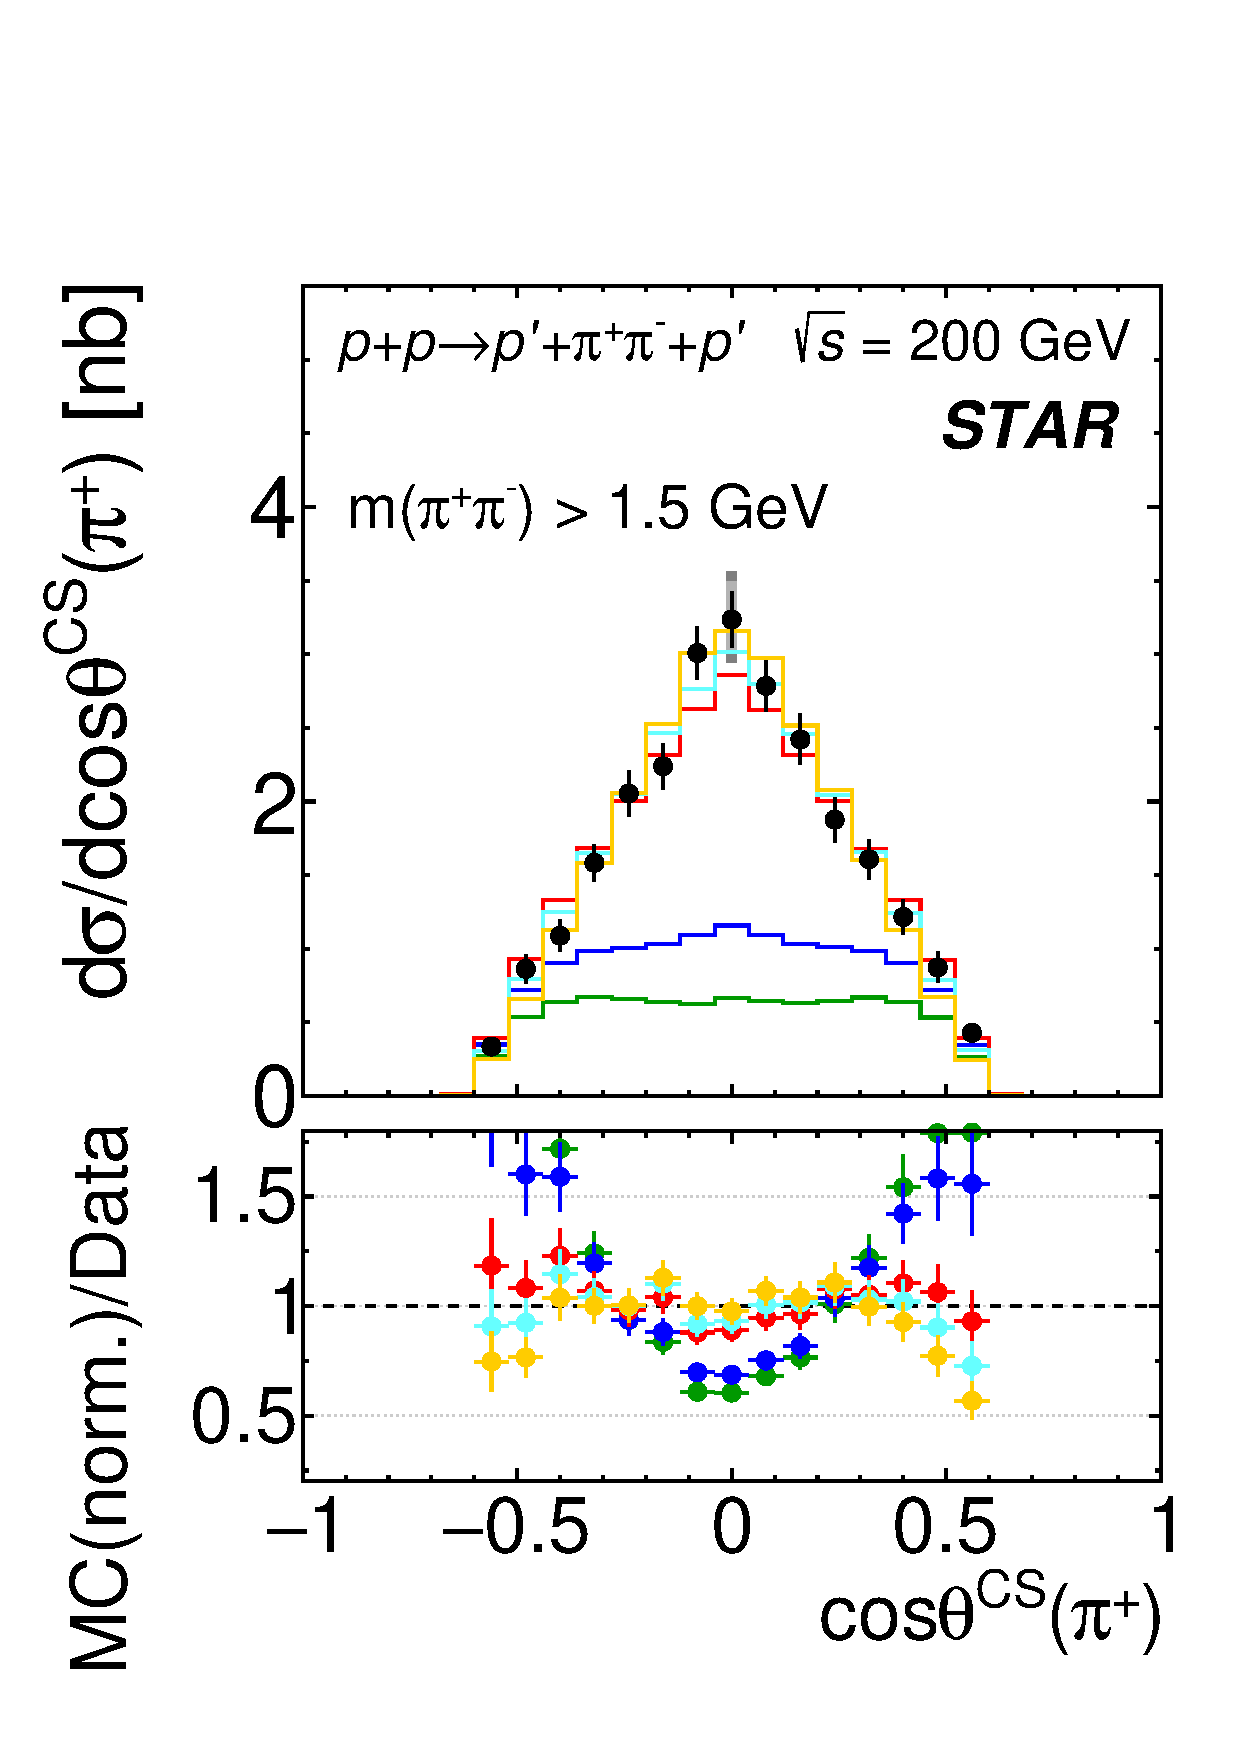
\includegraphics[width=.31\textwidth,page=1]{graphics/physicsResults/Ratio_FinalResult_CosThetaCS_pion_MassBin_3.pdf}
\newline
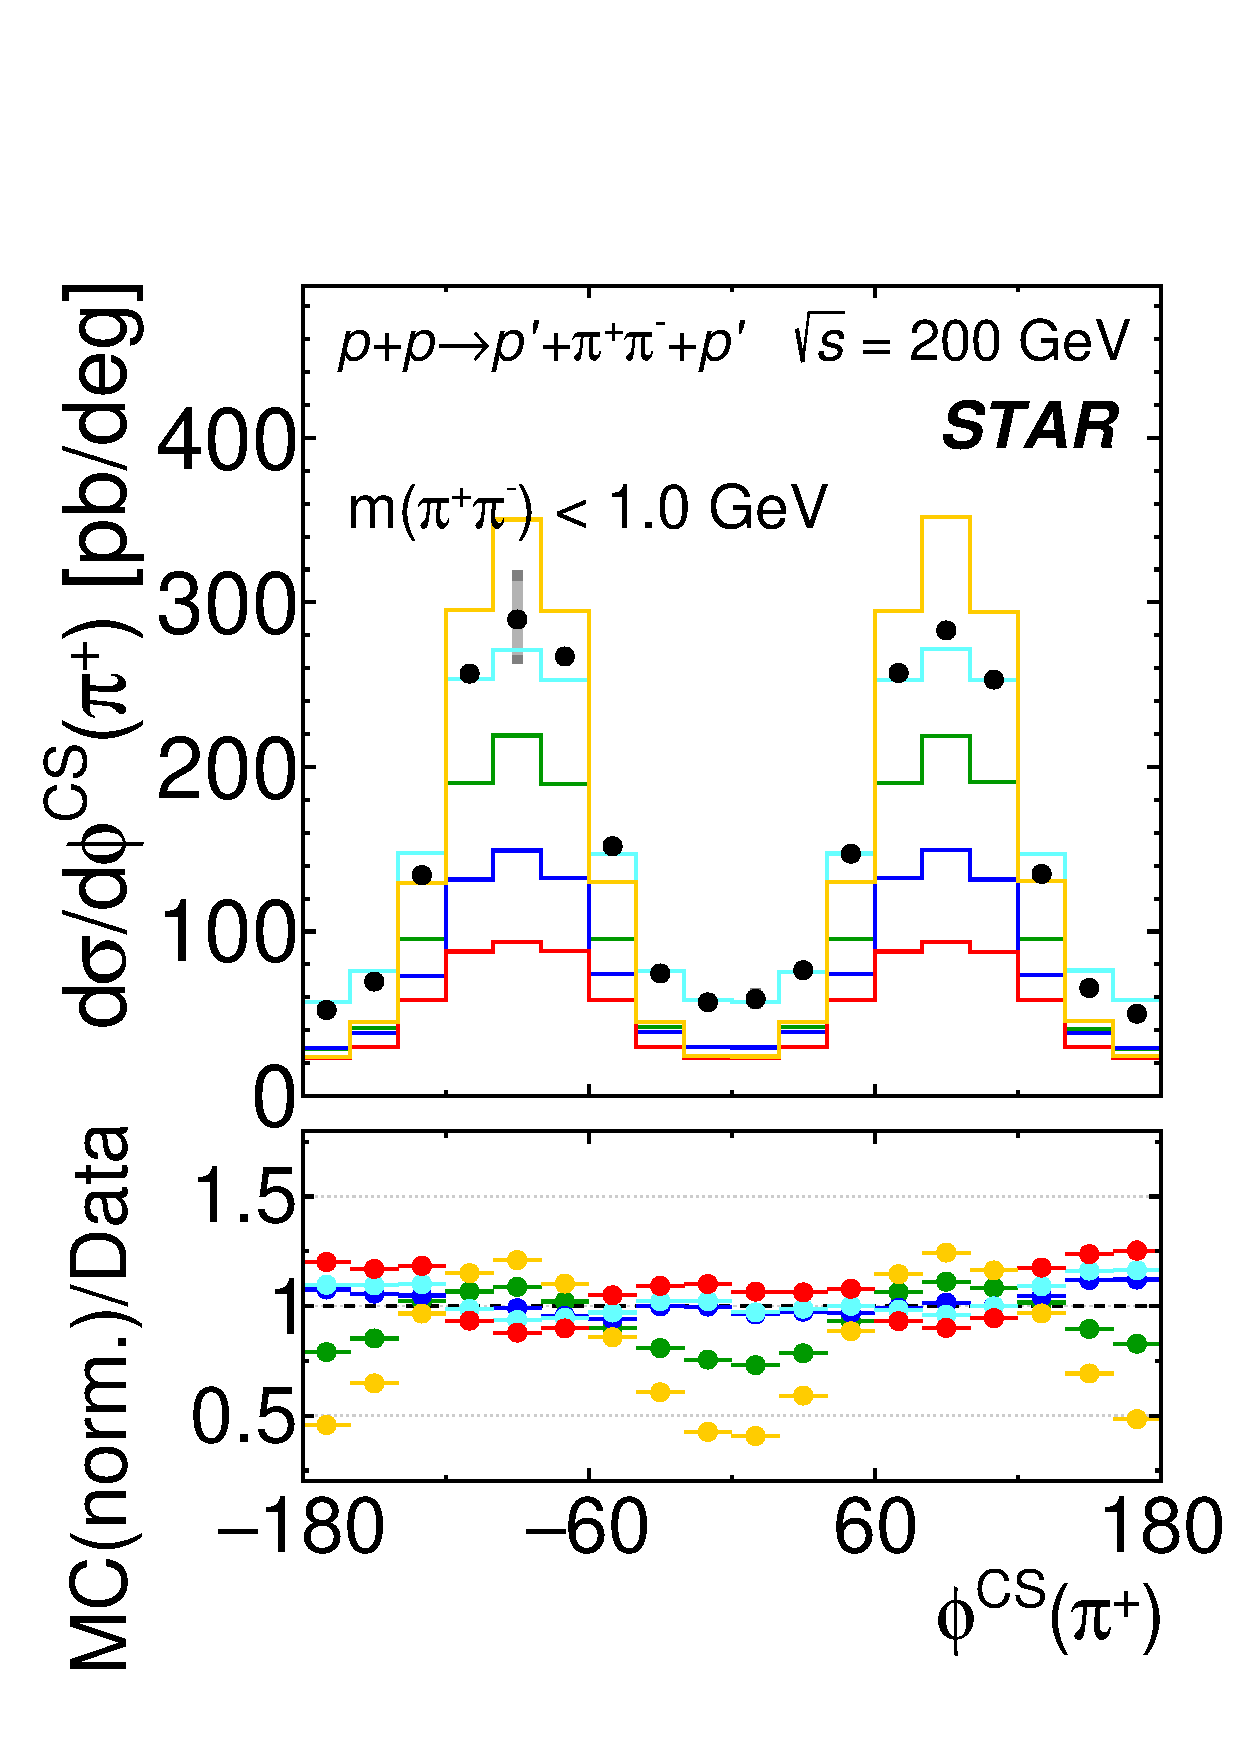
\includegraphics[width=.31\textwidth,page=1]{graphics/physicsResults/Ratio_FinalResult_PhiCS_pion_MassBin_1.pdf}
\hfill
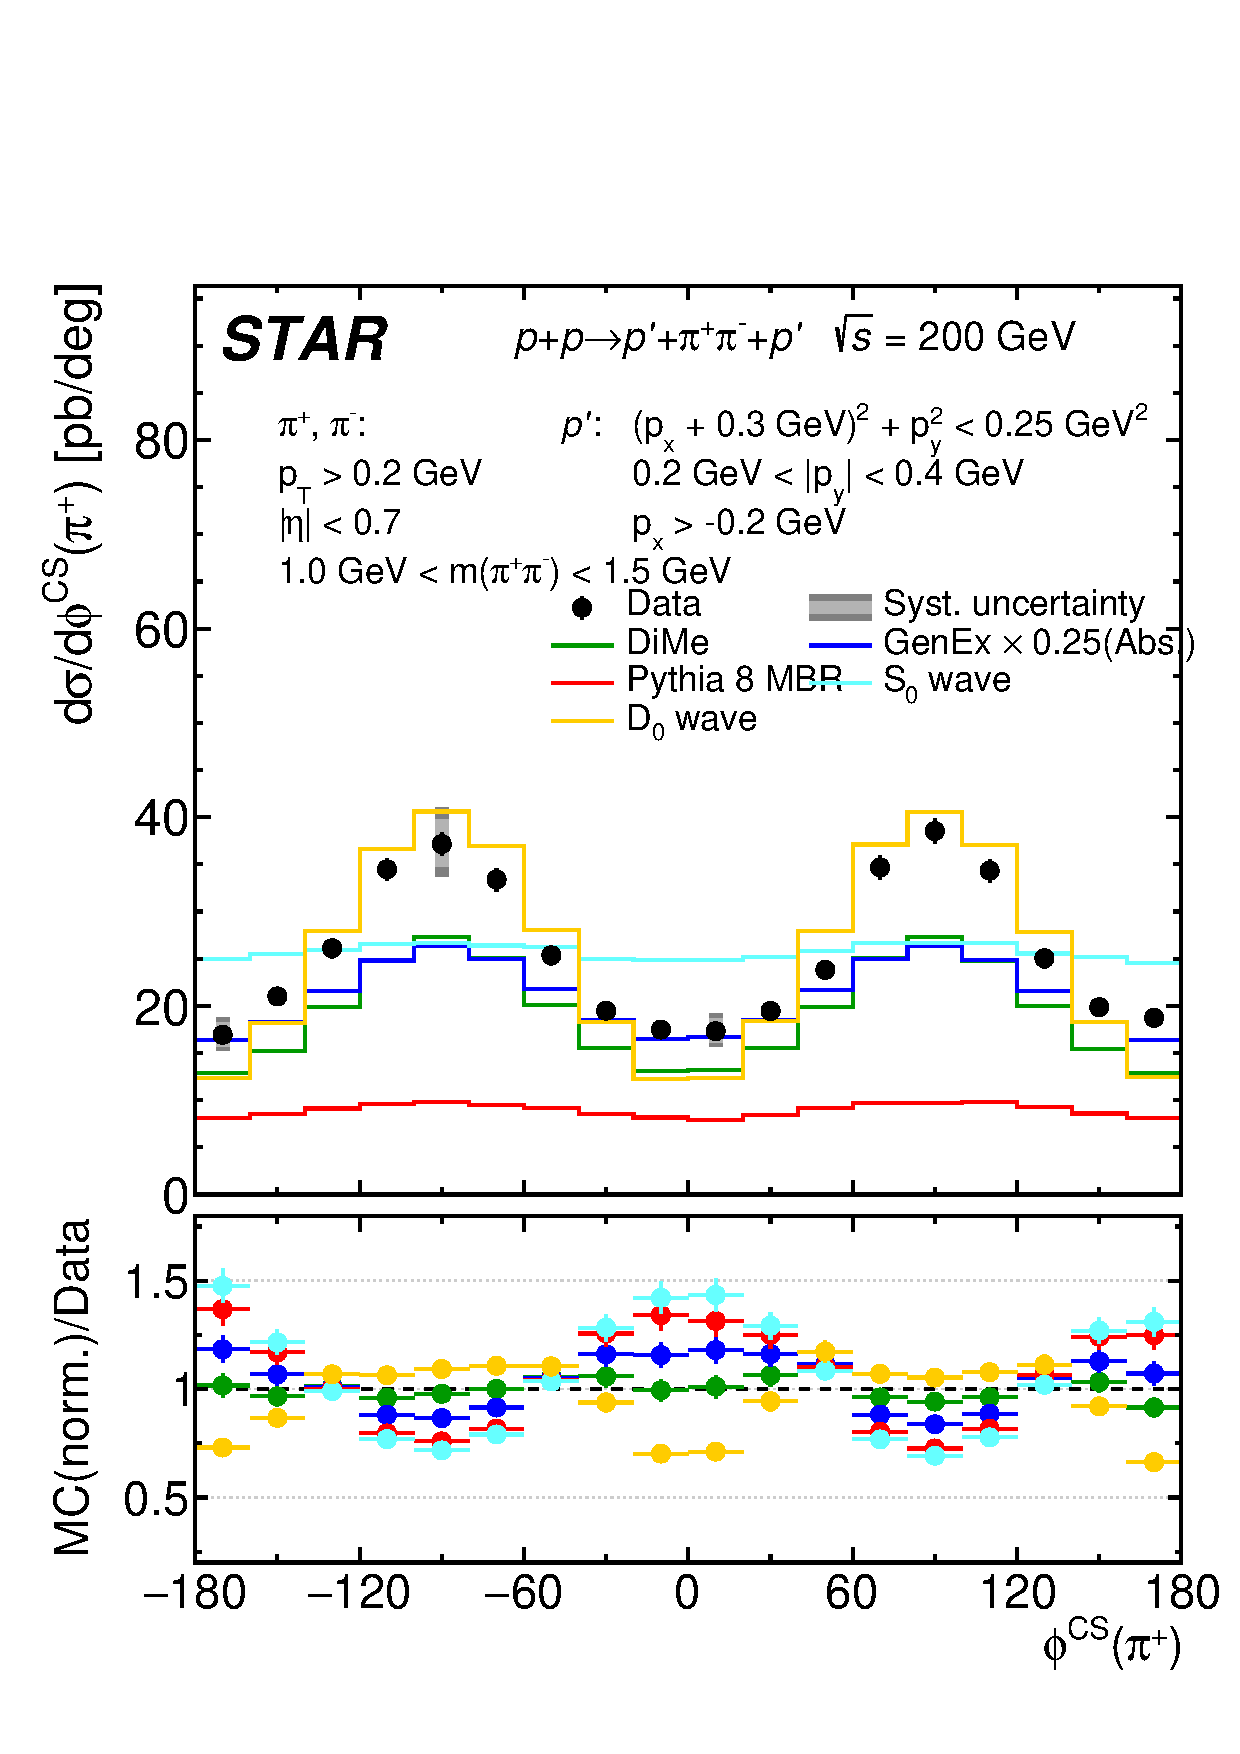
\includegraphics[width=.31\textwidth,page=1]{graphics/physicsResults/Ratio_FinalResult_PhiCS_pion_MassBin_2.pdf}
\hfill
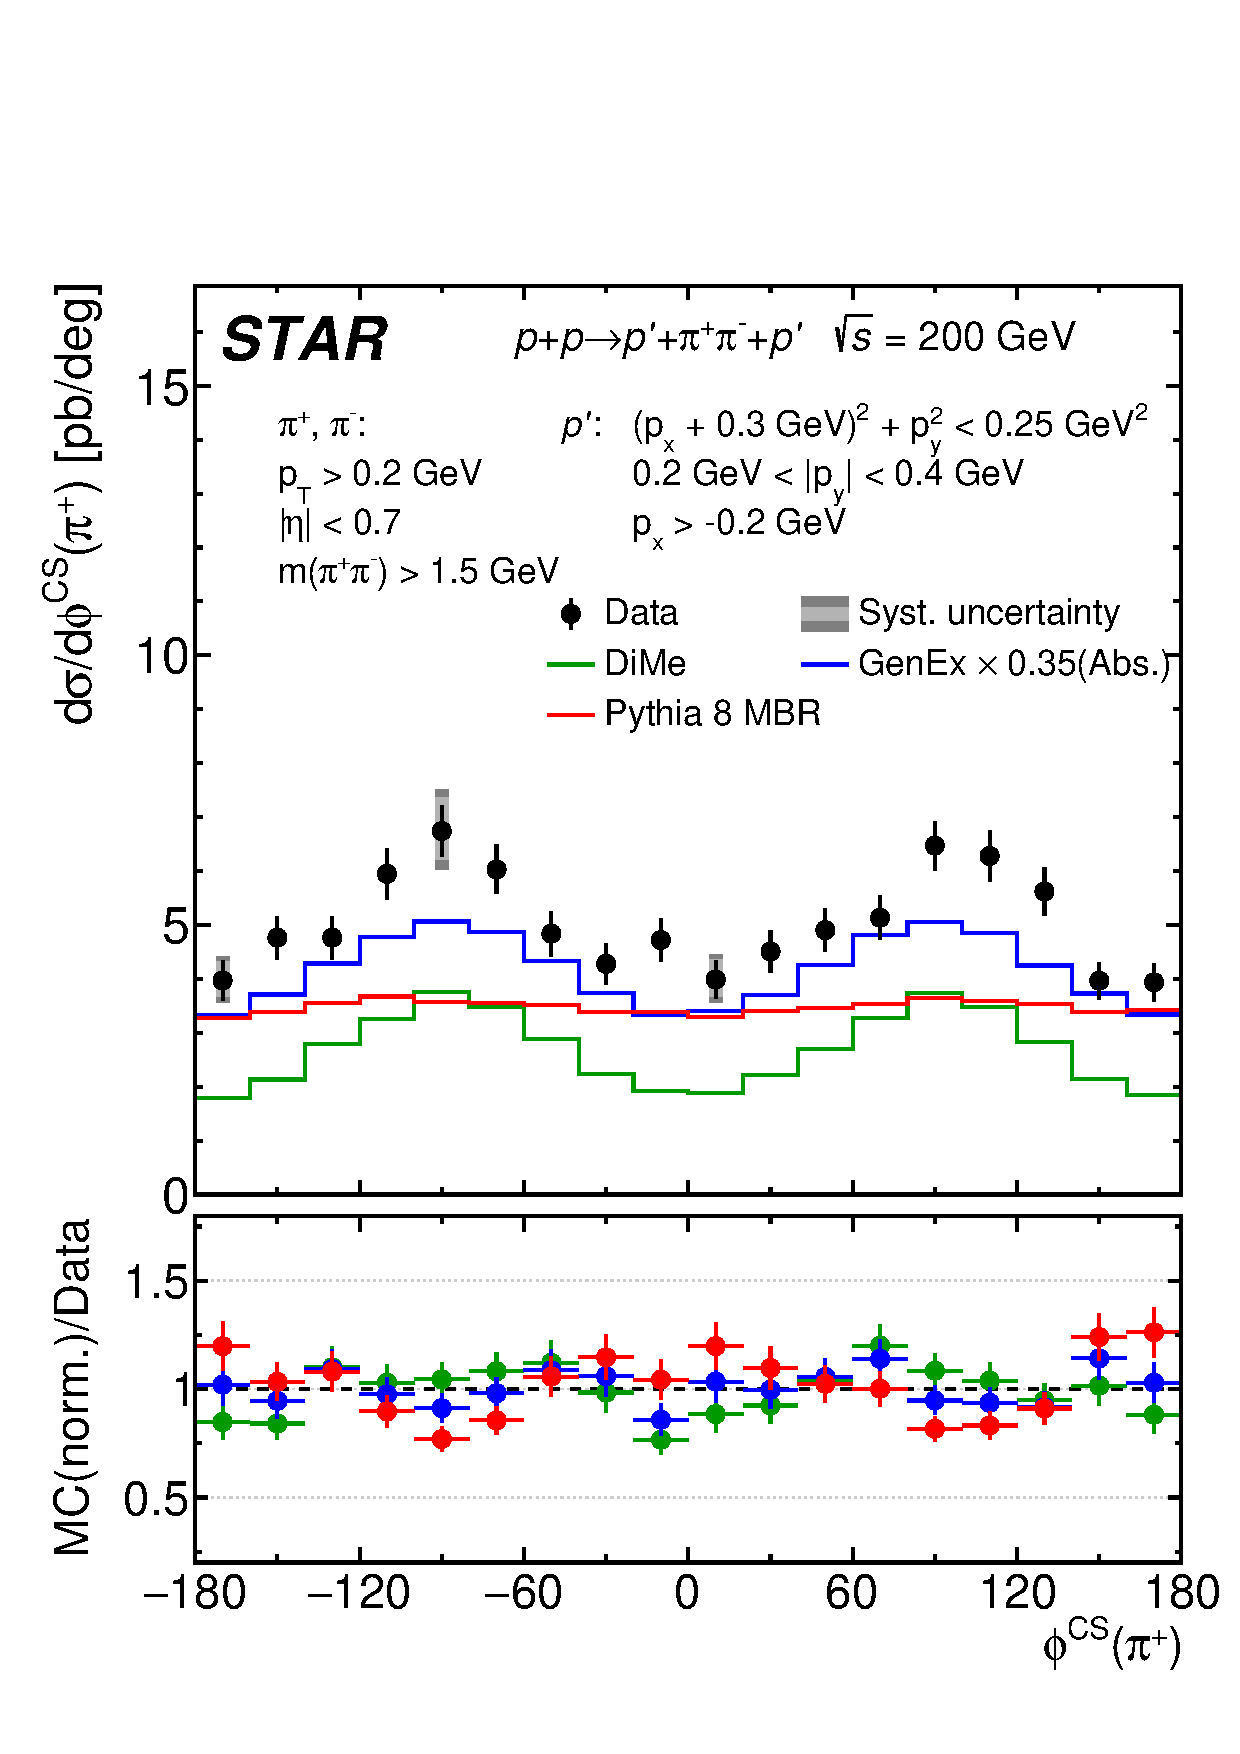
\includegraphics[width=.31\textwidth,page=1]{graphics/physicsResults/Ratio_FinalResult_PhiCS_pion_MassBin_3.pdf}
%
\caption[Differential cross sections for CEP of $\pi^+\pi^-$ pairs as a function of $\cos{\theta^\mathrm{CS}}$ and of $\phi^\mathrm{CS}$ measured in the fiducial region explained on the plots, separately for three ranges of the $\pi^+\pi^-$ pair invariant mass: $m<1$ GeV, $1<m<1.5$ GeV and $m>1.5$ GeV.]{Differential cross sections for CEP of $\pi^+\pi^-$ pairs as a function of $\cos{\theta^\mathrm{CS}}$ (top) and of $\phi^\mathrm{CS}$ (bottom)  measured in the fiducial region explained on the plots, separately for three ranges of the $\pi^+\pi^-$ pair invariant mass: $m<1$ GeV (left column), $1<m<1.5$ GeV (middle column) and $m>1.5$ GeV (right column). Data are shown as solid points with error bars representing the statistical uncertainties. The typical systematic uncertainties are shown as gray boxes for only few data points as they are almost fully correlated between neighboring bins. Predictions from MC models GenEx, DiMe and MBR are shown as histograms. In the lower panels the ratios of the MC predictions scaled to data and the data are shown.}
\label{results_7}
\end{figure}


\section{Invariant mass spectrum modelling}\label{sec:InvMassFit}

We make an attempt to fit extrapolated (using acceptance corrections from Sec.~\ref{sec:geomCorr}) differential cross-section with a simplified model of the $\pi^{+}\pi^{-}$ invariant mass spectrum. In this model we assume contributions from the direct pair production and three resonances in the mass range of $0.6-1.7$ GeV: $f_0(980)$, $f_2(1270)$ and $f_0(1500)$. It is important to note, that in the fit only $f_{2}(1270)$ has fixed mass and width and thus is explicitly assumed. For the other two resonances the masses and widths are left free, however their fitted masses and widths are compatible with $f_0(980)$ and $f_0(1500)$, therefore we use such labeling from the very beginning.

The total amplitude for the exclusive $\pi^{+}\pi^{-}$ production is given by:
% 
\begin{equation}
\label{eq:amplitude}
\begin{aligned}
A(m) = & \;A_{\textrm{cont}}\times f_{\textrm{cont}(m)}+ \\
        & \;A_{\textrm{f}_0(980)} \times \mathcal{R}_{\textrm{F}}\left(m;M_{f_0(980)},\Gamma_{f_0(980)}\right)+ \\
        & \;A_{\textrm{f}_2(1270)} \times \mathcal{R}_{\textrm{BW}}\left(m;M_{f_2(1270)},\Gamma_{f_2(1270)}\right) +\\
        & \;A_{\textrm{f}_0(1500)} \times \mathcal{R}_{\textrm{BW}}\left(m;M_{f_0(1500)},\Gamma_{f_0(1500)}\right),\\
\end{aligned}
\end{equation}
%
thus all states are added coherently (interfere with each other). The amplitude for continuum production is chosen to be real while multiplicative amplitude factors for resonances are allowed to be complex:
\begin{equation}A_{\textrm{cont}}\in\mathbb{R},~~~A_{\textrm{f}_0(980)},A_{\textrm{f}_2(1270)},A_{\textrm{f}_0(1500)}\in\mathbb{C}~~~~\rightarrow~~~~A_{\textrm{f}}=|A_{\textrm{f}}|e^{i\phi_{\textrm{f}}}.\end{equation}
%
The shape of the continuum amplitude is assumed to have the form
\begin{equation}f_{\textrm{cont}}(m) = \sqrt{\frac{q}{m}}\times e^{-\frac{B}{2}\cdot q}\end{equation}
with the break-up momentum $q$ equal to
\begin{equation}\label{eq:breakupMom}
q(m) = \frac{1}{2}\sqrt{m^{2}-4m_{\pi}^{2}}.
\end{equation}
For $f_2(1270)$ and $f_0(1500)$ resonances we use relativistic Breit-Wigner form of the production amplitude with mass-dependent width:
\begin{equation}\label{eq:BW}\mathcal{R}_{\textrm{BW}}(m;M,\Gamma_{0}) = \frac{M\sqrt{\Gamma_{0}}\sqrt{\Gamma(m)}}{M^{2}-m^{2}-i M\Gamma(m)},~~\Gamma(m) = \Gamma_{0}\frac{q}{m}\frac{M}{q_{0}}\left(\frac{B_{J}(q^{2}R^{2})}{B_{J}(q_{0}^{2}R^{2})}\right)^{2}.\end{equation}
The centrifugal effects in Eq.~\eqref{eq:BW} are accounted through the Blatt-Weisskopf barrier factors $B_{J}$~\cite{BarrierFactors} with the empirical interaction radius $R$ set to 1~fm and $q_{0} = q(M)$. Naturally $J=2$ and $J=0$ is used for $f_2(1270)$ and $f_0(1500)$, respectively.

Meson $f_0(980)$ requires different treatment due to large branching ratio to $K\bar{K}$ channel which opens in the vicinity of the mass peak. This changes the resonance shape and is accounted for in the parametrisation of the amplitude via the Flatt\'e formula~\cite{Flatte}:
\begin{equation}\label{eq:Flatte}\mathcal{R}_{\textrm{F}}(m;M,\Gamma_{0}) = \frac{M\sqrt{\Gamma_{0}}\sqrt{\Gamma_{\pi}(m)}}{M^{2}-m^{2}-i M\left(\Gamma_{\pi}(m)+\Gamma_{K}(m)\right)}\end{equation}
%
with the partial width $\Gamma_{j}$ ($j=\pi, K$) described by the product of the coupling parameter $g_{j}$ and the break-up momentum $q$ (Eq.~\eqref{eq:breakupMom}) for particle $j$:
\begin{equation}
    \Gamma_{j}(m) = g_{j}q_{j}(m) = \frac{g_{j}}{2}\sqrt{m^{2}-4m_{j}^{2}}.
\end{equation} and the partial width in $\pi^{+}\pi^{-}$ channel at the resonance mass equal to
\begin{equation}
    \Gamma_{0} = g_{\pi}q_{\pi}(M).
\end{equation}
In the fit the ratio $g_{K}/g_{\pi}$ is fixed to 4.21, the value well constrained experimentally through the measurement of $J/\psi$ decay into $\phi$ and $\pi^{+}\pi^{-}$/$K^{+}K^{-}$~\cite{BES_JPsi}.
%

Squared amplitude from Eq.~\eqref{eq:amplitude}, $|A|^{2}$, is convoluted for the purpose of the fit with the normal distribution $\mathcal{N}(m; \sigma_{\text{res}})$ representing finite resolution of reconstructed invariant mass of the pion pair. The resolution parameter $\sigma_{\text{res}}$ is provided to the fitting algorithm; it is set to grow linearly with increasing invariant mass according to MC simulation of the STAR TPC detector. The $m(\pi^{+}\pi^{-})$ resolution at the lower and upper limit of the fit range is equal to 4~MeV and 13~MeV, respectively. The final form of function fitted to extrapolated $d\sigma/dm(\pi^{+}\pi^{-})$ is given by
\begin{equation}
    \mathcal{F}(m) = \int\limits_{m-3.5\cdot\sigma_{\text{res}}(m)}^{m+3.5\cdot\sigma_{\text{res}}(m)}dm'\mathcal{N}\left(m'-m; \sigma_{\text{res}}(m')\right)|A(m')|^{2}.
\end{equation}

The fitting is performed using Minuit2 toolkit~\cite{Minuit2} within the ROOT analysis software~\cite{ROOT}. The standard-defined $\chi^{2}$ is minimized simultaneously in two $\Delta\varphi$ ranges with the masses and widths of both $f_0$'s forced to be equal, while phases and absolute values of $f_2$ and $f_0$'s amplitudes left independent in the two $\Delta\varphi$ subsets. The mass and width of $f_2(1270)$ resonance is fixed to the well known Particle Data Group values~\cite{pdg}.
%
Experimental systematic uncertainties of the model parameters are estimated through the independent fits to extrapolated $d\sigma/dm(\pi^{+}\pi^{-})$ (Appendix~\ref{appendix:invMassSystFits}) with applied each of the systematic variations described in Sec.~\ref{sec:systEffectsList}. In addition to this we take into consideration sensitivity of the fit result related to the modelling of extrapolation to full kinematic region. We check the effect of extrapolation to full solid angle in $\pi^{+}\pi^{-}$ rest frame assuming smooth transition from the angular distributions for pure $S_{0}$ wave up to 1~GeV, to the angular distributions for pure $D_{0}$-wave starting from 1.2~GeV. We also check the effect of using extrapolation calculated with predictions from DiMe and GenEx generators, for both the central state and for the forward scattered protons. Also, we check the result of the fit with the ratio $g_{K}/g_{\pi}$ varied within its uncertainties.
At the end, systematic uncertainty on a parameter is calculated as a quadratic sum of the differences between the nominal fit result and the result of the fit to $d\sigma/dm(\pi^{+}\pi^{-})$ with each systematic effect considered except differences related to the extrapolation which are separated from experimental uncertainties and quoted as the largest deviation from nominal result.

\begin{figure}%[t] 
\centering
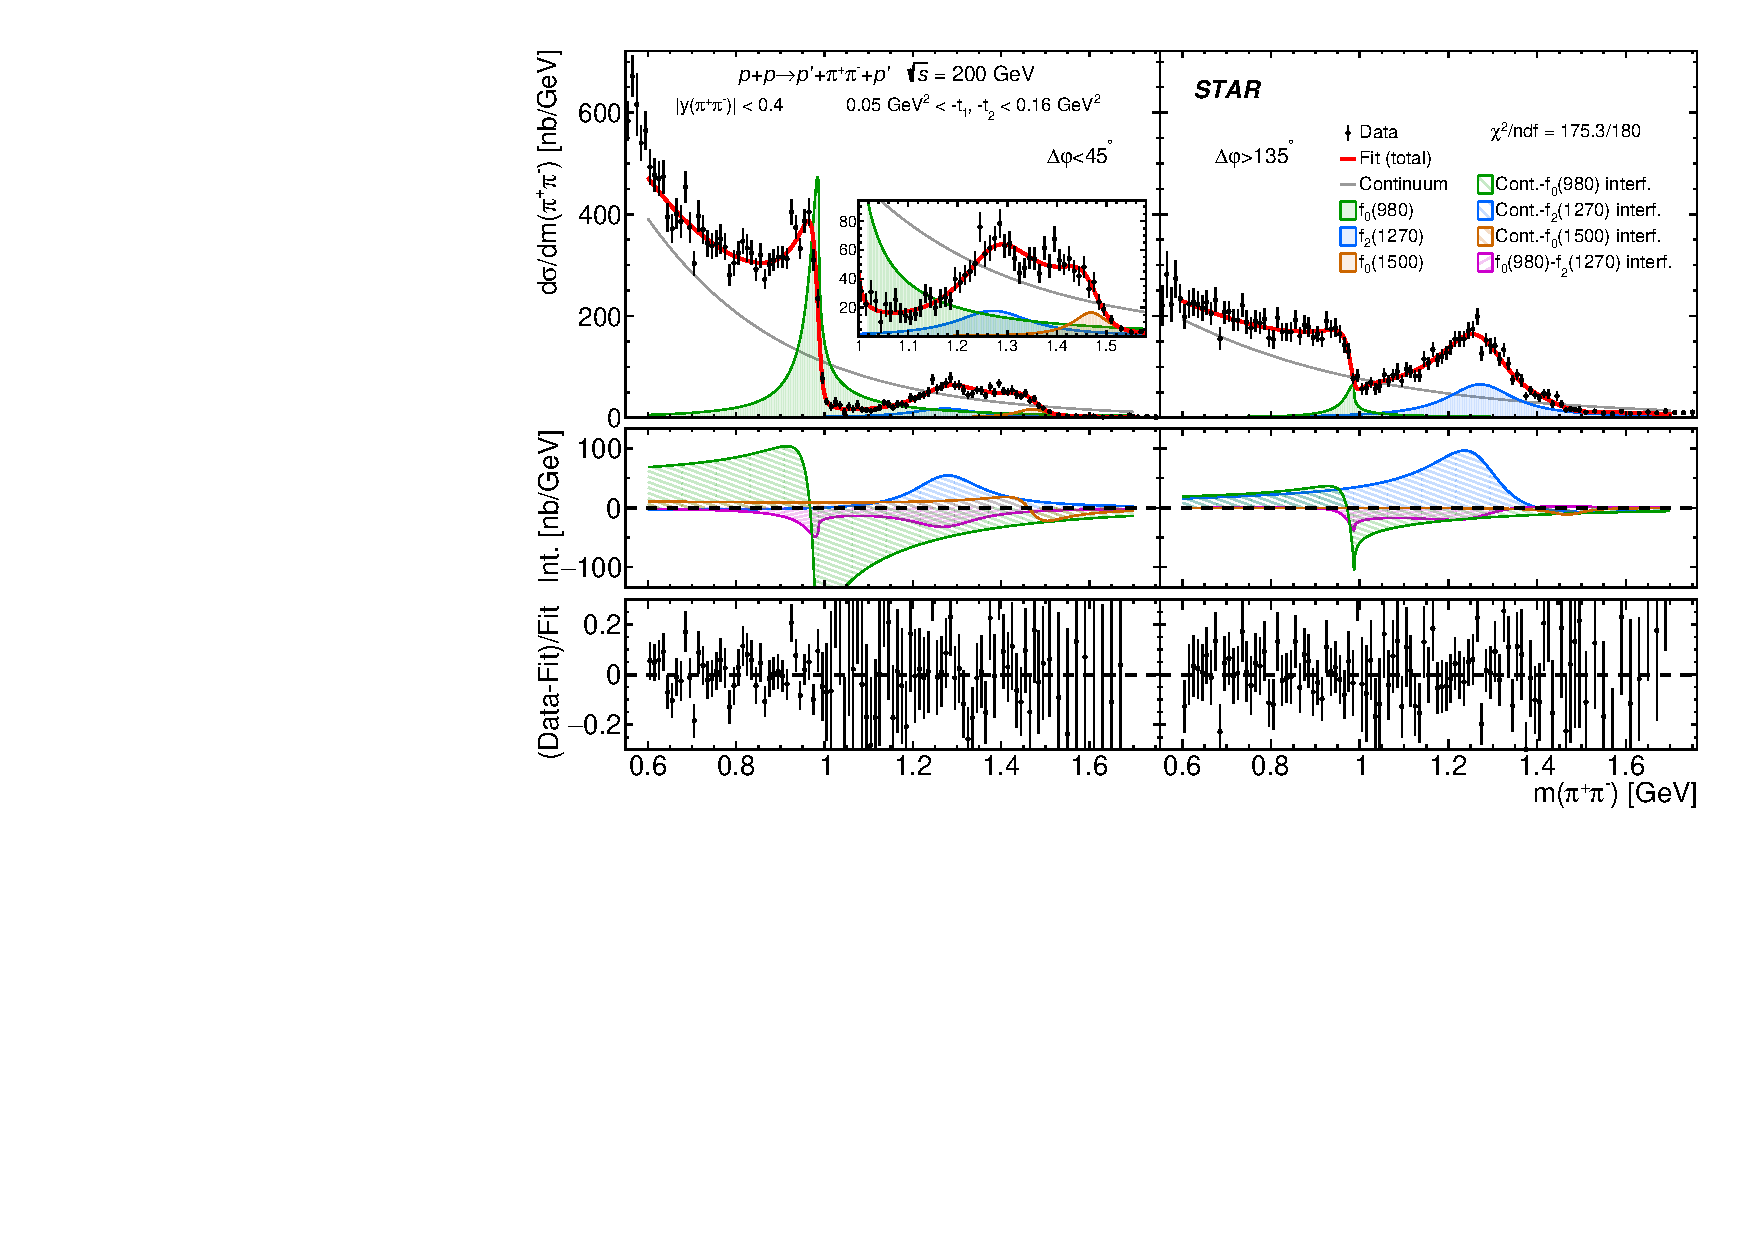
\includegraphics[width=\textwidth,page=1]{graphics/physicsResults/InvMassFit/RatioAndInterference_PiPiInvMass_Fit.pdf}
%
\caption[Differential cross-section $d\sigma/dm(\pi^{+}\pi^{-})$ extrapolated from the fiducial region to the Lorentz invariant phase space given by the central state rapidity $|y(\pi^{+}\pi^{-})|<0.4$ and squared four-momentum transferred in forward proton vertices $0.05~\text{GeV}^{2} < -t_{1}, -t_{2} < 0.16~\text{GeV}^{2}$]{Differential cross-section $d\sigma/dm(\pi^{+}\pi^{-})$ extrapolated from the fiducial region to the Lorentz invariant phase space given by the central state rapidity $|y(\pi^{+}\pi^{-})|<0.4$ and squared four-momentum transferred in forward proton vertices $0.05~\text{GeV}^{2} < -t_{1}, -t_{2} < 0.16~\text{GeV}^{2}$. Left and right parts of the figure show cross-sections for $\Delta\varphi<45^\circ$ and $\Delta\varphi>135^\circ$, respectively. The data are shown as black points with error bars representing statistical uncertainties. Result of the fit $\mathcal{F}(m)$ is drawn with solid black line. The squared amplitudes for continuum and resonance production are drawn with lines of different colors, as explained in the legend. The most significant interference terms are plotted in the middle panels, while the relative difference between each data point and fitted model is drawn in the bottom panel.}
\label{invMassFit}
\end{figure}

The extrapolated cross-sections are shown in Fig.~\ref{invMassFit} together with the result of the fit described above. The model parameters providing minimum $\chi^{2}$ are listed in Tab.~\ref{tab:fitRes}. The fit with the total of 20 free parameters gives $\chi^2$/ndf = 178/180 which shows that the data and the model are in excellent agreement in the fit region. Alternative extrapolation models show similar fit quality, although some parameters change significantly as can be noted from the model-related uncertainties in Tab.~\ref{tab:fitRes}.
The fitted model shows small deviation from the extrapolated data around $1.37$~GeV. This might result from the presence of $f_{0}(1370)$, which is however not necessary to describe the data. The cross-section for $f_0(1500)$ production differs by 7 and 2 standard deviations from zero in  $\Delta\varphi<45^\circ$ and $\Delta\varphi>135^\circ$ regions, respectively. Removing of $f_0(1500)$  (Fig.~\ref{invMassFit_NO_F01500}) makes $\chi^2$/ndf change to 355/186, a 7.1 standard deviations effect. From the above we infer that the shape of $d\sigma/dm(\pi^{+}\pi^{-})$ around 1.4-1.6~GeV - the high-mass part of the $f_{2}(1270)$ region, is determined by the presence of $f_0(1500)$ interfering mainly with $\pi^{+}\pi^{-}$ continuum.

{
\renewcommand{\arraystretch}{1.5}
\begin{table}[]\centering
\begin{tabular}{ccc c c}% ~ & ~ & ~ &\multicolumn{2}{c}{$\bm{ p \pm \delta_{\text{\bf{stat}}} \pm \delta_{\text{\bf{syst}}} \pm \delta_{\text{\bf{model}}}}$} \\ ~ & \bf{parameter} & \bf{unit} & $\bm{\Delta\varphi<45^{\circ}}$ & $\bm{\Delta\varphi>135^{\circ}}$ \\ \hline
~ & ~ & \bf{unit} & $\bm{\Delta\varphi<45^{\circ}}$ & $\bm{\Delta\varphi>135^{\circ}}$ \\ \hline\hline \multirow{2}{*}{\bf{Continuum}} & $\bm{A}$ & $\bm{\left(\text{\bf{nb/GeV}}\right)^{\frac{1}{2}}}$ & $64.5 \pm 0.5 \,^{+4.0}_{-3.7}\,^{+0.8}_{-11.6}$ & $34.9 \pm 0.3\,^{+2.8}_{-2.6}\,^{+1.7}_{-8.6}$ \\ %\hline
& $\bm{B}$ & $\bm{\text{\bf{GeV}}^{-1}}$ & $6.4 \pm 0.0\,^{+0.1}_{-0.1} \,^{+0.1}_{-0.9}$ & $4.5 \pm 0.0\,^{+0.2}_{-0.2}\,^{+0.3}_{-1.1}$ \\ \hline
\multirow{4}{*}{$\bm{f_{0}(980)}$} & $\bm{\sigma}$ & \bf{nb} & $37.2 \pm 1.3 \,^{+4.0}_{-3.4}\,^{+2.3}_{-3.8}$ & $5.2 \pm 0.5\,^{+0.5}_{-0.5}\,^{+0.2}_{-1.5}$ \\
& $\bm{\phi}$ & \bf{rad} & $0.65 \pm 0.04\,^{+0.02}_{-0.02}\,^{+0.02}_{-0.06}$ & $0.57 \pm 0.05\,^{+0.01}_{-0.01}\,^{+0.01}_{-0.09}$ \\ %\hline
& $\bm{M}$ & \bf{MeV} & \multicolumn{2}{c}{$956.1 \pm 4.6\,^{+1.1}_{-0.9} \,^{+4.1}_{-5.3}$} \\ %\hline
& $\bm{\Gamma_{0}}$ & \bf{MeV} & \multicolumn{2}{c}{$158.7 \pm 7.9\,^{+3.6}_{-3.8} \,^{+16.1}_{-19.1}$} \\ \hline
\multirow{2}{*}{$\bm{f_{2}(1270)}$} & $\bm{\sigma}$ & \bf{nb} & $4.2 \pm 0.3 \,^{+0.5}_{-0.5}\,^{+0.3}_{-1.8}$ & $15.6 \pm 0.5\,^{+1.7}_{-1.5}\,^{+0.2}_{-4.5}$ \\ %\hline
& $\bm{\phi}$ & \bf{rad} & $-1.84 \pm 0.06\,^{+0.01}_{-0.01}\,^{+0.04}_{-0.12}$ & $-0.91 \pm 0.03\,^{+0.03}_{-0.03}\,^{+0.06}_{-0.22}$ \\ \hline
\multirow{4}{*}{$\bm{f_{0}(1500)}$} & $\bm{\sigma}$ & \bf{nb} & $2.1 \pm 0.3 \,^{+0.2}_{-0.2}\,^{+1.0}_{-0.6}$ & $0.2 \pm 0.1\,^{+0.0}_{-0.0}\,^{+0.1}_{-0.0}$ \\ %\hline
& $\bm{\phi}$ & \bf{rad} & $0.16 \pm 0.08\,^{+0.03}_{-0.04}\,^{+0.03}_{-0.14}$ & $1.56 \pm 0.18\,^{+0.04}_{-0.05}\,^{+0.04}_{-0.08}$ \\ %\hline
& $\bm{M}$ & \bf{MeV} & \multicolumn{2}{c}{$1469.5 \pm 3.7\,^{+1.0}_{-1.3} \,^{+2.0}_{-2.8}$} \\ %\hline
& $\bm{\Gamma_{0}}$ & \bf{MeV} & \multicolumn{2}{c}{$88.8 \pm 7.4\,^{+2.1}_{-1.8} \,^{+3.5}_{-2.6}$} \\ \hline
\end{tabular}
\caption{Results of the fit described in the text in two ranges of azimuthal angle difference $\Delta\varphi$ between forward scattered protons. Statistical and systematic uncertainties are provided for each parameter.}\label{tab:fitRes}\vspace{-5pt} %temporary
\end{table}
}
%
%
Since the masses and widths of $f_0(980)$ and $f_0(1500)$ are free parameters it is allowed to confront their fitted values with the PDG data~\cite{pdg}. In the case of $f_0(980)$ the mass and width is found to be respectively $M_{f_0(980)}=956 \pm 5 (\text{stat.})\,^{+1.1}_{-0.9} (\text{syst.})\,^{+4}_{-5} (\text{mod.})$~MeV and $\Gamma_{0,f_0(980)} = 159 \pm 8 (\text{stat.}) \pm 4 (\text{syst.})\,^{+16}_{-19} (\text{mod.})$~MeV. Such numbers differ from the PDG estimates of mass ($990 \pm 20$~MeV) and width (from 10~MeV to 100~MeV), nonetheless PDG emphasizes strong dependence of the resonance parameters on the model of amplitude. Some measurements listed in Ref.~\cite{pdg} are in reasonable agreement with obtained numbers. In addition to this, mass and width of $f_0(980)$ resulting from the fit with the Breit-Wigner form of amplitude (Fig.~\ref{invMassFit_F0980_BREITWIGNER}) gives result $M_{f_0(980)}=974 \pm 1 (\text{stat.}) \pm 1 (\text{syst.})$~MeV and $\Gamma_{0,f_0(980)} = 65 \pm 3 (\text{stat.}) \pm 1 (\text{syst.})$~MeV, albeit with notably worse $\chi^{2}$/ndf of 225/180 being an evidence for significant  branching fraction for the decay into $K\bar{K}$ which needs to be accounted in the resonance parametrization. These values are in excellent agreement with PDG estimates and $f_0(980)$ parameters from other measurements assuming Breit-Wigner resonance shape~\cite{pdg}.

%%
For $f_0(1500)$ we obtain from the fit $M_{f_0(1500)}=1469 \pm 4 (\text{stat.})\,\pm 1 (\text{syst.})\,^{+2}_{-3} (\text{mod.})$~MeV and $\Gamma_{0,f_0(1500)} = 89 \pm 7 (\text{stat.})\,\pm 2 (\text{syst.})\,^{+4}_{-3} (\text{mod.})$~MeV. These numbers also deviate from the PDG averages: $1505\pm 6$~MeV for the mass and $109\pm 7$~MeV for the width. However, numerous measurements on $f_{0}(1500)$ referenced in PDG (and not used for averages calculation) report masses below 1500~MeV and widths below 100~MeV, which are consistent with our result.

%

\begin{figure}%[t]
\centering
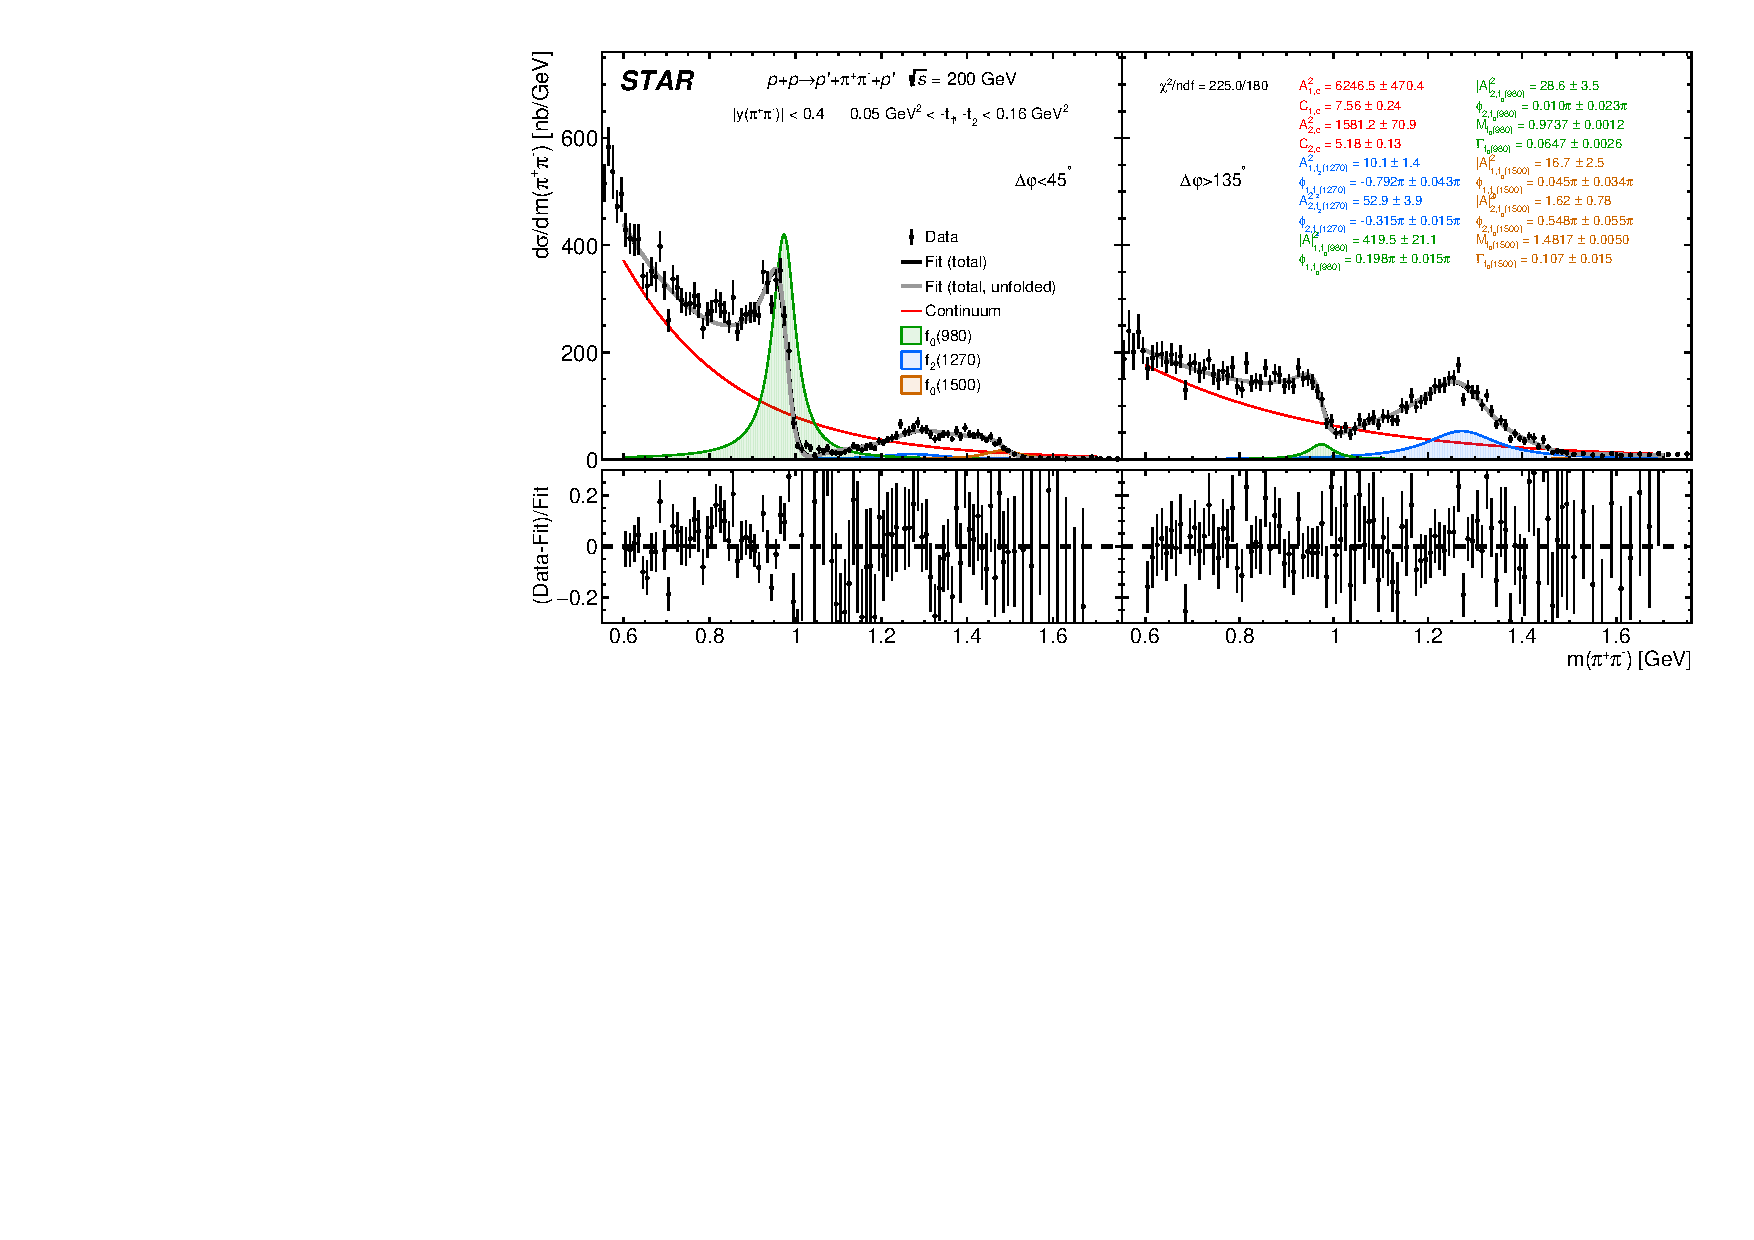
\includegraphics[width=\textwidth,page=1]{graphics/physicsResults/InvMassFit/F0980_BREITWIGNER/Ratio_PiPiInvMass_Fit.pdf}
%
\caption{Extrapolated $d\sigma/dm(\pi^{+}\pi^{-})$ with the fit assuming Breit-Wigner amplitude for $f_{0}(980)$.}
\label{invMassFit_F0980_BREITWIGNER}
\end{figure}

\begin{figure}%[t]
\centering
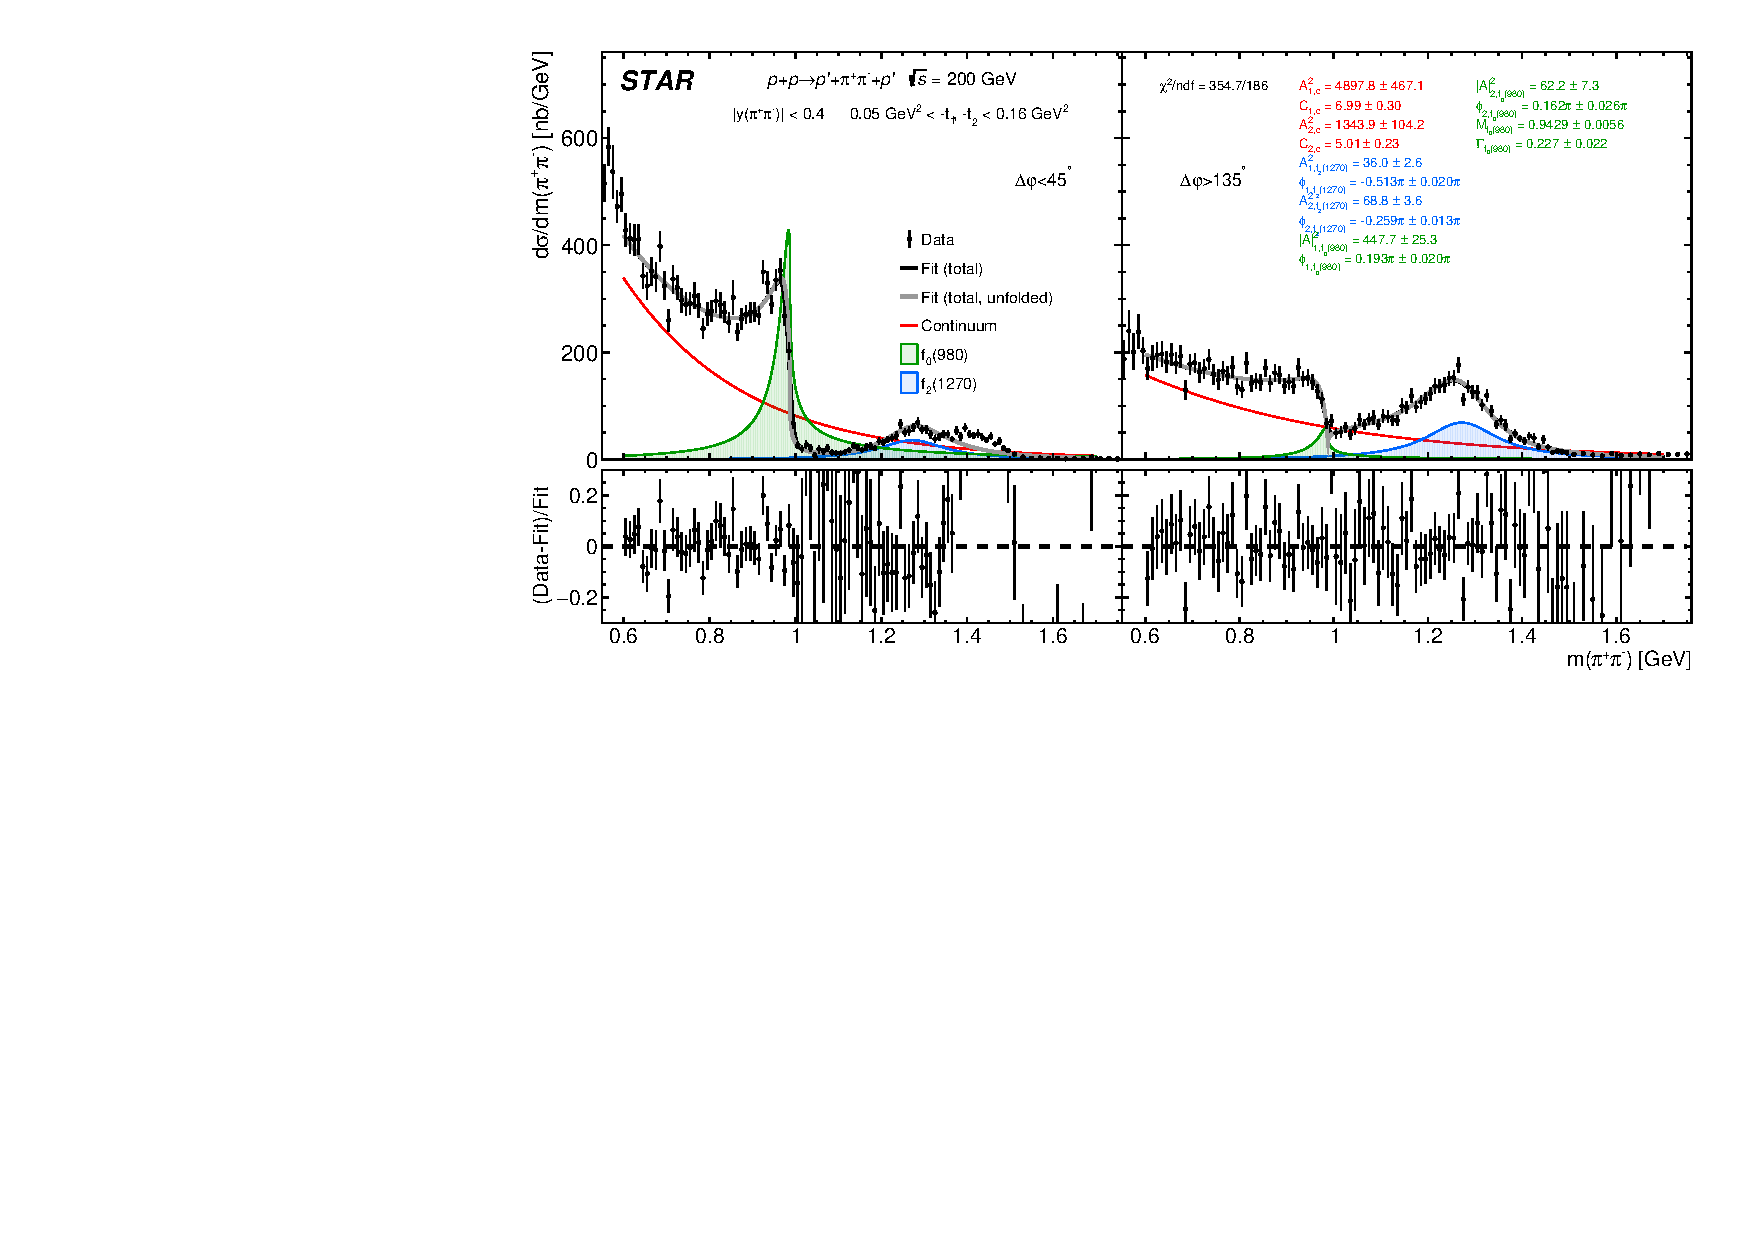
\includegraphics[width=\textwidth,page=1]{graphics/physicsResults/InvMassFit/NO_F01500/Ratio_PiPiInvMass_Fit.pdf}
%
\caption{Extrapolated $d\sigma/dm(\pi^{+}\pi^{-})$ with the fit ignoring $f_{0}(1500)$ component.}
\label{invMassFit_NO_F01500}
\end{figure}

\begin{figure}%[t]
\centering
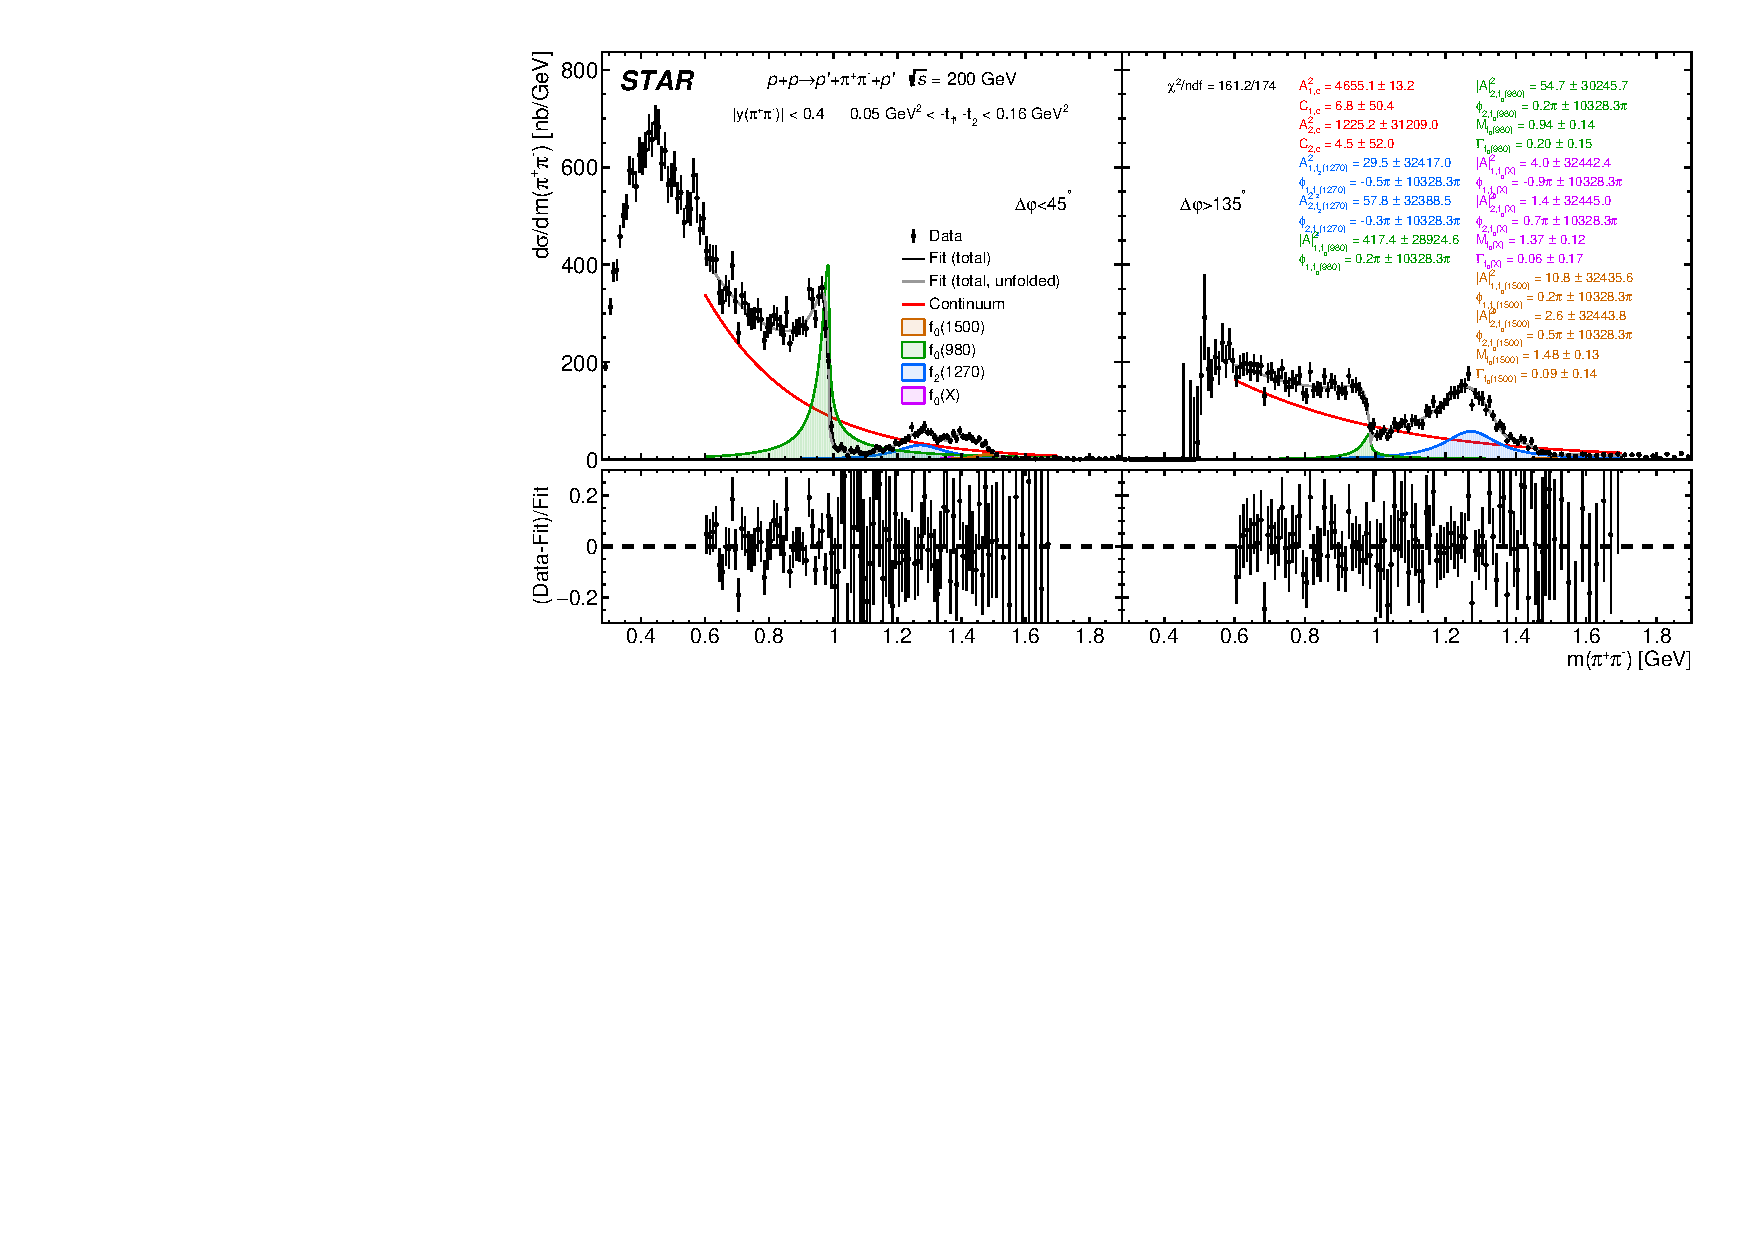
\includegraphics[width=\textwidth,page=1]{graphics/physicsResults/InvMassFit/EXTRA_RESONANCE/Ratio_PiPiInvMass_Fit.pdf}
%
\caption{Extrapolated $d\sigma/dm(\pi^{+}\pi^{-})$ with the fit accounting for an additional $f_{0}(X)$ component.}
\label{invMassFit_EXTRA_RESONANCE}
\end{figure}


% \begin{figure}%[t] 
% \centering
% 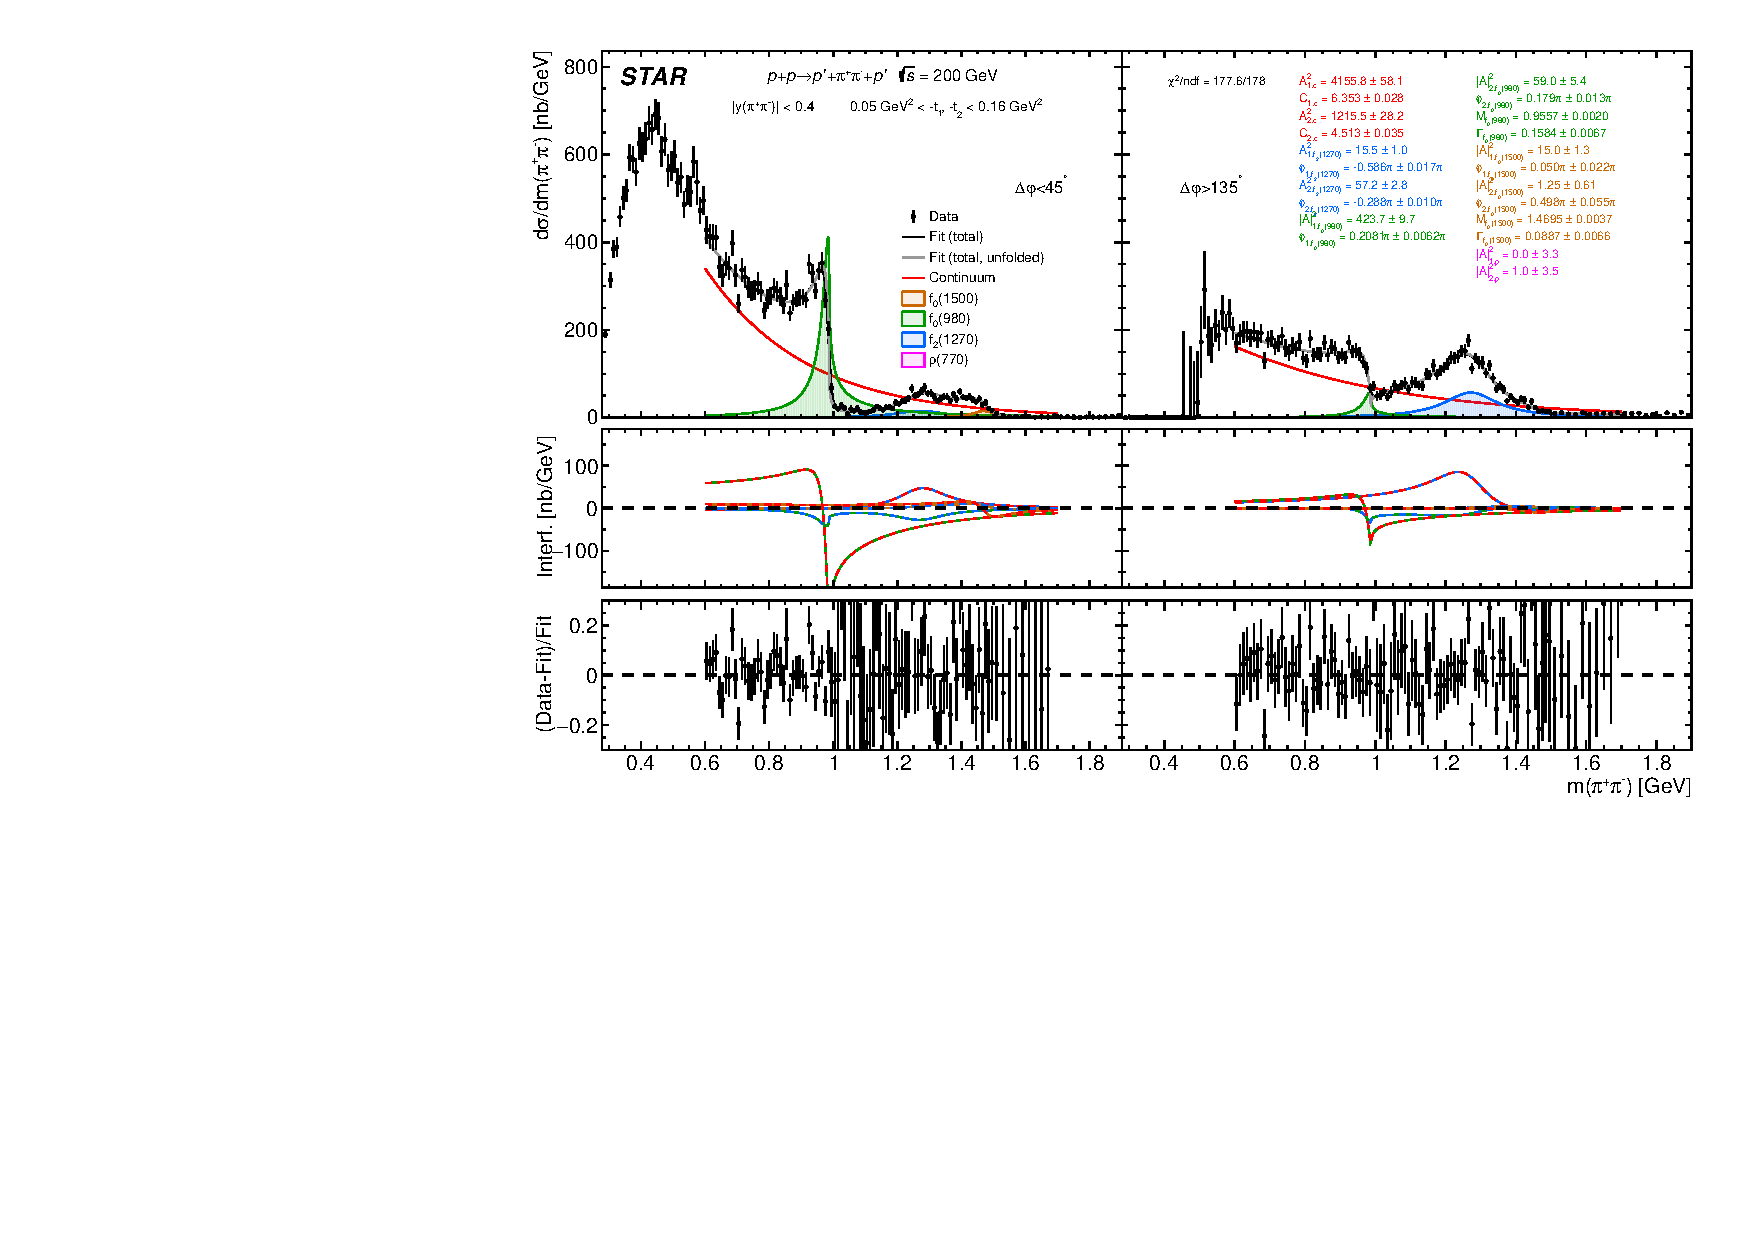
\includegraphics[width=\textwidth,page=1]{graphics/physicsResults/InvMassFit/WITH_RHO/RatioAndInterference_PiPiInvMass_Fit.pdf}
% %
% \caption{Extrapolated $d\sigma/dm(\pi^{+}\pi^{-})$ with the fit accounting for $\rho_{0}(770)$ production.}
% \label{invMassFit_WITH_RHO}
% \end{figure}

%
We have tested a possibility of existence of an additional resonance produced in the mass range $1.2-1.5$ GeV  (Fig.~\ref{invMassFit_EXTRA_RESONANCE}). With $f_0$-like component added to the model from Eq.~\eqref{eq:amplitude} the best fit is achieved for $M_{f_0}=1367 \pm 25 (\text{stat.})$~MeV and $\Gamma_{0,f_0} = 53 \pm 25 (\text{stat.})$~MeV. In that case the $\chi^{2}$/ndf is somewhat improved and equals 161/174 - the dip in $d\sigma/dm(\pi^{+}\pi^{-})$ at 1.32~GeV for $\Delta\varphi<45^{\circ}$ is better described compared to the nominal fit. Other parameters in the fit change slightly and remain compatible with their original values. Noteworthy is increase of the statistical uncertainty of $f_{0}(1500)$ width - $\Gamma_{0,f_0(1500)} = 93 \pm 30 (\text{stat.})$~MeV, which makes it consistent with the PDG average. The fitted content of additional resonance $f_0$ at $\Delta\varphi<45^{\circ}$ is several times lower than extracted yield of $f_{0}(1500)$, while for $\Delta\varphi>135^{\circ}$ it is consistent with 0. The value of mass agrees with that of $f_{0}(1370)$ resonance, however the obtained width is much lower than PDG estimates of about 200-500~MeV.
%

{
\renewcommand{\arraystretch}{1.5}
\begin{table}[]\centering
\begin{tabular}{cc c c}%
~ & \multicolumn{2}{c}{$\bm{\frac{\sigma}{\sigma_{f_{2}(1270)}}}$} & \multirow{2}{*}{$\bm{\frac{\sigma(\Delta\varphi<45^{\circ})}{\sigma(\Delta\varphi>135^{\circ})}}$} \\
~ & $\bm{\Delta\varphi<45^{\circ}}$ & $\bm{\Delta\varphi>135^{\circ}}$ & \\ \hline\hline
$\bm{f_{0}(980)}$ & $8.77 \pm 0.62\,^{+0.58}_{-0.40}\,^{+7.16}_{-0.23}$ & $0.33 \pm 0.03\,^{+0.01}_{-0.01}\,^{+0.13}_{-0.08}$ & $\phantom{1}7.14 \pm 0.66 \,^{+0.18}_{-0.18}\,^{+2.25}_{-0.21}$\\ %\hline
$\bm{f_{2}(1270)}$ & 1 & 1 & $\phantom{1}0.27 \pm 0.02\,^{+0.01}_{-0.01} \,^{+0.02}_{-0.05}$\\ %\hline
$\bm{f_{0}(1500)}$ & $0.49 \pm 0.08\,^{+0.04}_{-0.02}\,^{+0.25}_{-0.05}$ & $0.01 \pm 0.01\,^{+0.00}_{-0.00}\,^{+0.00}_{-0.00}$ & $11.87 \pm 5.76\,^{+0.83}_{-0.67} \,^{+2.09}_{-3.40}$\\ %\hline
\end{tabular}
\caption{Ratios of integrated cross-sections on resonance production. For each ratio a statistical, systematic and model uncertainties are provided, in that order.}\label{tab:resonanceRatio}
\end{table}
}
%
\indent
We also calculated ratios of total cross sections $\sigma_{f_0(980)}/\sigma_{f_2(1270)}$ and $\sigma_{f_0(1500)}/\sigma_{f_2(1270)}$ in two $\Delta \varphi$ regions as well as $\sigma(\Delta \varphi<45^{\circ})/\sigma(\Delta \varphi>135^{\circ})$ for 
all resonances, as listed in Tab.~\ref{tab:resonanceRatio}. In the ratios many of the systematic uncertainties cancelled out.
We observe a significant dependence of the resonance production cross-sections on the azimuthal separation of the forward scattered protons. The two scalar mesons $f_{0}(980)$ and $f_{0}(1500)$ are dominantly produced at $\Delta\varphi<45^{\circ}$, whereas the tensor meson $f_{2}(1270)$ at $\Delta\varphi>135^{\circ}$. This $\Delta\varphi$ dependence is consistent with the observation made by WA102 Collaboration~\cite{WA102}.






\section{Extraction of exponential slope parameter of $d\sigma/dt$}\label{sec:InvMassFit}



Apart from the extrapolation and modelling of the $\pi^{+}\pi^{-}$ invariant mass cross-section we have also applied geometrical corrections to the $d\sigma/dt_{1}dt_{2}$ in the same Lorentz invariant phase-space given by $|y(\pi^+\pi^-)|<0.4$ and $0.05 \leq -t_1 , -t_2 \leq 0.16$ GeV$^2$ and two $\Delta\varphi$ ranges ($\Delta\varphi<45^{\circ}$ and $\Delta\varphi>135^{\circ}$). 
These cross-sections were fitted in two dimensions with the exponent $\propto \exp{\left[\beta t_{1}\right]}\cdot\exp{\left[\beta t_{2}\right]}$ separately in three selected ranges of $m(\pi^{+}\pi^{-})$ (Figs.~\ref{fig:slope_1} and~\ref{fig:slope_2}). Obtained $\beta$ values are provided in Tab.~\ref{tab:slopes}. 
We do not separate modelling uncertainties since they are generally much smaller than experimental uncertainties. This is the consequence of uniform $\varphi$ distribution in all the models and rather weak dependence of the cross-sections within measured $\Delta\varphi$ ranges. Such approximation is well founded and in good agreement with the data.
Variations of the slope $\beta$ with $m(\pi^{+}\pi^{-})$ and $\Delta\varphi$ can give important constrains for model developers.%  For example, it was pointed out~\cite{lebiedowicz_1} that $f_2(1270)$ cross section may show an enhancement when  $t_1\rightarrow 0$, $t_2\rightarrow 0$ for some couplings while for others a suppression is expected which results in respectively larger or smaller value of $\beta$.
%

{
\renewcommand{\arraystretch}{1.5}
\begin{table}[b]\centering
\begin{tabular}{c|| cc}%
~ & $\bm{\Delta\varphi<45^{\circ}}$ & $\bm{\Delta\varphi>135^{\circ}}$\\ \hline\hline
$\bm{0.6~\text{\bf{GeV}} < m <1~\text{\bf{GeV}}}$ & $8.65 \pm 0.28 \,^{+0.91}_{-0.69}$ & $13.95 \pm 0.47\,^{+0.57}_{-0.95}$\\ %\hline
$\bm{1~\text{\bf{GeV}} < m < 1.5~\text{\bf{GeV}}}$ & $9.78 \pm 0.65 \,^{+0.70}_{-0.74}$ & $\phantom{1}4.34 \pm 0.40\,^{+0.73}_{-0.77}$\\ %\hline
$\bm{m>1.5~\text{\bf{GeV}}}$ & $8.00 \pm 1.16\,^{+0.75}_{-0.79}$ & $\phantom{1}4.67 \pm 0.97\,^{+0.78}_{-0.84}$\\ %\hline
\end{tabular}
\caption{Slope $\beta$ (in GeV$^{-2}$) of the $-t$ distribution in three ranges of $m(\pi^{+}\pi^{-})$ and two two ranges of $\Delta\varphi$. For each number a statistical and systematic uncertainties are provided, in that order.}\label{tab:slopes}
\end{table}
}


\begin{figure}%[t]
\centering
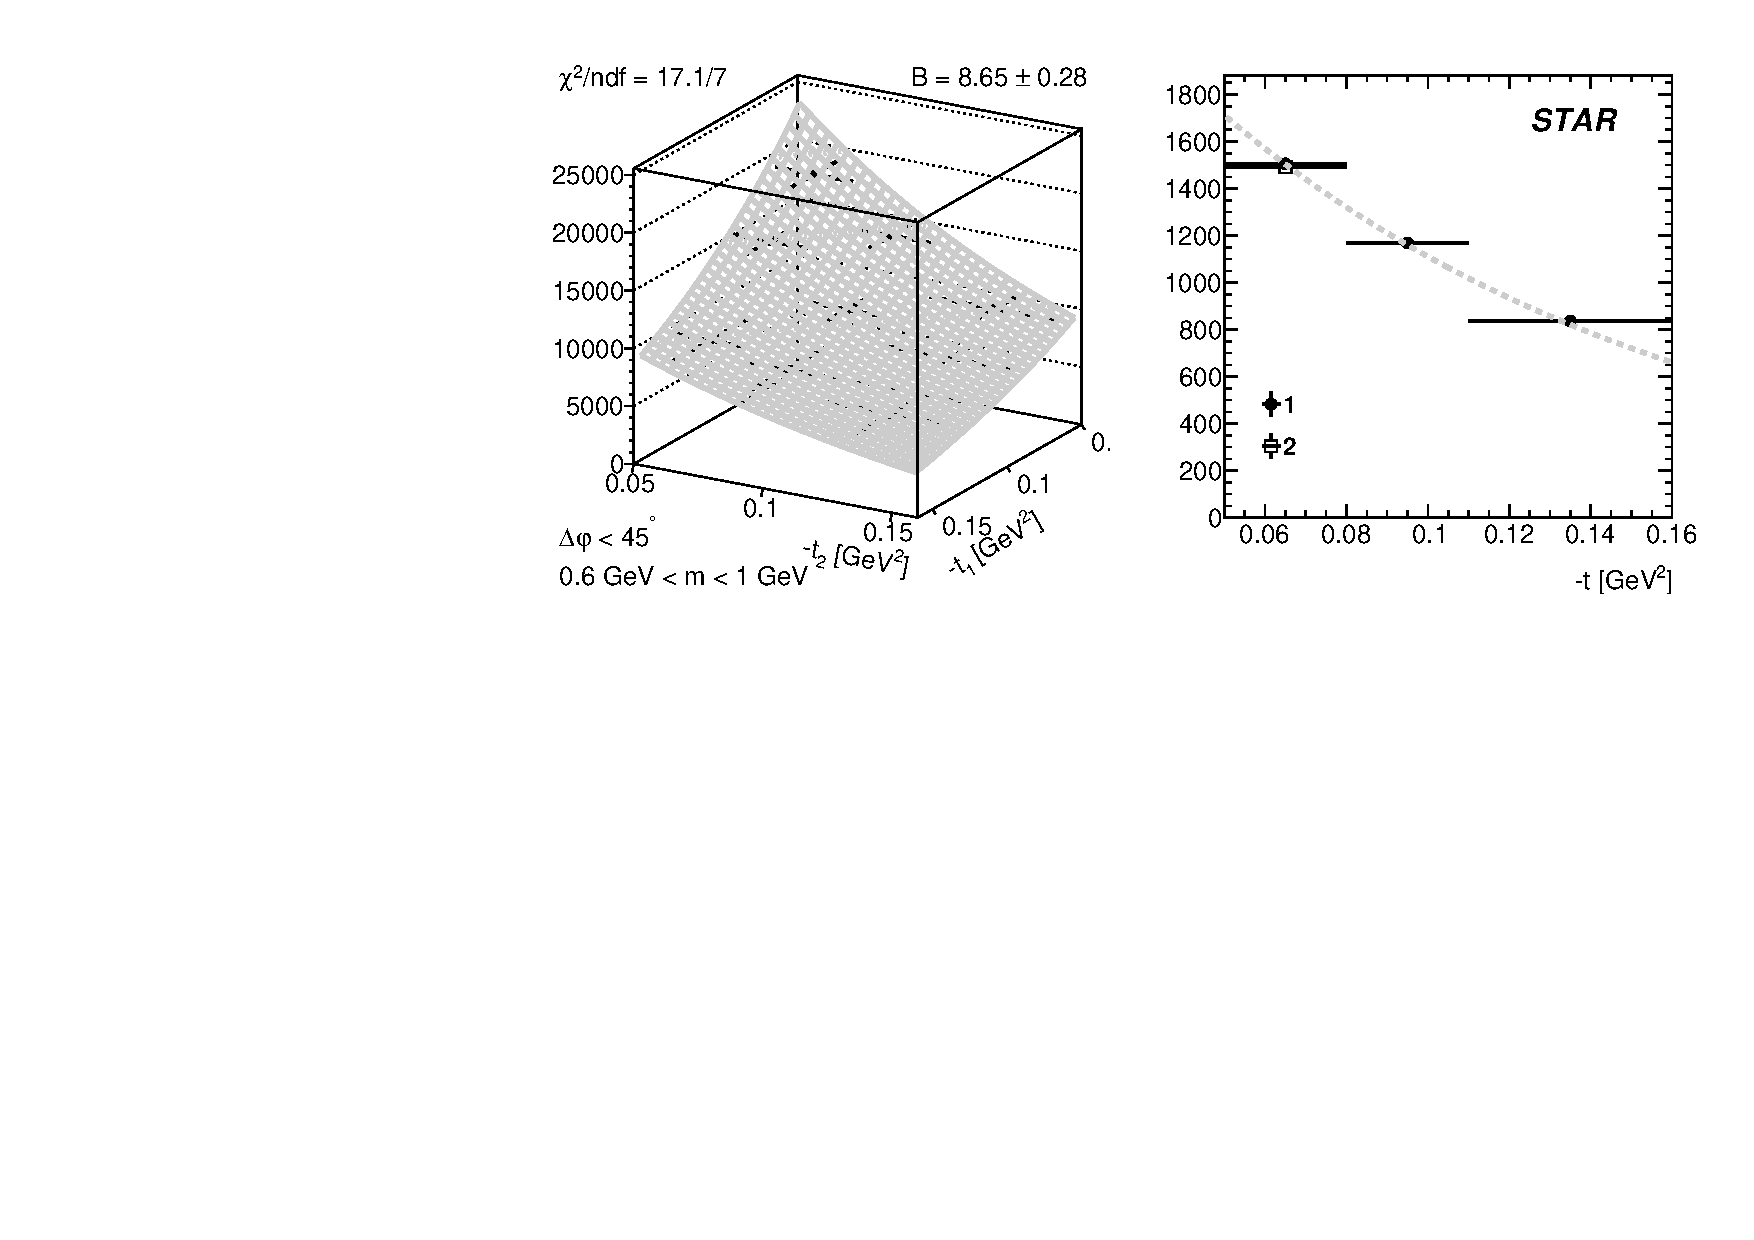
\includegraphics[width=0.9\textwidth,page=1]{graphics/physicsResults/SlopeExtraction.pdf}\\[7pt]
\includegraphics[width=0.9\textwidth,page=2]{graphics/physicsResults/SlopeExtraction.pdf}\\[7pt]
\includegraphics[width=0.9\textwidth,page=3]{graphics/physicsResults/SlopeExtraction.pdf}
%
\caption{Extrapolated $d^{2}\sigma/dt_{1}dt_{2}$ for $\Delta\varphi<45^{\circ}$ with the exponential fit (left) and projections on the $t_{1}$ and $t_{2}$ axes (right) in three mass ranges provided in the plots.}
\label{fig:slope_1}
\end{figure}


\begin{figure}%[t]
\centering
\includegraphics[width=0.9\textwidth,page=4]{graphics/physicsResults/SlopeExtraction.pdf}\\[7pt]
\includegraphics[width=0.9\textwidth,page=5]{graphics/physicsResults/SlopeExtraction.pdf}\\[7pt]
\includegraphics[width=0.9\textwidth,page=6]{graphics/physicsResults/SlopeExtraction.pdf}
%
\caption{Extrapolated $d^{2}\sigma/dt_{1}dt_{2}$ for $\Delta\varphi>135^{\circ}$ with the exponential fit (left) and projections on the $t_{1}$ and $t_{2}$ axes (right) in three mass ranges provided in the plots.}
\label{fig:slope_2}
\end{figure}
